% Options for packages loaded elsewhere
\PassOptionsToPackage{unicode}{hyperref}
\PassOptionsToPackage{hyphens}{url}
%
\documentclass[
]{article}
\usepackage{amsmath,amssymb}
\usepackage{iftex}
\ifPDFTeX
  \usepackage[T1]{fontenc}
  \usepackage[utf8]{inputenc}
  \usepackage{textcomp} % provide euro and other symbols
\else % if luatex or xetex
  \usepackage{unicode-math} % this also loads fontspec
  \defaultfontfeatures{Scale=MatchLowercase}
  \defaultfontfeatures[\rmfamily]{Ligatures=TeX,Scale=1}
\fi
\usepackage{lmodern}
\ifPDFTeX\else
  % xetex/luatex font selection
\fi
% Use upquote if available, for straight quotes in verbatim environments
\IfFileExists{upquote.sty}{\usepackage{upquote}}{}
\IfFileExists{microtype.sty}{% use microtype if available
  \usepackage[]{microtype}
  \UseMicrotypeSet[protrusion]{basicmath} % disable protrusion for tt fonts
}{}
\makeatletter
\@ifundefined{KOMAClassName}{% if non-KOMA class
  \IfFileExists{parskip.sty}{%
    \usepackage{parskip}
  }{% else
    \setlength{\parindent}{0pt}
    \setlength{\parskip}{6pt plus 2pt minus 1pt}}
}{% if KOMA class
  \KOMAoptions{parskip=half}}
\makeatother
\usepackage{xcolor}
\usepackage{longtable,booktabs,array}
\usepackage{calc} % for calculating minipage widths
% Correct order of tables after \paragraph or \subparagraph
\usepackage{etoolbox}
\makeatletter
\patchcmd\longtable{\par}{\if@noskipsec\mbox{}\fi\par}{}{}
\makeatother
% Allow footnotes in longtable head/foot
\IfFileExists{footnotehyper.sty}{\usepackage{footnotehyper}}{\usepackage{footnote}}
\makesavenoteenv{longtable}
\usepackage{graphicx}
\makeatletter
\def\maxwidth{\ifdim\Gin@nat@width>\linewidth\linewidth\else\Gin@nat@width\fi}
\def\maxheight{\ifdim\Gin@nat@height>\textheight\textheight\else\Gin@nat@height\fi}
\makeatother
% Scale images if necessary, so that they will not overflow the page
% margins by default, and it is still possible to overwrite the defaults
% using explicit options in \includegraphics[width, height, ...]{}
\setkeys{Gin}{width=\maxwidth,height=\maxheight,keepaspectratio}
% Set default figure placement to htbp
\makeatletter
\def\fps@figure{htbp}
\makeatother
\ifLuaTeX
  \usepackage{luacolor}
  \usepackage[soul]{lua-ul}
\else
  \usepackage{soul}
\fi
\setlength{\emergencystretch}{3em} % prevent overfull lines
\providecommand{\tightlist}{%
  \setlength{\itemsep}{0pt}\setlength{\parskip}{0pt}}
\setcounter{secnumdepth}{-\maxdimen} % remove section numbering
\ifLuaTeX
  \usepackage{selnolig}  % disable illegal ligatures
\fi
\IfFileExists{bookmark.sty}{\usepackage{bookmark}}{\usepackage{hyperref}}
\IfFileExists{xurl.sty}{\usepackage{xurl}}{} % add URL line breaks if available
\urlstyle{same}






\usepackage[a4paper,margin=1in]{geometry}
\usepackage{xcolor}
\usepackage{pagecolor}
\usepackage{titlesec}
\usepackage{soul}
\usepackage[export]{adjustbox}

\usepackage{fancyhdr}
\usepackage{lastpage}
\pagestyle{fancy}
\fancyhf{}
\lhead{Group 11 Wicked Reality}
\rfoot{Page \thepage\ of \pageref{LastPage}}
\renewcommand{\headrulewidth}{0.4pt}
\renewcommand{\footrulewidth}{0.4pt}

\definecolor{darkbg}{HTML}{1E1E1E}
\definecolor{lighttext}{HTML}{D4D4D4}
\definecolor{titleorange}{HTML}{FF8C00}
\definecolor{subtitleblue}{HTML}{569CD6}

\pagecolor{darkbg}
\color{lighttext}

% Center all images globally
\makeatletter
\let\old@includegraphics\includegraphics
\renewcommand{\includegraphics}[2][]{\begin{center}\old@includegraphics[#1]{#2}\end{center}}
\makeatother

% Heading colors
\titleformat{\section}{\color{titleorange}\normalfont\Large\bfseries}{\thesection}{1em}{}
\titleformat{\subsection}{\color{subtitleblue}\normalfont\large\bfseries}{\thesubsection}{1em}{}
\titleformat{\subsubsection}{\color{lighttext}\normalfont\normalsize\bfseries}{\thesubsubsection}{1em}{}

\lhead{\color{lighttext}Group 11 Wicked Reality}
\rfoot{\color{lighttext}Page \thepage\ of \pageref{LastPage}}

\hypersetup{colorlinks=true, linkcolor=cyan, urlcolor=cyan}
\begin{document}

\begin{titlepage}
    \centering
    \thispagestyle{empty}
    \vspace*{2cm}
    
    {\Large\bfseries \color{lighttext} Group 11 Wicked Reality \par}
    \vspace{2cm}
    
    {\Huge\bfseries \color{titleorange} Requirements Documentation \par}
    \vspace{0.5cm}
    {\LARGE \color{lighttext} Wicked Reality (Group 9) \par}
    
    \vspace{2cm}
    {\Large \color{lighttext} Development Team: Group 11 \par}
    \vspace{1cm}
    
    {\large \color{lighttext} \textbf{Group Members}: \par}
    {\large \color{lighttext} Arika Khor, Cambren Williams, Ephraim Wong, \par}
    {\large \color{lighttext} Ethan Gulley, Jax Breedlove Donlon, Thuan Nguyen \par}
    
    \vfill
    {\large \color{lighttext} May 3, 2026 \par}
\end{titlepage}
\newpage
\setcounter{page}{1}

Revision History

\begin{longtable}[]{@{}
  >{\raggedright\arraybackslash}p{(\columnwidth - 6\tabcolsep) * \real{0.4615}}
  >{\raggedright\arraybackslash}p{(\columnwidth - 6\tabcolsep) * \real{0.1939}}
  >{\raggedright\arraybackslash}p{(\columnwidth - 6\tabcolsep) * \real{0.2324}}
  >{\raggedright\arraybackslash}p{(\columnwidth - 6\tabcolsep) * \real{0.1122}}@{}}
\toprule\noalign{}
\begin{minipage}[b]{\linewidth}\raggedright
Name
\end{minipage} & \begin{minipage}[b]{\linewidth}\raggedright
Date
\end{minipage} & \begin{minipage}[b]{\linewidth}\raggedright
Reason for Changes
\end{minipage} & \begin{minipage}[b]{\linewidth}\raggedright
Version
\end{minipage} \\
\midrule\noalign{}
\endhead
\bottomrule\noalign{}
\endlastfoot
First Draft of Requirements Documentation & Feb/22/2026 & Initial Draft
& 1 \\
Second Draft of Requirements Documentation & April/05/2026 & Secondary
Addition to Additional Requirements & 2 \\
Third Draft of Requirements Documentation & May/01/2026 & Third Addition
to Additional Requirements & 3 \\
\end{longtable}

\tableofcontents
\newpage
\phantomsection \phantomsection\section{1. Overview}\label{overview}

Wicked Realty is commissioning the development of a residential real
estate Fair Value Estimate (FVE) engine to modernize and automate its
property valuation process. Currently, the firm relies on manual
calculations performed by realtors to determine market values, a process
that is both time-consuming and error-prone. This new FVE engine will
replace subjective ``gut feel'' valuations with standardized, defensible
reports through a Python-based command line interface (CLI). By
integrating features such as Geospatial Location Weighting and
Adjustment Logic for specific home features, the FVE engine aims to
provide consistent and rapid Comparative Market Analysis (CMA) reports.
Ultimately, the FVE engine will serve as a single source of truth for
Wicked Realty and support high-volume market valuation analysis to allow
realtors and agents to focus on customer relations.

\phantomsection \phantomsection\section{2. Business Requirements}\label{business-requirements}

a. Background

Wicked Realty lacks an automated system for generating FVE of
residential properties in Norman, forcing realtors to perform all CMA
calculations manually. This manual process relies on metrics such as the
number of bedrooms, bathrooms, square footage, and a number of other
relevant factors. However, since these CMAs are performed by
individuals, the FVEs generated are highly susceptible to ``gut feel''
biases and human error. Wicked Reality wants an algorithm to rapidly
compute the FVE of properties from a CMA perspective more efficiently
and effectively serve their customers by providing a plethora of data
driven FVE.

b. Business Opportunities

Wicked Realty's current bottleneck in getting an estimate for potential
home buyers is doing the manual calculations on what the FVE of a home
is. The FVE engine will algorithmically compute consistent FVEs, heavily
reducing human workload and dramatically speeding up the CMA process.
This also reduces possible errors caused by realtors overlooking or
miscalculating figures. Overall, this product will increase
organizational efficiency, reduce errors, and provide a more consistent
output for the realtors and Wicked Realty's customers.

c. Business Objectives

\begin{itemize}
\item
  The average time to calculate the FVE on a residential property should
  be reduced from 1 hour to under 1 minute immediately after
  implementing the system.
\item
  The average time to calculate multiple FVEs, to a maximum of 100,
  should be reduced from multiple business days to under 5 minutes
  immediately after implementation of the system.
\item
  The volume of property appraisals handled by Wicked Realty per week
  should increase by 40\% over the following month after implementing
  the system.
\end{itemize}

d. Success Metrics

\begin{itemize}
\item
  ROI is calculated as
\end{itemize}

\begin{quote}
\[ROI\, = \,\frac{WagesSaved\, - FVECost}{FVECost}\]
\end{quote}

where the wages saved are

\begin{quote}
\[WagesSaved\, = \, TimeSaved \cdot EmployeeHourly \cdot NumEmployees\ \]
\end{quote}

and FVE Cost is the cost of developing and maintaining the FVE engine,
which will be close to zero. Ideally, a high ROI of over 300\% should be
achieved.

\begin{itemize}
\item
  Accuracy delta is measured as the average accuracy of the FVE minus
  the average accuracy of the realtors, where accuracy is measured as
\end{itemize}

\begin{quote}
\[\text{Accuracy} = 1 - \left| \frac{Estimate - Actual}{Actual} \right|\]
\end{quote}

The accuracy delta should be at least 2\%.

\begin{itemize}
\item
  DOM is calculated as
\end{itemize}

\begin{quote}
\[\text{Average}\text{ }\text{DOM} = \frac{\sum_{\text{ }}^{\text{ }}\text{Days}\text{ }\text{on}\text{ }\text{Market}}{n}\]
\end{quote}

where n is the number of properties. As the algorithm will run faster
and be more accurate than realtors, the average DOM should drop by at
least 10\%.

e. Product Vision Statement

For Wicked Realty realtors and agents who need to rapidly generate
accurate and consistent FVEs for residential properties without relying
on slow, error-prone manual calculations, the FVE engine is a
centralized, Python-based algorithmic tool that will provide standard
Python-based, feasible, and transparent valuations by automating CMA
through geospatial weighting and adjustment logic. Unlike Wicked
Realty's current manual processes that consume significant man-hours and
rely on subjective ``gut feel'', the FVE engine eliminates the human
element from core computations, maximizing operational efficiency by
reducing CMA computation time from one hour to under 5 minutes and
allowing realtors to focus on customer relations and sales.

\phantomsection \phantomsection\section{3. Scope and Limitations}\label{scope-and-limitations}

a. Major Features

\begin{itemize}
\item
  FVE calculation for a single property
\item
  FVE calculation for a batch of properties of up to 100 properties
\item
  Comprehensive CMA Input Engine that allows for custom inputs
\item
  Geospatial Location Weighting for neighborhood specific premiums
\item
  Standardized Adjustment Logic that allows for custom weights
\end{itemize}

b. Project Scope

The scope of this project involves the development of an FVE engine to
provide a standardized, defensible, and transparent framework for
property valuation, moving away from subjective ``gut feel'' estimates.
By automating the CMA process, the tool aims to eliminate the human
element from core computation processes, thereby mitigating calculation
errors and implementing a consistent and scalable computation operation
across the entire agency. This tool strategically aligns with Wicked
Realty's long-term goals of maximizing operational efficiency; by
offloading data-heavy analytics to computers, realtors are freed to
focus on customer relations and sales. This project directly supports
the corporate goal of digital transformation, positioning Wicked Realty
as a data-driven leader in local markets. The software will serve as a
single source of truth for all residential listings, enabling
inter-agent and inter-departmental collaboration while lowering the
barrier to entry for realtors to be effective in this field of work.

c. Limitations and Exclusions

To maintain project focus and ensure timely delivery, certain
functionalities have been explicitly excluded from the current scope.
Firstly, the FVE engine will provide a snapshot valuation only and will
not include predictive forecasting or market trend modeling; the tool is
designed to deliver a property's current FVE rather than future
appreciation. Secondly, the system will be developed to FVE generation
of residential property listings. The algorithmic logic will be
calibrated for housing metrics and cannot accurately support commercial
real estate, which is affected by starkly different factors, making it a
uniquely different product.

Thirdly, automated data scraping is excluded from this release. While
integration with large third-party platforms such as Zillow, Homes.com,
Realtor.com, and other property listing marketplace platforms is a
potential future iteration, the current version will require all input
parameters to be handled by the firm's staff. The development will
provide an initial dataset alongside the pre-beta release to show
working proof of concept.

These exclusions are intentional to prioritize the core FVE engine
accuracy and tailor the system's overall ease of use for Wicked Realty's
staff. By defining these boundaries, the team can ensure timely delivery
of a stable, reliable tool that meets Wicked Realty's immediate internal
requirements whilst balancing the cost, maintenance, and integration
complexities of external dependencies.

\phantomsection \phantomsection\section{4. Context Description}\label{context-description}

a. User Classes and Characteristics

The product has 3 main user classes to be implemented. The primary user
class is the realtors. Realtors should be the main users of the product,
possibly using it every day. Realtors are expected to have high
knowledge of the parameters and should be able to identify values for
each parameter. However, there is no expectation that the realtors
should have any technical knowledge. Clear labels must be included on
every interface, using only terminology that realtors should be
comfortable with. Important actions should be highlighted to grab
attention. New users should be able to create an output within 5
minutes. Error messages should describe the problem and what is
necessary for the user to fix it.

The administrative managers (managers) are a secondary user class. They
are expected to have no technical knowledge. Managers' primary use case
is for reading high-level reports and managing the realtors. Managers
are responsible for managing realtors\textquotesingle{} access to the
product. This includes providing and removing access to the realtors.

I.T. administrators and software developers are a secondary user class
responsible for maintaining the product post launch. They should be
responsible for bug fixes and updating the algorithm as the market
shifts. They are expected to have some technical expertise. The UI for
the IT/Dev user class should have clear labels and descriptive error
messages.

b. Operating Environment

The software will operate within Wicked Realty\textquotesingle s
internal computer network. It will be a simple, text-based program
(known as a command line interface) built using Python. Employees just
need a standard computer that can open text-based programs and basic
charts. The program must work smoothly alongside spreadsheet software
like Microsoft Excel and Google Sheets, so users can easily load and
save their housing data. It might also need to connect to the
company\textquotesingle s secure databases to store this information
safely.

c. Design and Implementation Constraints

The development of the FVE engine is governed by several strict
technical and operational constraints designed to ensure immediate
usability and long-term sustainability. The primary interface
deliverable must be a CLI built using Python. To maintain data security
and operational independence, the system will be built to support
locally hosted housing data and will be restricted from using external
APIs, although this is possible for future iterations. The engine must
be maintainable, allowing non-technical managers, realtors, and agents
to adjust factor weights, such as neighborhood premiums or feature
modifiers, through external configuration rather than requiring code
changes, ensuring the FVE engine remains adaptable and current to market
shifts.

d. Assumptions and Dependencies

This project operates under a few assumptions based on data, users, and
maintenance. First, it is assumed that information about housing data
will be up to date, sufficient, accurate, and stored in a CSV format.
Furthermore, we assume that the housing data will be complete,
consistent, and represent the area where the house is located
accurately. It is assumed that end users will have access to computers
capable of running console applications and basic data visualization
tools. As for post development lifecycle, the project assumes that
Wicked Realty will allocate necessary personnel and resources to
maintain and upkeep the system and data updates. Finally, the
development of the system is going to be heavily dependent on using the
Python programming language, and scikit learn machine learning library
to build the predictive model, alongside the strict dependency that all
historical data must be queried from a CSV file rather than from an
external API.

e. Glossary of Terms

Fair Value Estimate (FVE)

Fair Value Estimate refers to a standardized, market adjusted valuation
of real estate listings after variables such as housing conditions,
property features, and other relevant variables are taken into account.

Comparative Market Analysis (CMA)

A method used by real estate professionals to estimate the value of a
property by evaluating similar listings within an area to determine a
fair and competitive market price.

Geospatial Location Weighting

A mathematical adjustment applied to the valuation algorithm that
accounts for the geographical desirability of specific neighborhoods and
zones.

Comma separated List (CSV)

A file format for storing data in a tabular format where values are
separated by commas and organized into rows and columns

Command line (CLI)

A user interface used to run programs

Return of Investment (ROI)

A performance measure used to evaluate the efficiency of an investment.
This is calculated by using the (annual return / total investment) x
100. In the context of real estate, we are aiming for 10\% or higher to
be classified as `strong'

Application programming interface (API)

A set of rules and protocols that allow different software applications
to communicate and exchange data with each other using functions such as
"GET" and "POST."

Accuracy Delta

The numerical difference between the fair value price predicted by the
algorithm and the actual final sale price of the property; used as a
primary metric to evaluate the model\textquotesingle s performance.

Days on market (DOM)

total number of days from the date a property is first listed in the
system to the day of its sale if applicable

User interface (UI)

Regression Model

A type of machine learning algorithm used to predict a continuous
numerical value

IT/Dev

personnel responsible for the technical deployment, hosting environment,
and long-term maintenance

f. References

Real Estate Price Listing Websites

\begin{itemize}
\item
  Source: Zillow and Apartments.com.
\end{itemize}

\begin{itemize}
\item
  Location: zillow.com and apartments.com.
\end{itemize}

\begin{itemize}
\item
  Purpose: External web addresses referenced for researching the price,
  square footage, and attributes of homes in the assumed area.
\end{itemize}

Wicked Realty Housing Price Predictions RPF

\begin{itemize}
\item
  Authors: Wicked Realty Project Team 9 (Steven Tran, Sean Ropp, Trevor
  Bean, Caleb Furley, Alex Requena, Abhinav Pillai).
\item
  Version: 1.0
\item
  Date: January 28, 2026.
\item
  Purpose: The primary source document establishing the
  project\textquotesingle s background, objectives, and constraints.
\end{itemize}

\phantomsection \phantomsection\section{5. System Features}\label{system-features}

\ul{System Feature 1: Docker Image}

Priority: MEDIUM

Description: The Docker Image feature packages the FVE engine along with
all necessary dependencies and environment configuration into a single,
standardized container. This ensures that the application runs
identically across different workstations and operating systems --
mitigating the need for onerous installations and configuration --
simplifying deployment and maintenance.

Functional Requirements: These are the software capabilities that must
be present in order for the user to carry out the services provided by
the feature, or to execute related use case(s).

\begin{enumerate}
\def\labelenumi{\Roman{enumi})}
\item
  DOC-REQ-1: Containerized Runtime Environment

  \begin{enumerate}
  \def\labelenumii{\alph{enumii}.}
  \item
    Responding to Anticipated Error Conditions

    \begin{enumerate}
    \def\labelenumiii{\roman{enumiii}.}
    \item
      Missing Docker Daemon
    \end{enumerate}
  \end{enumerate}
\end{enumerate}

\begin{quote}
If the user attempts to run the initialization script before the Docker
engine is installed or running on the host machine, the setup script
shall gracefully exit and echo ``Docker not found'' error.
\end{quote}

\begin{enumerate}
\def\labelenumi{\roman{enumi}.}
\setcounter{enumi}{1}
\item
  Insufficient Resources
\end{enumerate}

\begin{quote}
If the host machine does not meet the minimum memory allocations
required by the container, the container shall gracefully fail on
startup and log an ``Insufficient Memory Allocation'' error.
\end{quote}

\begin{enumerate}
\def\labelenumi{\alph{enumi}.}
\setcounter{enumi}{1}
\item
  Backward Traceability

  \begin{enumerate}
  \def\labelenumii{\roman{enumii}.}
  \item
    Source
  \end{enumerate}
\end{enumerate}

\begin{itemize}
\item
  Client Meeting -- 02/09/2026

  \begin{enumerate}
  \def\labelenumi{\roman{enumi}.}
  \item
    Rational
  \end{enumerate}
\end{itemize}

\begin{quote}
After discussion with the client about operating system capability
constraints, the development team determined that an isolated container
prevents Environmental Inconsistency errors. Running the CLI application
also allows for easy version control without managing complex
environments across the firm.
\end{quote}

\begin{enumerate}
\def\labelenumi{\alph{enumi}.}
\item
  Forward Traceability
\end{enumerate}

\begin{quote}
User Acceptance Testing: After deploying the image onto a clean test
host computer, if the CLI application runs successfully, this
requirement is met and verified.
\end{quote}

\begin{enumerate}
\def\labelenumi{\Roman{enumi})}
\setcounter{enumi}{1}
\item
  DOC-REQ-2: Local Data Volume Mounting

  \begin{enumerate}
  \def\labelenumii{\alph{enumii}.}
  \item
    Responding to Anticipated Error Conditions

    \begin{enumerate}
    \def\labelenumiii{\roman{enumiii}.}
    \item
      Volume Mount Permission Denied
    \end{enumerate}
  \end{enumerate}
\end{enumerate}

\begin{quote}
If the container attempts to access a protected local directory or lacks
read/write permission for target folders, the CLI shall echo a storage
access error and exit execution with exit code in accordance with
CLI-REQ-1.
\end{quote}

\begin{enumerate}
\def\labelenumi{\alph{enumi}.}
\setcounter{enumi}{1}
\item
  Backward Traceability

  \begin{enumerate}
  \def\labelenumii{\roman{enumii}.}
  \item
    Source
  \end{enumerate}
\end{enumerate}

\begin{itemize}
\item
  RFP Section 6.0
\item
  RFP Section 7.0

  \begin{enumerate}
  \def\labelenumi{\roman{enumi}.}
  \item
    Rationale
  \end{enumerate}
\end{itemize}

\begin{quote}
The system will use local CSV data for this current iteration of
application since cloud integrations are complex and will delay the
development cycle of the application. However, it is possible to stub
out potential external API and cloud integrations for future
development.
\end{quote}

\begin{enumerate}
\def\labelenumi{\alph{enumi}.}
\item
  Forward Traceability
\end{enumerate}

\begin{quote}
Integration Testing can verify that CSV files placed in predetermined
local host directories can be successfully ingested by the containerized
CLI application, and that resulting reports can be saved to
predetermined local host directories.
\end{quote}

Use Cases:

\begin{itemize}
\item
  DOC-REQ-1: The system shall successfully instantiate the Docker
  container and present the application CLI prompt to the user in no
  more than THIRTY (30) seconds of executing the run command.
\item
  DOC-REQ-2: Upon composing the Docker container, the system shall
  initialize the container and establish a read/write connection to the
  configured local folders within TEN (10) seconds.
\end{itemize}

Use Case Flow:

\begin{enumerate}
\def\labelenumi{\arabic{enumi}.}
\item
  User downloads the WIcked Realty FVE engine Docker image to their
  local workstation.
\item
  User runs the initialization command mapped to their local CSV storage
  directory, triggering DOC-REQ-2.
\item
  System triggers DOC-REQ-1 which unpacks necessary environments and
  dependencies without touching the host OS registry.
\item
  System presents the active CLI application to the user.
\end{enumerate}

User Stories:

User 1

\begin{quote}
Narrative:
\end{quote}

\begin{itemize}
\item
  As an I.T. Administrator,
\item
  I want to deploy the CLI application as a pre-packaged Docker image,
\item
  so that I will not have to manually install all environments,
  versions, and dependencies on every single workstation.
\end{itemize}

\begin{quote}
Acceptance:
\end{quote}

\begin{itemize}
\item
  Given a new workstation with Docker engine installed,
\item
  When I pull Wicked Realty FVE engine Docker image and execute the
  docker run command,
\item
  Then the CLI application will be fully operational and ready for use
  without any further setup.
\end{itemize}

User 2

\begin{quote}
Narrative:
\end{quote}

\begin{itemize}
\item
  As a Real Estate Agent,
\item
  I want to run the application easily on my local computer with my
  local files,
\item
  so that I will not have to go through extensive setup before using the
  application to generate reports.
\end{itemize}

\begin{quote}
Acceptance:
\end{quote}

\begin{itemize}
\item
  Given CSV files in my local host folders,
\item
  When I launch the application and run designated commands,
\item
  Then the application can read my local CSVs and save reports onto my
  local folders.
\end{itemize}

\ul{System Feature 2: Command Line Interface Application}

Priority: HIGH

Description: Provides a lightweight, text-based interface within a
terminal for users.

Functional Requirements

\begin{enumerate}
\def\labelenumi{\Roman{enumi})}
\item
  CLI-REQ-1: Command Execution \& Parsing

  \begin{enumerate}
  \def\labelenumii{\alph{enumii}.}
  \item
    Responding to Anticipated Error Conditions

    \begin{enumerate}
    \def\labelenumiii{\roman{enumiii}.}
    \item
      \begin{quote}
      Missing Dependencies
      \end{quote}
    \end{enumerate}
  \end{enumerate}
\end{enumerate}

\begin{quote}
If commands require external files that are not found, the CLI shall
provide the specific path, file name, and file extension of where and
what was expected.
\end{quote}

\begin{enumerate}
\def\labelenumi{\roman{enumi}.}
\setcounter{enumi}{1}
\item
  Program Execution Error
\end{enumerate}

\begin{quote}
If a program exits with any code other than a success code (CODE:0), the
CLI shall:
\end{quote}

\begin{itemize}
\item
  \textbf{Terminate Execution}: Immediately halt the current process to
  prevent cascading errors and further data corruption.
\item
  \textbf{Return Standard Error}: Output a concise, human-readable error
  message to `stderr` which highlights exactly which step failed.
\item
  \textbf{Log the Exit Code}: Echo the exit code with brief description
  to assist troubleshooting. I.e `Exit Code 124: Command Time Out`.

  \begin{enumerate}
  \def\labelenumi{\alph{enumi}.}
  \item
    Backward Traceability (rationale for the requirements and the source
    -- RFP and which section in it, client meeting and which notes from
    that meeting, etc.)
  \item
    Forward Traceability

    \begin{enumerate}
    \def\labelenumii{\roman{enumii}.}
    \item
      \textbf{Verification}
    \end{enumerate}
  \end{enumerate}
\end{itemize}

\begin{enumerate}
\def\labelenumi{\arabic{enumi}.}
\item
  User Acceptance Testing (UAT) via terminal execution using Blackbox
  testing methodologies.
\item
  Automated unit tests for command parser accuracy.
\end{enumerate}

\begin{enumerate}
\def\labelenumi{\Roman{enumi})}
\setcounter{enumi}{1}
\item
  CLI-REQ-2: Help Documentation

  \begin{enumerate}
  \def\labelenumii{\alph{enumii}.}
  \item
    Responding to Anticipated Error Conditions

    \begin{enumerate}
    \def\labelenumiii{\roman{enumiii}.}
    \item
      Invalid Syntax
    \end{enumerate}
  \end{enumerate}
\end{enumerate}

\begin{quote}
If a command is entered incorrectly, the CLI shall echo the invalid
syntax back to the user with a suggestion for the syntax, or a master
help list that shows all available commands.
\end{quote}

\begin{enumerate}
\def\labelenumi{\alph{enumi}.}
\setcounter{enumi}{1}
\item
  Backward Traceability: Traces to section 4a (User classes and
  characteristics), ensuring that realtors with no technical backgrounds
  have clear labels, descriptive error messages, and immediate access to
  command syntax rules
\item
  Forward Traceability: Verified by UAT where users intentionally input
  malformed commands and assert that the system successfully returns the
  help dialog rather than crashing.
\end{enumerate}

Use Cases:

\begin{itemize}
\item
  CLI-REQ-1: i.e. The CLI shall parse user commands and initiate the
  backend python processes within ONE (1) second of the user pressing
  the return key
\item
  CLI-REQ-2: The user types `fve-engine --help\textquotesingle{} and the
  system responds with a formatted ascii menu containing a list of valid
  commands, required arguments, and usage examples
\end{itemize}

Use Case Flow:

\begin{itemize}
\item
  The user inputs a terminal command (e.g., fve-engine calculate
  -\/-batch properties.csv).
\item
  CLI-REQ-1 parses the command string to identify core commands, flags,
  and arguments.

  \begin{itemize}
  \item
    If syntax is invalid, CLI-REQ-2 halts execution and outputs the help
    menu.
  \item
    If syntax is valid, CLI-REQ-1 executes the requested process.
  \end{itemize}
\item
  Upon termination, the CLI captures the exit code, printing success to
  stdout or routing errors to stderr.
\end{itemize}

User Stories:

User 1

\begin{quote}
Narrative:
\end{quote}

\begin{itemize}
\item
  As a Real Estate Agent,
\item
  I want to be able to pull up a list of instructions directly in the
  terminal,
\item
  so that I can quickly figure out how to format my command without
  having to search for a separate instruction manual.
\end{itemize}

\begin{quote}
Acceptance:
\end{quote}

\begin{itemize}
\item
  Given the user is in the terminal and unsure of the exact command
  syntax,
\item
  When the user types fve-engine -\/-help,
\item
  Then the CLI immediately outputs a clean, readable list of all
  commands, what they do, and an example of how to type them.
\end{itemize}

User 2

\begin{quote}
Narrative:
\end{quote}

\begin{itemize}
\item
  As a Software Engineer,
\item
  I want the CLI to return specific exit codes and standard errors when
  a command fails,
\item
  so that I can quickly debug issues or write automated scripts that
  know exactly why a batch job was terminated.
\end{itemize}

\begin{quote}
Acceptance:
\end{quote}

\begin{itemize}
\item
  Given a user attempt to run a calculation but provides a file path
  that does not exist,
\item
  When the system attempts to parse the command and the file,
\item
  Then the CLI stops execution and returns a clear error along with the
  relevant non-zero exit code.
\end{itemize}

\ul{System Feature 3: Data Sanitation and Preprocessing}

Priority: HIGH

Description: The Data Sanitation and Preprocessing module is responsible
for ingesting raw property data, validating structure and content,
normalizing inconsistent values, and preparing a clean standardized
dataset to later be processed by the adjustment model. This feature acts
as a data quality gate for the entire Wicked realty pipeline.

Functional Requirements

\begin{enumerate}
\def\labelenumi{\Roman{enumi})}
\item
  DSP-REQ-1: input validation and schema enforcement
\end{enumerate}

The system shall validate all CSV data against a previously defined
schema, ensuring all fields (bedrooms, bathrooms, etc) exist and conform
to expected types

\begin{enumerate}
\def\labelenumi{\alph{enumi}.}
\item
  Responding to Anticipated Error Conditions

  \begin{enumerate}
  \def\labelenumii{\roman{enumii}.}
  \item
    \begin{quote}
    Missing Required Fields
    \end{quote}
  \end{enumerate}
\end{enumerate}

\begin{quote}
If the CSV is missing required columns or if CRITICAL cells are empty,
the system will skip the affected row and log ``missing data'' error
specifying that the exact row and column to stderr and continue
processing the rest of the batch.
\end{quote}

\begin{enumerate}
\def\labelenumi{\roman{enumi}.}
\setcounter{enumi}{1}
\item
  \begin{quote}
  Incorrect Data Types
  \end{quote}
\end{enumerate}

\begin{quote}
If a field contains invalid data types like a string ``five'' instead of
an integer 5 in a numeric column, the system will attempt to cast it to
correct the typing mismatch. If the casting is to fail, the row is
rejected and an ``invalid Data Type'' error is logged indicating the
specific row and field where it occurred.
\end{quote}

\begin{enumerate}
\def\labelenumi{\alph{enumi}.}
\setcounter{enumi}{1}
\item
  Backward Traceability: Traces back to Business Requirements Section 2a
  (mitigating manual calculation error) and section 4d (assumptions that
  data will be stored and retrieved in a consistent CSV format)
\item
  Forward Traceability: Verified through automated unit testing where
  mock CSVs with known structural flaws (missing columns, strings in
  integer fields) are fed to the parser, asserting that the engine
  correctly drops invalid rows and generates accurate logs without
  crashing the application.
\end{enumerate}

\begin{enumerate}
\def\labelenumi{\Roman{enumi})}
\setcounter{enumi}{1}
\item
  DSP-REQ-2: Data Normalization and Cleaning
\end{enumerate}

The system shall normalize all text-based inputs and handle
standardizing addresses and string values before passing the data to the
analytical engine to ensure accurate categorical matching.

\begin{enumerate}
\def\labelenumi{\alph{enumi}.}
\item
  Responding to Anticipated Error Conditions

  \begin{enumerate}
  \def\labelenumii{\roman{enumii}.}
  \item
    Out of Bounds / Anomaly Values: If numeric values exceed logical
    real estate boundaries such as a house with 0 sqtft or 500 bedrooms,
    the system will flag the entry as "Anomalous Data" and exclude it
    from the analysis to prevent mathematical skewing in the FVE output.
  \end{enumerate}
\item
  Backward Traceability: Traces to section 3a (Comprehensive CMA Input
  Engine) to ensure custom inputs are standardized before geospatial and
  adjustment processing occurs.
\item
  Forward Traceability: User Acceptance Testing where agents input
  purposefully messy data like erratic capitalization, trailing
  whitespaces, etc... and verify that the system successfully parses the
  file and outputs an FVE identical to one generated from a perfectly
  formatted file.
\end{enumerate}

Use Cases:

\begin{itemize}
\item
  DSP-REQ-1: The system shall parse a standard batch CSV file (up to 100
  properties) and identify all schema violations, dropping invalid rows
  in under TWO (2) seconds.
\item
  DSP-REQ-2: The system shall automatically apply trimming, casing
  standardizations, and basic data casting to all relevant feature
  inputs upon CSV ingestion.
\end{itemize}

Use Case Flow:

\begin{enumerate}
\def\labelenumi{\arabic{enumi})}
\item
  The user executes the CLI command to trigger FVE calculation passing
  the local path to a target CSV file
\item
  The system triggers DSP-REQ-1 to open the file and verify the presence
  of all mandatory columns based on the internal schema.
\item
  The system triggers DSP-REQ-2 to iterate through the rows, trimming
  whitespace, standardizing text casing, and checking out of Bounds
  Values.
\item
  If the system encounters missing required Fields or incorrect data
  types, the invalid row is dropped from memory, and the error is
  appended to the log.
\item
  The system outputs a brief sanitation summary to the CLI
\item
  The finalized, clean dataset is passed to the core FVE engine for CMA
  calculations.
\end{enumerate}

User Stories:

User 1

\begin{quote}
Narrative:
\end{quote}

\begin{itemize}
\item
  As an IT admin,
\item
  I want the system to explicitly log which rows and columns failed to
  validate,
\item
  so that i can easily inform realtors which specific cells they need to
  fix in their CSV without having to hunt down the corrupt data.
\end{itemize}

\begin{quote}
Acceptance:
\end{quote}

\begin{itemize}
\item
  Given a CSV file with a missing square footage data on row 12,
\item
  When the user runs the batch calculation command,
\item
  Then the system skips row 12, processes the rest of the file and
  outputs an error t the terminal reading ``Row 12: missing required
  field `square footage''.
\end{itemize}

User 2

\begin{quote}
Narrative:
\end{quote}

\begin{itemize}
\item
  As a Real Estate Agent,
\item
  I want application to automatically fix minor formatting issues like
  extra spaces or inconsistent capitalization,
\item
  so that I do not have to spend excessive time perfectly formatting
  every cell before running my reports.
\end{itemize}

\begin{quote}
Acceptance:
\end{quote}

\begin{itemize}
\item
  Given a CSV file where a neighborhood parameter is entered with bad
  formatting such as ``Chautauqua ",
\item
  When the system ingests the data via the CLI,
\item
  Then the preprocessing module silently normalizes the string to
  "Chautauqua" and processes the FVE successfully without interrupting
  the user.
\end{itemize}

\ul{System Feature 4: Fair Value Estimate (FVE) Engine}

Priority: HIGH

Description: The FVE engine will serve as the core analytical backbone
of Wicked Realty, designed to automate and standardize the creation of
CMA reports. This engine will also account for geospatial location
weighting which dictates market premiums and provide a more precise
property valuation.

Functional Requirements

\begin{enumerate}
\def\labelenumi{\Roman{enumi})}
\item
  FVE-REQ-1: Geospatial Weighting Calculation

  \begin{enumerate}
  \def\labelenumii{\alph{enumii}.}
  \item
    Responding to Anticipated Error Conditions

    \begin{enumerate}
    \def\labelenumiii{\roman{enumiii}.}
    \item
      Missing Coordinate Data
    \end{enumerate}
  \end{enumerate}
\end{enumerate}

\begin{quote}
If coordinate data for CMA is missing or malformed, the system shall
fall back to city-level weighting metrics and append the degraded
geospatial precision used to the calculation log.
\end{quote}

\begin{enumerate}
\def\labelenumi{\roman{enumi}.}
\setcounter{enumi}{1}
\item
  Zero Comparables Found
\end{enumerate}

\begin{quote}
If no comparative properties are found within the given geospatial
radius, the FVE engine will skip the CMA calculations for affected
properties and flag them with ``Insufficient Market Data'' error to
indicate that manual calculations are needed for a CMA.
\end{quote}

\begin{enumerate}
\def\labelenumi{\alph{enumi}.}
\setcounter{enumi}{1}
\item
  Backward Traceability (rationale for the requirements and the source
  -- RFP and which section in it, client meeting and which notes from
  that meeting, etc.)
\item
  Forward Traceability (how requirements can be verified by users)
\end{enumerate}

\begin{quote}
Comparing the FVE CMA calculations against a verified, known coordinate
dataset and asserting a difference of no more than TEN (10) percent
margin of error.
\end{quote}

\begin{enumerate}
\def\labelenumi{\Roman{enumi})}
\setcounter{enumi}{1}
\item
  FVE-REQ-2: CMA Report Generation

  \begin{enumerate}
  \def\labelenumii{\alph{enumii}.}
  \item
    Responding to Anticipated Error Conditions

    \begin{enumerate}
    \def\labelenumiii{\roman{enumiii}.}
    \item
      File Write or Permission Failure
    \end{enumerate}
  \end{enumerate}
\end{enumerate}

\begin{quote}
If the system lacks the necessary directory permission or storage space
to save the generated CSV report, it shall halt the export process and
exit with the relevant Exit Code in accordance with CLI-REQ-1.
\end{quote}

\begin{enumerate}
\def\labelenumi{\alph{enumi}.}
\setcounter{enumi}{1}
\item
  Backward Traceability (rationale for the requirements and the source
  -- RFP and which section in it, client meeting and which notes from
  that meeting, etc.)

  \begin{enumerate}
  \def\labelenumii{\roman{enumii}.}
  \item
    Source
  \end{enumerate}
\end{enumerate}

\begin{itemize}
\item
  RFP Section 1.0
\item
  RFP Section 3.0
\item
  RFP Section 7.0
\item
  Client Meeting -- 02/09/2026

  \begin{enumerate}
  \def\labelenumi{\roman{enumi}.}
  \item
    Rationale
  \end{enumerate}
\end{itemize}

\begin{quote}
The RFP explicitly stated that current processes for property
calculations were done by hand, which is time-consuming. The core
objective to build a CMA calculator was to automate these pricing tasks
whilst reducing expensive human error in the calculation process. Whilst
the client initially requested an AI pipeline, further discussion
revealed that an easy to maintain, light weight, and cost-effective
solution was heavily favored which led to a pivot away from AI
workflows.
\end{quote}

\begin{enumerate}
\def\labelenumi{\alph{enumi}.}
\item
  Forward Traceability
\end{enumerate}

\begin{quote}
UAT where real estate agents, IT administrators, and other actors
trigger the CMA report generation for a target property. Testers will
download the resulting CSV and verify that the data is coherent in
spreadsheet applications like Google Sheets or Microsoft Excel.
Automated integration tests will also verify that CSV file report is
generated within acceptable parameters.
\end{quote}

Use Cases:

\begin{itemize}
\item
  FVE-REQ-1: The FVE engine shall calculate the baseline FVE and apply
  geospatial location weighting based on comparative sales within a
  defined radius, completing calculations in no more than FIVE (5)
  seconds for each property.
\item
  FVE-REQ-2: Upon a successful completion of the CMA calculations, the
  system shall automatically trigger a CSV file export to a
  configurable, predetermined directory before echoing a success message
  in the CLI.
\end{itemize}

Use Case Flow:

\begin{enumerate}
\def\labelenumi{\arabic{enumi}.}
\item
  User inputs parameters of a target property and gives the CLI command
  to trigger a CMA calculation.
\item
  System preprocesses the input parameters and triggers FVE-REQ-1 to
  apply geospatial weight coefficients based on the property's location
  to compute a baseline FVE.
\item
  The system will then trigger FVE-REQ-2 and export the baseline FVE as
  a CMA report in the form of a CSV file in the specified directory.
\item
  The system will notify the user of successful completion of the CMA
  report in the CLI and log the successful export in the system audit
  trail.
\end{enumerate}

User Stories:

User 1

\begin{quote}
Narrative:
\end{quote}

\begin{itemize}
\item
  As a Real Estate Agent,
\item
  I want to a simple and automatic process that calculates a property's
  precise value accounting for location-specific market premiums,
\item
  so that I can provide a defensible, data-backed estimate to my clients
  while lowering the total manhours required for a valuation.
\end{itemize}

\begin{quote}
Acceptance:
\end{quote}

\begin{itemize}
\item
  Given a target property and a validated CSV containing all comparable
  property data with valid geographic coordinates,
\item
  When the actor executes the FVE calculation command in the CLI
  application,
\item
  Then the system must calculate the baseline FVE by applying the
  geospatial weighting and update the final valuation within the
  generated report in no more than FIVE (5) seconds.
\end{itemize}

User 2

\begin{quote}
Narrative:
\end{quote}

\begin{itemize}
\item
  As an Operations Manager,
\item
  I want to export the completed CMA data into a CSV file,
\item
  so that I can easily import the data into Excel for bulk portfolio
  analysis.
\end{itemize}

\begin{quote}
Acceptance:
\end{quote}

\begin{itemize}
\item
  Given the FVE engine has successfully completed FVE reports for one or
  multiple properties,
\item
  When the calculation workflow concludes,
\item
  Then the system must automatically fetch a copy of the report into a
  configured output directory accessible to management staff as a CSV
  file that can be opened in spreadsheet applications like Google Sheets
  or Microsoft Excel.
\end{itemize}

User 3

Narrative:

\begin{itemize}
\item
  As a I.T. Administrator,
\item
  I want to access detailed error logs whenever there is a process or
  execution failure in the FVE engine pipeline,
\item
  so that I can rapidly troubleshoot and pinpoint failure points to fix
  the application.
\end{itemize}

\begin{quote}
Acceptance:
\end{quote}

\begin{itemize}
\item
  Given the FVE engine encounters a terminal issue during execution such
  as directory permission failure,
\item
  When the system halts the current calculation process,
\item
  Then the system must echo the relevant Exit Code to the CLI and append
  a detailed error message including the timestamp, error type, and
  affected data properties to the system audit log.
\end{itemize}

\ul{System Feature 5: Adjustment Logic Model}

Priority: MEDIUM

Description: The custom weight adjustment logic model is a system that
puts weights on different aspects of the property to adjust the price
according to a customer's needs/wants. For example, if a customer is
willing to pay more for a pool or four bedrooms, the model will be able
to better reflect that by increasing the price on properties with this
parameter. This model will also be able to lower the price on properties
with aspects the customer does not want.

\begin{enumerate}
\def\labelenumi{\Roman{enumi})}
\item
  ADJ-REQ-1: Client Adjustment Profile Consumption

  \begin{enumerate}
  \def\labelenumii{\alph{enumii}.}
  \item
    Responding to Anticipated Error Conditions

    \begin{enumerate}
    \def\labelenumiii{\roman{enumiii}.}
    \item
      Incorrectly formatted Client Profile
    \end{enumerate}
  \end{enumerate}
\end{enumerate}

\begin{quote}
If the CSV is missing or improperly formatted, the system shall not
proceed to calculation, \hl{}exit with the relevant Exit Code in
accordance with ADJ-REQ-1.
\end{quote}

\begin{enumerate}
\def\labelenumi{\roman{enumi}.}
\setcounter{enumi}{1}
\item
  Weight value out of bounds
\end{enumerate}

\begin{quote}
If the input weight value lowers the estimate of the home below 0, the
system shall exit with the relevant Exit Code in accordance with
ADJ-REQ-1.
\end{quote}

\begin{enumerate}
\def\labelenumi{\alph{enumi}.}
\setcounter{enumi}{1}
\item
  Backward Traceability: This system will provide a method for home
  buyers to list parameter for a home based on its attributes, providing
  this information to the secondary FVE calculation for decision-making
  purposes to potential home buyers. This requirement is listed in the
  RFP under section 5.0, primary stakeholder 2, potential buyers and
  researchers.
\item
  Forward Traceability: Multiple unit tests containing valid and invalid
  CSVs will be created and ran into the system to ensure CSV are the
  correct format and no values are out of bounds.
\end{enumerate}

\begin{enumerate}
\def\labelenumi{\Roman{enumi})}
\setcounter{enumi}{1}
\item
  ADJ-REQ-2: Client-Adjusted FVE Calculation

  \begin{enumerate}
  \def\labelenumii{\alph{enumii}.}
  \item
    Responding to Anticipated Error Conditions

    \begin{enumerate}
    \def\labelenumiii{\roman{enumiii}.}
    \item
      Unmatched Adjustment Parameter
    \end{enumerate}
  \end{enumerate}
\end{enumerate}

\begin{quote}
If the Client Profile Adjustment CSV specifies weighting for certain
features (i.e. Cul De Sac) that does not exist within the property's
data, the system shall safely ignore that specific weight in the
adjustment calculation and proceed with all other matches parameters.
The system will then log which feature was not matched in the CMA
adjusted report.
\end{quote}

\begin{enumerate}
\def\labelenumi{\roman{enumi}.}
\setcounter{enumi}{1}
\item
  Missing Baseline FVE Dependency
\end{enumerate}

\begin{quote}
If the secondary adjustment calculation is triggered, but the baseline
FVE is not yet calculated or unable to be found, the system shall safely
halt the adjustment calculations and exit in accordance with CLI-REQ-1
before logging the error to the system audit trail.
\end{quote}

\begin{enumerate}
\def\labelenumi{\alph{enumi}.}
\setcounter{enumi}{1}
\item
  Backward Traceability (rationale for the requirements and the source
  -- RFP and which section in it, client meeting and which notes from
  that meeting, etc.)

  \begin{enumerate}
  \def\labelenumii{\roman{enumii}.}
  \item
    Source
  \end{enumerate}
\end{enumerate}

\begin{itemize}
\item
  FRP Section 5.0 (Intended Users of the System) - Primary Stakeholders
\item
  RFP Section 7.0 (Known Constraints)
\item
  Client Meeting - 02/09/2026

  \begin{enumerate}
  \def\labelenumi{\roman{enumi}.}
  \item
    Rationale
  \end{enumerate}
\end{itemize}

\begin{quote}
The RFP mandates that the system must serve ``Potential Buyers and
Researchers'' by allowing these actors and users to input information,
the Adjustment Logic Model allows greater degree of personalization to
compare property listings in an extremely standardized manner.
\end{quote}

\begin{enumerate}
\def\labelenumi{\alph{enumi}.}
\item
  Forward Traceability

  \begin{enumerate}
  \def\labelenumii{\roman{enumii}.}
  \item
    Integration Test to compare a sample baseline FVE, run a test client
    profile against it and verify that the client-adjusted FVE has
    accurately accounted for feature weighing.
  \item
    Unit Test to see if adjustment calculations are logical and
    accurate.
  \end{enumerate}
\end{enumerate}

Use Cases:

\begin{itemize}
\item
  ADJ-REQ-1: The system shall parse and validate a client adjustment
  profile CSV, identifying all feature weights and storing them in an
  active session buffer within no more than ONE (1) second of runtime
  execution.
\item
  ADJ-REQ-2: The system shall match and augment a baseline FVE for a
  property based on the active session buffer and return a final
  ``Client-Adjusted FVE'' CSV with the delta values within no more than
  FIVE (5) seconds of runtime execution.
\end{itemize}

Use Case Flow:

\begin{enumerate}
\def\labelenumi{\arabic{enumi}.}
\item
  User completes a baseline FVE in accordance with FVE-REQ-2.
\item
  User uploads a Client Adjustment Profile CSV to the system.
\item
  System triggers data preprocessing in accordance with DSP-REQ-2.
\item
  System triggers ADJ-REQ-1, consuming adjustment factors into active
  buffers.
\item
  System confirms successful ingestion and triggers ADJ-REQ-2, pulling
  the baseline FVE and performs a secondary FVE.
\item
  System generates a ``Client-Adjusted FVE'' CSV report.
\end{enumerate}

User Stories:

User 1

\begin{quote}
Narrative:
\end{quote}

\begin{itemize}
\item
  As a Real Estate Agent,
\item
  I want to adjust the price of a property to better reflect a
  customer's preferences/needs,
\item
  so that price better reflects the price an individual customer is
  willing to pay.
\end{itemize}

\begin{quote}
Acceptance:
\end{quote}

\begin{itemize}
\item
  Given home that needs evaluation and customer personal wants,
\item
  When real estate agent enters weights and home information into the
  adjustment logic and FVE engine,
\item
  Then an FVE calculation that differs from the default values and
  reflects the customers' weights is output.
\end{itemize}

User 2

\begin{quote}
Narrative:
\end{quote}

\begin{itemize}
\item
  As a Potential Home buyer,
\item
  I want to evaluate different homes based on my needs and preferences,
\item
  so that I am shown homes that better fit my wants.
\end{itemize}

\begin{quote}
Acceptance:
\end{quote}

\begin{itemize}
\item
  Given I have a list of potential homes and am willing to pay extra to
  ensure that I am getting some attribute,
\item
  When a weight adjusted FVE is calculated,
\item
  Then a FVE reflecting my wants is outputted.
\end{itemize}

User 3

\begin{quote}
Narrative:
\end{quote}

\begin{itemize}
\item
  As an Operating Manager,
\item
  I want to monitor the variance between the market baseline FVE and the
  client-adjusted FVE across the entire office
\item
  so that I can ensure that agents are doing their due diligence in
  leading realistic client expectations and upholding the reputation of
  the firm.
\end{itemize}

\begin{quote}
Acceptance:
\end{quote}

\begin{itemize}
\item
  Given that multiple agents have uploaded client CSVs and generated
  secondary valuations,
\item
  When I compile an aggregate overview for ``Client-Adjusted FVE''
  reports,
\item
  Then the report should clearly display delta values (in dollars) for
  each client-specific wants.
\end{itemize}

\ul{System Feature 6: Local Data Collection and Storage (DCS)}

Priority: MEDIUM

Description: The local data collection and storage of data, i.e. DCS,
helps the larger system collect, store, and process local CSV datasets.
The DCS makes sure that property data can be consistently loaded from
local directories, validated by internal systems, and preserved for
future purposes such as performing audits or making new calculations.

\textbf{Functional Requirements}:

\begin{enumerate}
\def\labelenumi{\Roman{enumi})}
\setcounter{enumi}{2}
\item
  DCS-REQ-1: Local CSV Dataset Ingestion
\end{enumerate}

The system must accept residential property data from a CSV file from a
user-specified local file path.

\begin{enumerate}
\def\labelenumi{\alph{enumi}.}
\item
  Responding to Anticipated Error Conditions

  \begin{enumerate}
  \def\labelenumii{\roman{enumii}.}
  \item
    Missing File: If the selected file does not exist, the system shall
    stop execution and display the missing file path.
  \item
    Unsupported File: If the input file is not a CSV file, the system
    shall reject the file and display an invalid file type error.
  \end{enumerate}
\item
  Backward Traceability

  \begin{enumerate}
  \def\labelenumii{\roman{enumii}.}
  \item
    Internally, the first requirement is intuited based on the
    assumption that housing data is stored in a CSV format (section 4d)
    and that Real Estate Agents are uploading files to the system
    (section 4a ).
  \item
    Externally, i.e. from client meeting on 02/09/2026, client client
    specified that all property data will be provided via locally stored
    files rather than external APIs.
  \end{enumerate}
\item
  Forward Traceability

  \begin{enumerate}
  \def\labelenumii{\roman{enumii}.}
  \item
    The requirement can be verified through user acceptance testing when
    providing valid and invalid file path and confirming correct system
    responses.
  \end{enumerate}
\end{enumerate}

\begin{enumerate}
\def\labelenumi{\Roman{enumi})}
\setcounter{enumi}{3}
\item
  DCS-REQ-2: Generated Report Storage
\end{enumerate}

The system must save each generated report as a CSV file in a configured
output directory.

\begin{enumerate}
\def\labelenumi{\alph{enumi}.}
\item
  Responding to Anticipated Error Conditions

  \begin{enumerate}
  \def\labelenumii{\roman{enumii}.}
  \item
    File Write Failure: If the system cannot write the output file, it
    will stop the exporting process and return a file write error.
  \item
    Access Denial: If the system is unable to access the output
    directory, it will return a storage permission error.
  \end{enumerate}
\item
  Backward Traceability

  \begin{enumerate}
  \def\labelenumii{\roman{enumii}.}
  \item
    Internally, the second requirement is assumed from the first
    requirement, given that it is expected that the uploaded file should
    be stored and processed.
  \item
    Externally, i.e. from client meeting on 02/09/2026, client specified
    that generated reports must be saved locally in CSV format.
  \end{enumerate}
\item
  Forward Traceability (how requirements can be verified by users)
\end{enumerate}

\textbf{Use Cases:}

\begin{itemize}
\item
  DCS-REQ-1: The system shall ingest a valid CSV dataset of up to 25 MB
  in no more than 2 seconds.
\item
  DCS-REQ-2: The system shall save a generated report to the output
  directory in no more than 3 seconds after calculation is completed.
\end{itemize}

\textbf{Use Case Flow:}

\begin{enumerate}
\def\labelenumi{\alph{enumi}.}
\item
  The user enters a CLI command within the local path to a valid CSV
  file (DCS-REQ-1).
\item
  The system verifies the file exists and is in CSV format (DCS-REQ-1)
\item
  The system loads the dataset into memory (DCS-REQ-1).
\item
  The system writes the generated report to the output directory
  (DCS-REQ-2).
\item
  The system confirms that the file was successfully written
  (DCS-REQ-2).
\end{enumerate}

\textbf{User Stories:}

User 1

\begin{quote}
Narrative:
\end{quote}

\begin{itemize}
\item
  As a Real Estate Agent,
\item
  I want to load a local CSV file of property data,
\item
  so that I can generate an FVE report without manually entering data.
\end{itemize}

\begin{quote}
Acceptance:
\end{quote}

\begin{itemize}
\item
  Given a valid CSV file within an accessible folder,
\item
  When I run the CLI command with the file path
\item
  Then the system loads the data set and begins processing.
\end{itemize}

User 2

\begin{quote}
Narrative:
\end{quote}

\begin{itemize}
\item
  As an Operations Manager,
\item
  I want generated reports to be saved automatically,
\item
  so that I review them at a later time.
\end{itemize}

\begin{quote}
Acceptance:
\end{quote}

\begin{itemize}
\item
  Given a completed evaluation run,
\item
  When the process finishes,
\item
  Then the system saves the report as a CSV in the output directory.
\end{itemize}

User 3

\begin{quote}
Narrative:
\end{quote}

\begin{itemize}
\item
  As an I.T. Administrator,
\item
  I want invalid file inputs to be rejected with clear errors,
\item
  so that I can troubleshoot issues quickly.
\end{itemize}

\begin{quote}
Acceptance:
\end{quote}

\begin{itemize}
\item
  Given an invalid file path
\item
  When the system attempts to the load the dataset,
\item
  Then the system stops execution and displays a clear error message.
\end{itemize}

\phantomsection \phantomsection\section{6. External Interface
Requirements}\label{external-interface-requirements}

User Interfaces:

This section describes the boundary between the human user (an external
entity on your DFD) and the system. It should specify the format, style,
and constraints of the interaction.

\begin{itemize}
\item
  CLI
\item
  Ascii menu
\item
  CLI commands (i.e solo FVE \textless single ppty filename\textgreater)
\end{itemize}

The interface shall be a CLI designed for minimalism, speed, and low
resource overhead. The system shall utilize a standout output (stdout)
for successful executions and standard error (stderr) for failure states
and error messaging. For ease of use and readability, the CLI will
deploy color differentiated outputs, green for stdout, red for stderr,
and yellow for non-failing warnings. Users will interact with the system
using the standardized POSIX command syntax (i.e calc-solo -\/-file
\textless filename.csv\textgreater). To minimize the gulf of execution,
the CLI will feature a ASCII menu to detail the available commands and
program options for quick browsing.

Hardware Interfaces and Requirements (add-ons):

\begin{itemize}
\item
  at minimum run the said docker image.
\item
  Product built for 7\textsuperscript{th} gen Intel Nucs though can
  easily run again on something with Docker CLI, internet access, and
  suggested 6gb of RAM, and 256gb memory
\end{itemize}

If for some reason a Docker image does not work, a separate contract
addition may be made to include an ansible image with the sole purpose
of declaring any system dependencies and project setup.

Software requirements

Given the application runs in a container with all the dependencies
built in, it becomes isolated from the rest of the system. The only
setup which will be outlined in a SETUP.md included with the project
repo will be to pull the image and run it inside of docker. The image
isolation from the rest of the system allows for ease of updates and
rollbacks in the event of any later needs. Given these requirements, the
OS it runs on doesn't matter (again as long as it can run Docker
images).

The next few sections outline baseline minimum requirements for the
agreed upon product. However, at the end of each is a said add-on that
may be renegotiated as an add-on per said contract if desired. These may
be additional tasks that can be added at a later date.

Internal data: (add-ons)

Cached along with the docker image. Given we don't expect internal data
to be larger than 25 mb, we have defaulted to using CSV files to load in
datasets. However, if desired, a mongoDB container used for storing said
dataset files may be created. This would again be another add-on to the
current contract that would need to be discussed.

External Connections \& Networking (add-ons)

If desired outside of product scope, external outside network connection
to query the given CLI app may be provided. This will require a seperate
add-on contract and should be discussed if desired as an add-on. This
would include

\begin{itemize}
\item
  Connecting existing application to client's meshnet/tailnet

  \begin{itemize}
  \item
    In the event one is not setup, we are able to set one up. However,
    this would be under an additional contract service and should be
    discussed seperatly.
  \item
    Advising on tailnet policies to use said application with given port
    aseccss
  \item
    (Creation of meshnet/tailnet for client is under separate contract)
  \end{itemize}
\item
  Configuring Docker image such that only one port is exposed via the
  tailnet traffic
\item
  Uptime tracker via beszel or Portainer
\end{itemize}

\phantomsection \phantomsection\section{7. Software Quality
Attributes}\label{software-quality-attributes}

\ul{Performance Requirements}

All requirements below are assumed to be on a generic intel nuc
NUC12WSi5 as outlined by
\href{https://www.intel.com/content/dam/support/us/en/documents/intel-nuc/NUC12WS-TechProdSpec.pdf}{this}
specification document.

Performance Requirements-1: Single property

The FVE engine shall calculate and generate a single-property estimate
report in CSV format in no more than 5 seconds from the moment the user
submits the parameters.

Performance Requirements-2: Multiple properties

The FVE engine shall allow a batch of no more than 100 properties to be
calculated as a batch job for neighborhood-level analysis in no more
than 30 seconds.

Performance Requirements-3: Max file size

The application shall support data processing of individual CSV files no
more than 25 Megabytes (MB) in size.

Performance Requirement-4: Processing power

The FVE shall not consume more than 100 MB of ram at any given time
unless unrestricted mode is on (no RAM consumption limit).

\ul{Reliability Requirements}

Reliability Requirement-1: Stability and congruence under stress

Ensure that when running a benchmark stress test, container does not
crash under large request amount of requests. Files parsed can be up to
25MB and will throw a large file exception if exceeds the 25MB. If the
overall system RAM usage cannot handle the current container, the
container shall send a notice to the user requesting to shut down notice
to another program using too much memory for the container to run
effectively. If the user does not take any action the container shall
shutdown within 2 minutes.

Reliability Requirement-2: Maintaining batch processing for data
integrity

Each batch FVE generation must record any violations amongst one or more
properties in the CSV file, resulting with the system skipping the
process and log the batch failure and reason to continue onward other
valid records without interrupting the cycle flow. It will then tell the
user what each issue is and where to fix them inside said file. The JSON
config file may be changed to throw an error instead of skipping the
process. This shall be in the settings command.

\ul{Maintainability Requirements}

Maintainability Requirements-1: Modularity

The Adjustment Model Factors must be decoupled from the FVE core
calculation engine, existing in a separate CSV/config.json file to allow
feature weights to be updated without recompilation of the system source
code.

Maintainability Requirements-2: Coding Conventions and Documentation

All Python modules shall follow current contracted company standards and
include docstrings to ensure ease of onboarding for new users. If no
standards are in place, Python Black shall be used as a code styler, and
Flake8 as a linter. Basic documentation shall be held on an internal
pydoc page which is generated from internal pydoc comments.

Maintainability Requirements-3: External Configuration

External configuration shall be handled via a JSON config file. This
file is to be updated via the CLI via a `/settings` command. User do not
need to directly interface with the JSON file and shall instead simply
edit their settings via the `/settings` commands. Settings may be used
to change change factor weights, error weights (verbose, light, etc),
data storage (CSV/TSV/etc) and other previous items listed in the
aforementioned sections on settings. Settings may be imported and saved
between images for ease of exchanging as an option inside the settings
page.

Maintainability Requirements-4: Descriptive Error Messages

The system shall display detailed error messages containing the type of
error, the failed step, and the affected module, along with a brief
possible fix. Each error message shall be documented in a JSON object.
Error types shall be explained in pydocs.

Maintainability Requirements-5: Feature Rollbacks

The system shall support rolling back to previous working versions of
the application. This shall be done via docker image version tags. User
may use per image version tag for quick rollbacks to any desired
version. To update users will simply run docker compose for the latest
version for a new image.

\ul{Availability Requirements}

Availability Requirement-1: Uptime

The locally hosted CLI application, if run on minimal hardware
specification(s) of 12\textsuperscript{th} Gen Intel NUC 12, must be
available on a realistic scalability of 95\% within operable business
hours provided by the dependency of the user's workstation operational
runtime. Uptime shall be moderately dependent on system specifications
and requirements while nothing else is running from the background.

Availability Requirement-2: Startup time initialized

CLI application shall be fully initialized and ready to begin accepting
user inputs within 5 seconds after being launched on an issued
workstation for meeting the minimum hardware specifications. This does
not include the container-image creation time from docker and assumes
that the container has already been made.

Container creation time may vary but shall not exceed 5m. This assumes
stable internet connection with at least the following:

\begin{itemize}
\item
  20.8 Mbps download
\item
  6.20 Mbps upload
\end{itemize}

Slower internet speeds than this will work but is not guaranteed to
exceed 5m.

\ul{Scalability Requirement}

Scalability Requirement-1: Capacity processing for localized project
integration.

The FVE engine utilized for the project/integration is for local, single
workstation to run up/execution, and thus, not required to support
scaling or concurrent multi-user access.

Scalability Requirement-2: Batch size must be within limit ceiling

The FVE engine can support a maximum batch size of 100 properties. Any
input exceeding this limit must be rejected and clearly display an error
message informing the user that the maximum input has been exceeded. The
ceiling ensures that the local hosting setup has been addressed and can
be further upgraded upon infrastructure systems for cloud migration if
needed.

If a higher ceiling is required, or connection to the same data storage
files are required, a separate contract shall be formed. This would
include a Mongo DB container and networking setup as per outlined in
Section 6 add-ons.

\phantomsection \phantomsection\section{8. Analysis Models}\label{analysis-models}

Architecture Diagram

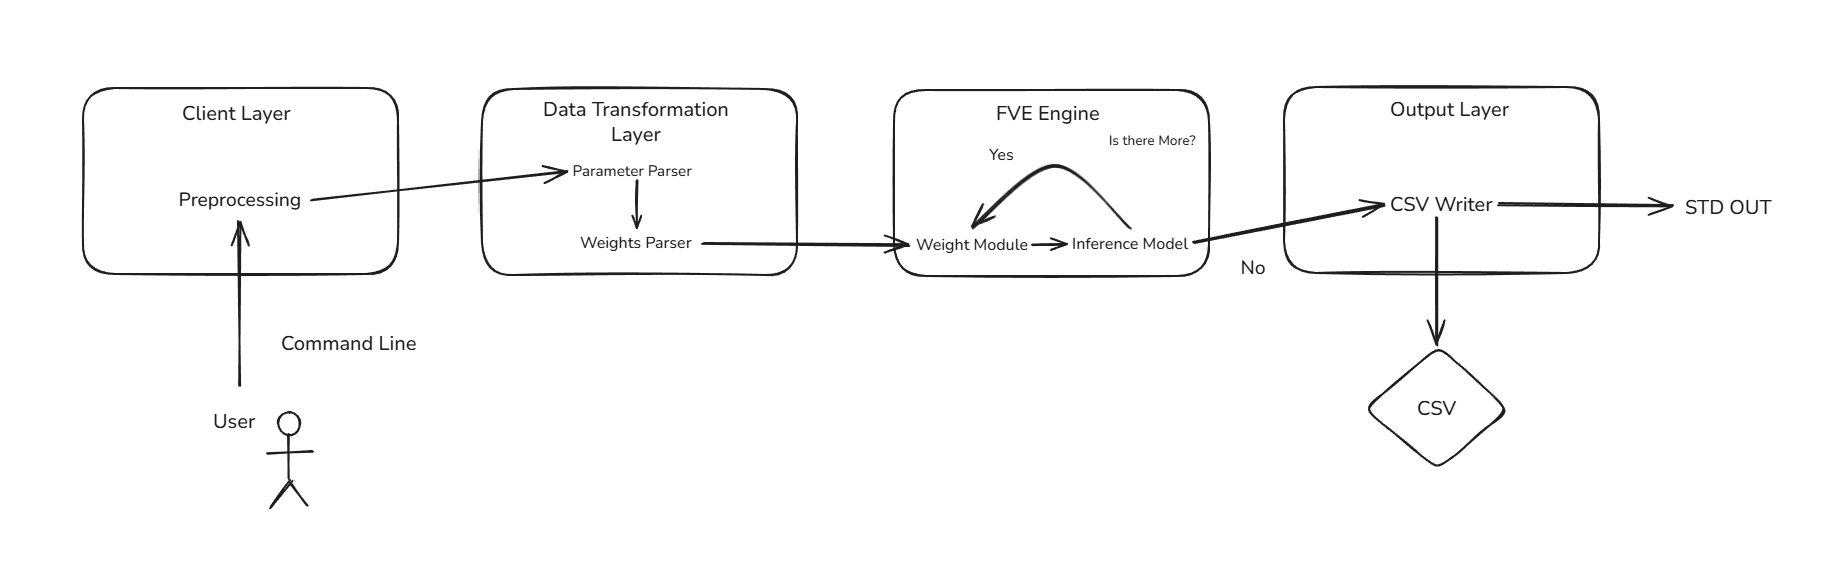
\includegraphics[width=6.5in,height=2.01042in]{./media/63af1a4909c8299032bc64138aee56fe46818dd4.png}

\emph{In this figure, the different components of the system are shown
and how they interact with each other. The user will insert their
respective inputs (through the command line) in the client layer. Then
their data will be processed into tokens in the client and then parsed
in the data transformation layer before going into the FVE Engine. The
FVE Engine is the main determinant where the CMA estimated value will be
generated, depending on the various criteria of rulings to achieve a
better-defined value. The CMA will be constantly looped for any
properties until the batch is complete. Finally, in the output layer,
the CMA will be imported as its output and then applied onto the CSV
file for the result.}

UML Class Diagram

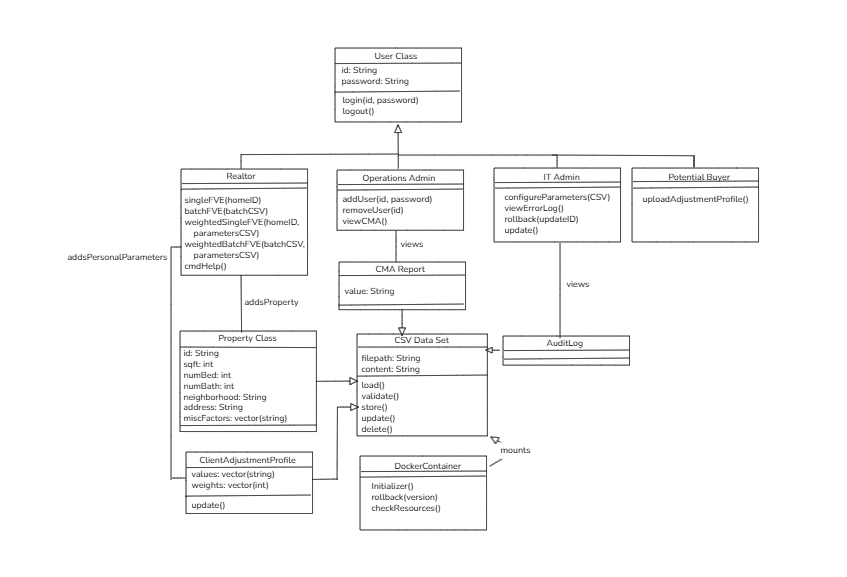
\includegraphics[width=6.5in,height=4.42708in]{./media/176f34dc4097bc3ac3d1d5093927d0cf790ccb35.png}

\emph{Shown are the various user classes and CSV file types, and how
they interact. There are 4 user classes} \emph{: realtor, operations
admin, IT admin, and potential buyer. There are 5 CSV files: the
property class, CMA report, audit log, docker container, and client
adjustment profile.}

Context-level Diagram\\
\strut \\
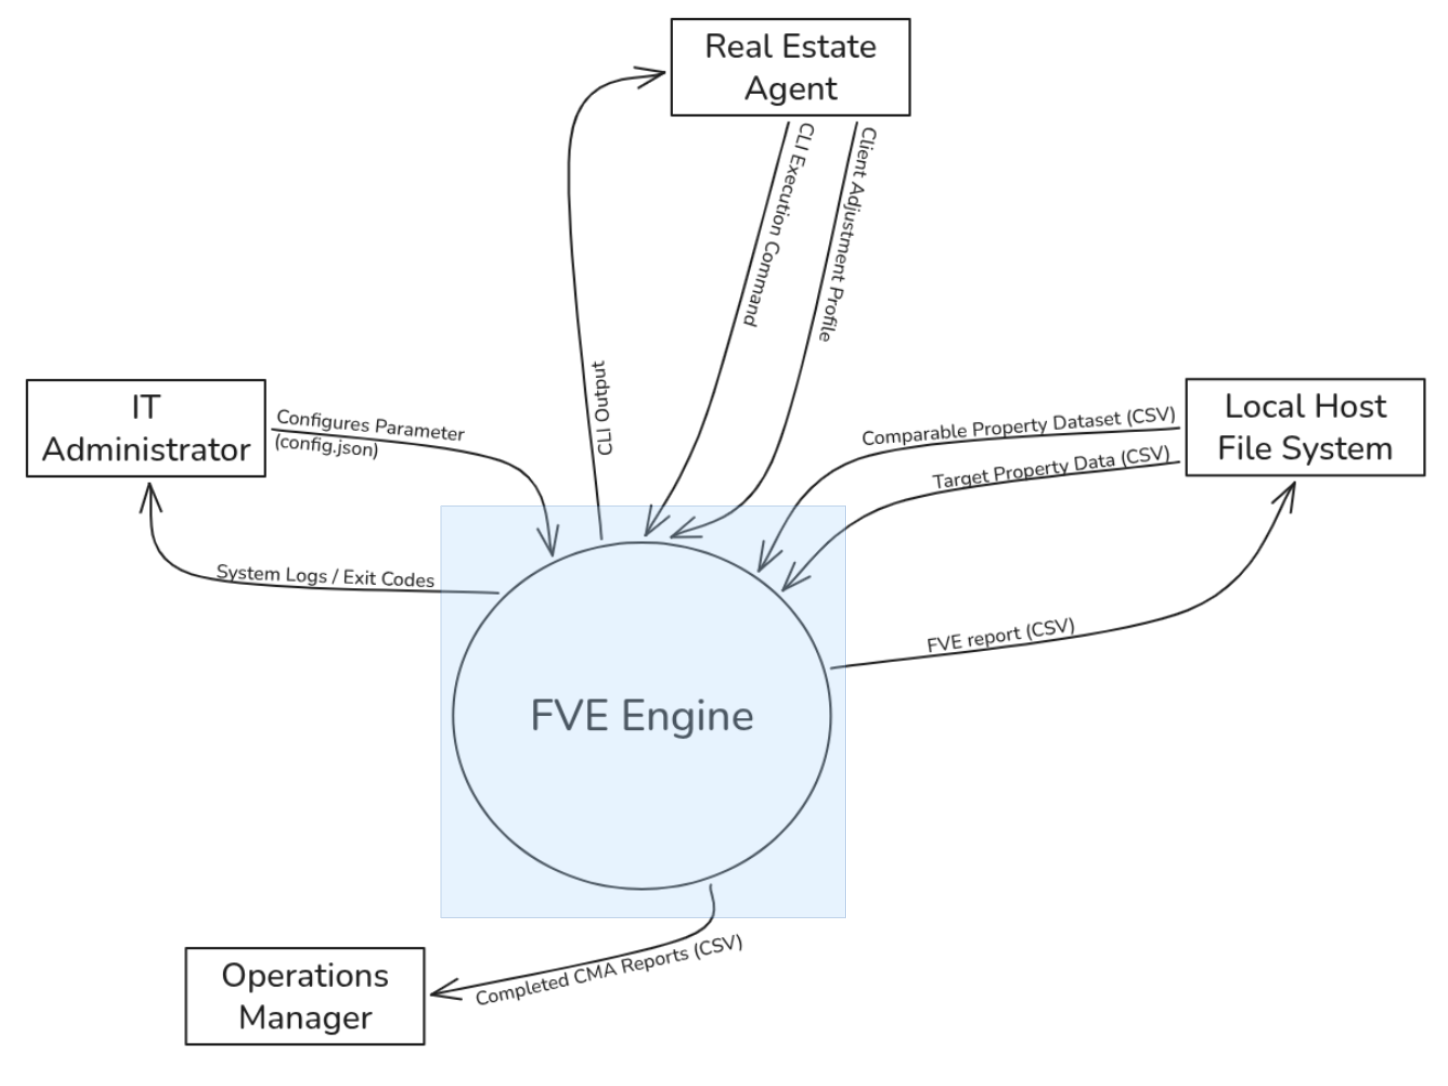
\includegraphics[width=6.5in,height=4.875in]{./media/0307a95bdbc4fe0d81d43496a30ae3310cd7dc1a.png}

\emph{The figures show all of the connections to the FVE Engine. This is
to show how data flows into and out of the FVE Engine. The real estate
agent, the primary users, inputs the adjustment profile of the
individual customer and inputs the execution command. In return, the FVE
outputs the CLI output of the execution. The local host system provides
the dataset of the actual property and comparable datasets to the FVE
Engine. It is given the FVE report in CSV format to be stored in logs.
The IT administrator configures the parameters and receives the exit
codes. The operations manager receives completed CMA reports.}

Data Flow Diagram (1 of 2): Running FVE from start to finish (including
Client Adjustment)

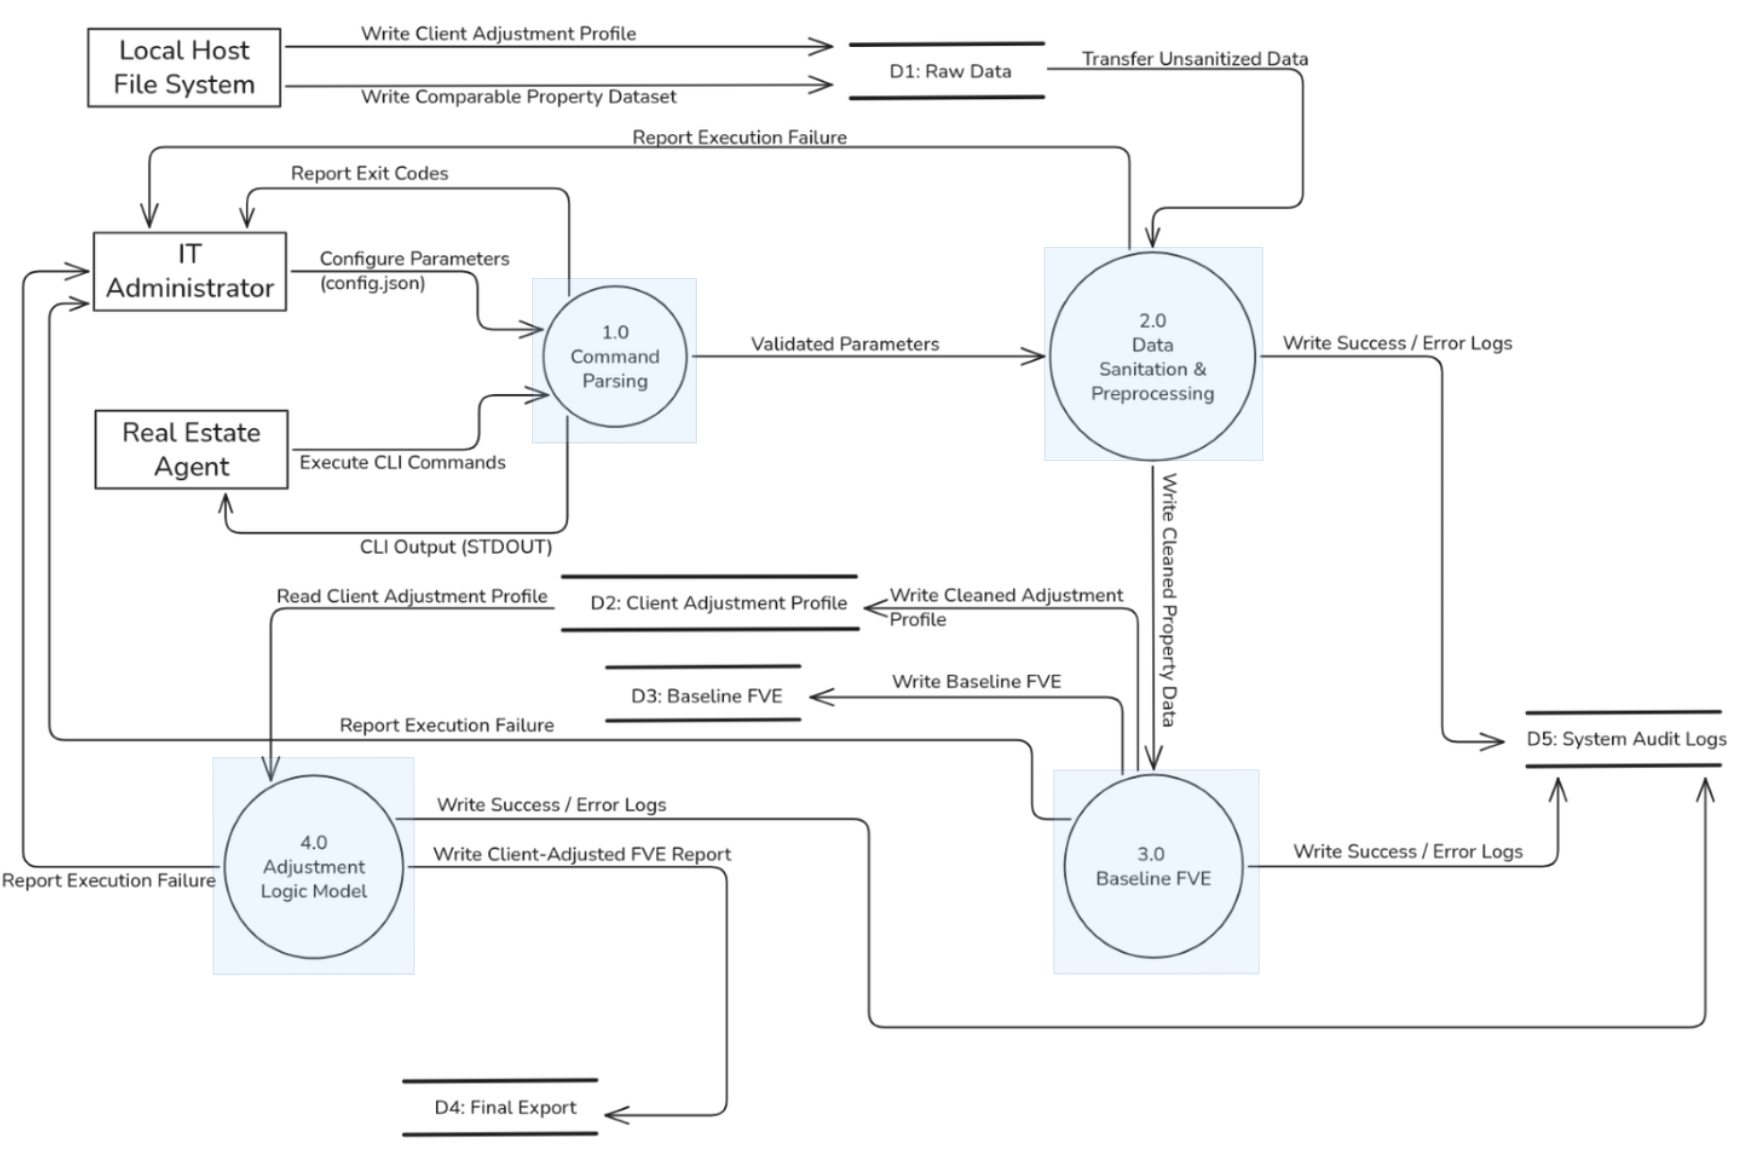
\includegraphics[width=6.5in,height=4.28125in]{./media/ae5bc5ea3f3142667f69fd217e929fbeb924ef22.png}
\emph{D1-D4 represents sub directories within the database and has been
explicitly stated for added clarity for the data flow diagram.}

\emph{For the figure, the FVE Engine is clearer with better data flow
interaction amongst how the actors of the Local Host, IT Administrator,
and the Real Estate Agent are interacting. The Local Host is inputting
the original file for raw data to be processed. The IT Administrator
ensures configuration parameters through config.json as well as
receiving any execution code failure reports from the transmitted
processing operation. The Real Estate Agent may execute CLi commands to
parse and retrieve the output through STDOUT.}

\emph{For each central processes, it helps perform the following:}

\begin{itemize}
\item
  \emph{1.0 deals with command parsing through CLI commands from the
  Real Estate Agent and configuring parameters from the IT
  Administrator. These inputs are taken and are validated to be
  processed to 2.0 .}
\item
  \emph{2.0 will take in the validated parameters and the original, raw
  data to return its property data to 3.0 and transfers its clean
  profile to D2. Any other log successes or failures throughout the
  process will be navigated to D5.}
\item
  \emph{3.0 is the baseline for FVE where it takes 2.0 cleaned property
  and operates the calculations. The output will be passed to 4.0 and
  other FVE write baselines to D3. Any other errors or failures logged
  will be passed to D5.}
\item
  \emph{4.0 operation would take in D2's profile returns and applies its
  client-specific adjustment logically models to its finalized FVE
  report. This report will be passed to D4, any written model logged
  failures or successes will go to D5, and the execution of failures be
  passed to the IT Administrator.}
\end{itemize}

Level-1 Data Flow Diagram (2 of 2): Running Client Adjustment on
preexisting properties with prior FVE

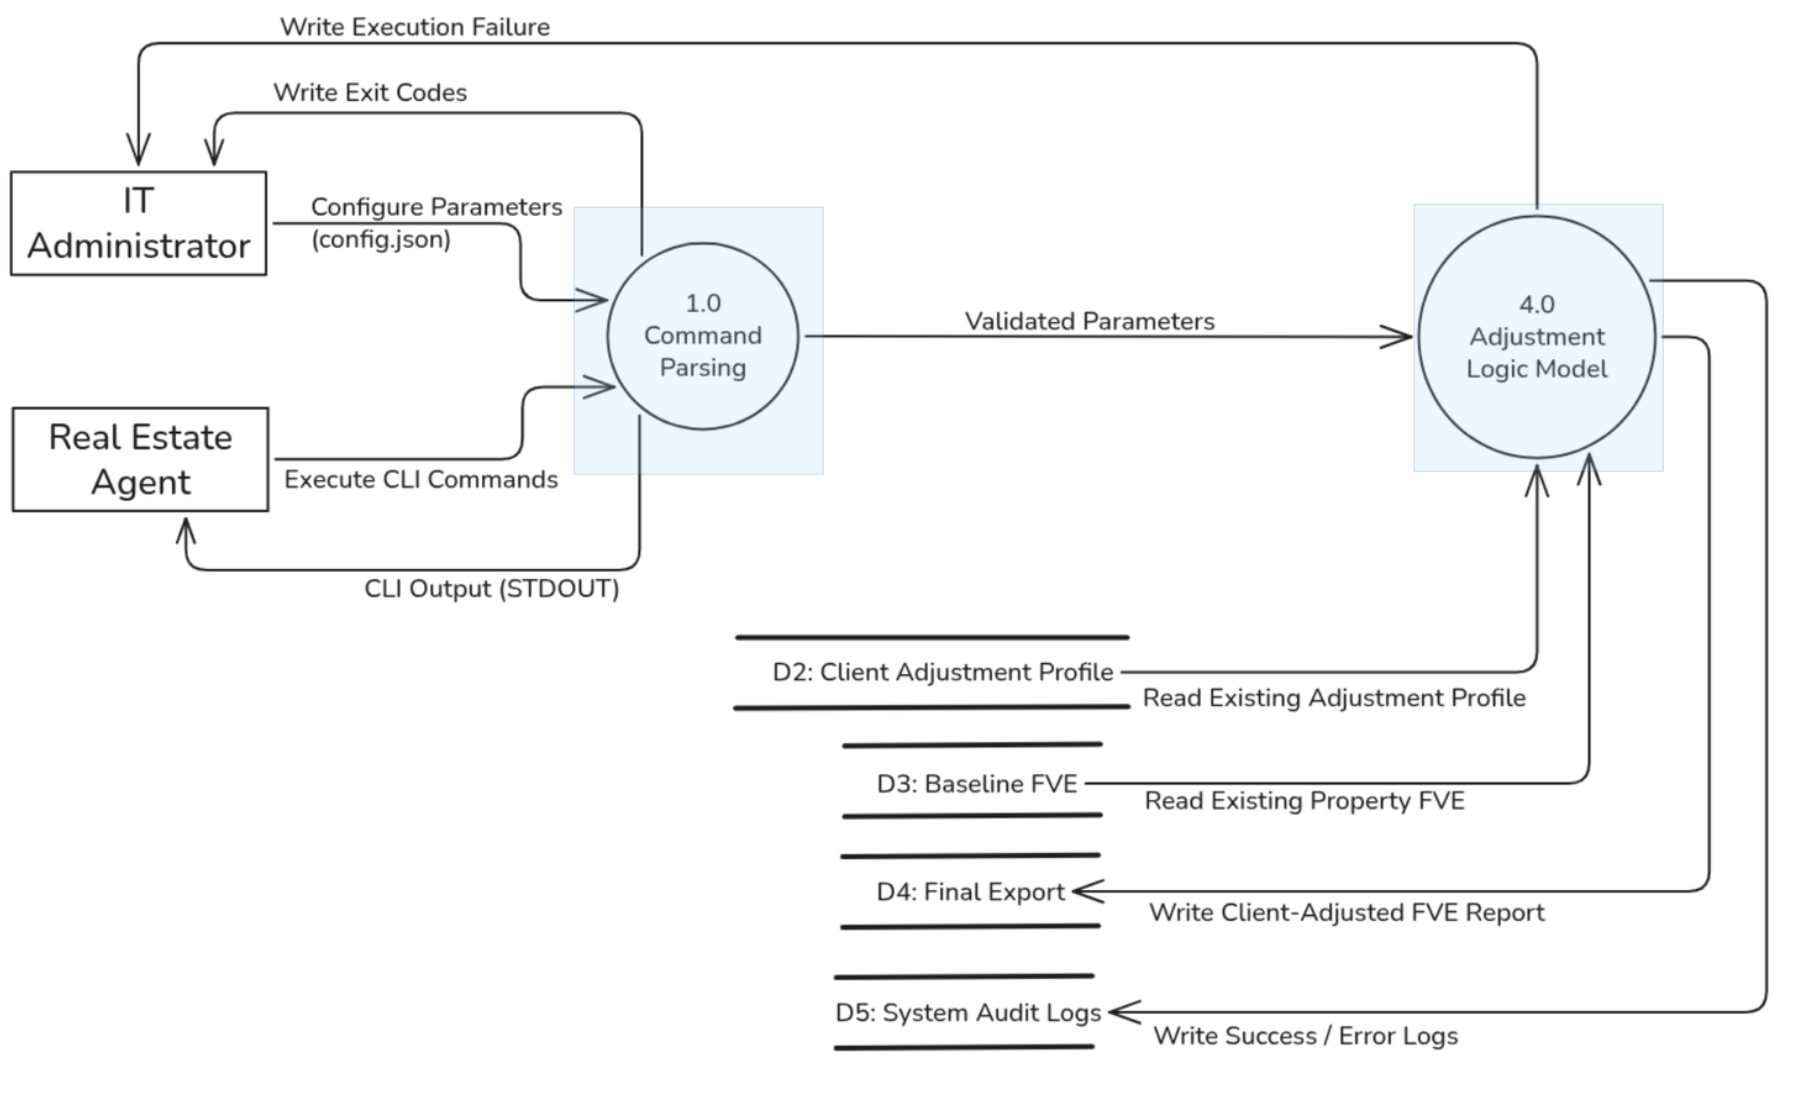
\includegraphics[width=6.5in,height=3.97917in]{./media/d54706cfd22234abe060f52b9e4d4e1404e3a29c.png}

\emph{This figure shows a different approach where pre-existing data
properties are already present for the FVE Engine to operate. The IT
Administrator and Real Estate will pass their respective configuration
parameters and CLI Commands to 1.0 as before. However, the validated
paramaters will now be sent directly to 4.0 ALM. With the ALM's given
pre-existing data, the logic will read existing profiles already given
from D2 and D3 FVE baseline properties. The ALM will perform the same
operation and write its finalized report to D4 and logging it to D5. Any
execution of failures or errors will be written to the IT
Administrator.}

Level-2 Data Flow Diagram (1 of 3): Data Sanitation \& Preprocessing
Process

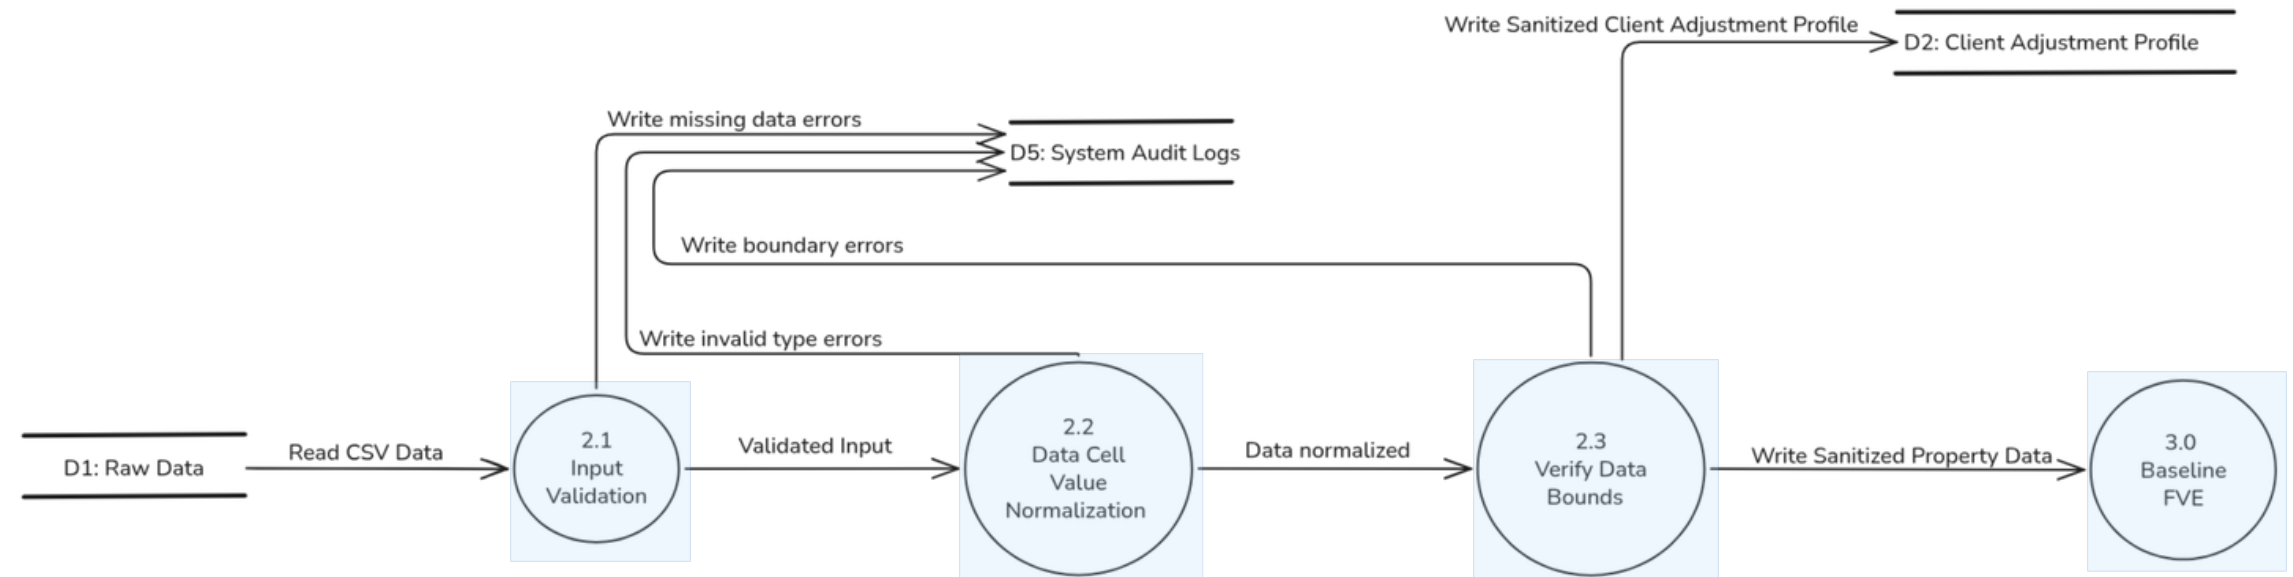
\includegraphics[width=6.5in,height=1.63542in]{./media/a69c75f357bd16ee10a9bf78d863c7d7e242f66e.png}
\emph{The figure dives into the Baseline FVE Process and how its
sub-directories processes are sanitized and processed from 2.0. The raw
data gets passed into 2.1 - 2.3, where each operation is checked for any
boundary errors, invalid input criteria\textquotesingle s, and missing
data that\textquotesingle s necessary to proceed. Each operation will be
first validated, normalized, and then verified to ensure that 2.0's core
functionality will be sanitized and standardized to be passed to 3.0.
Any raw data that violates the errors will be directly sent to D5. For
2.3, its outputs will be judged and redirected to D2 for written
sanitized client adjustment profile or its sanitized property data be
passed to 3.0.}

Level-2 Data Flow Diagram (2 of 3): Baseline FVE Process

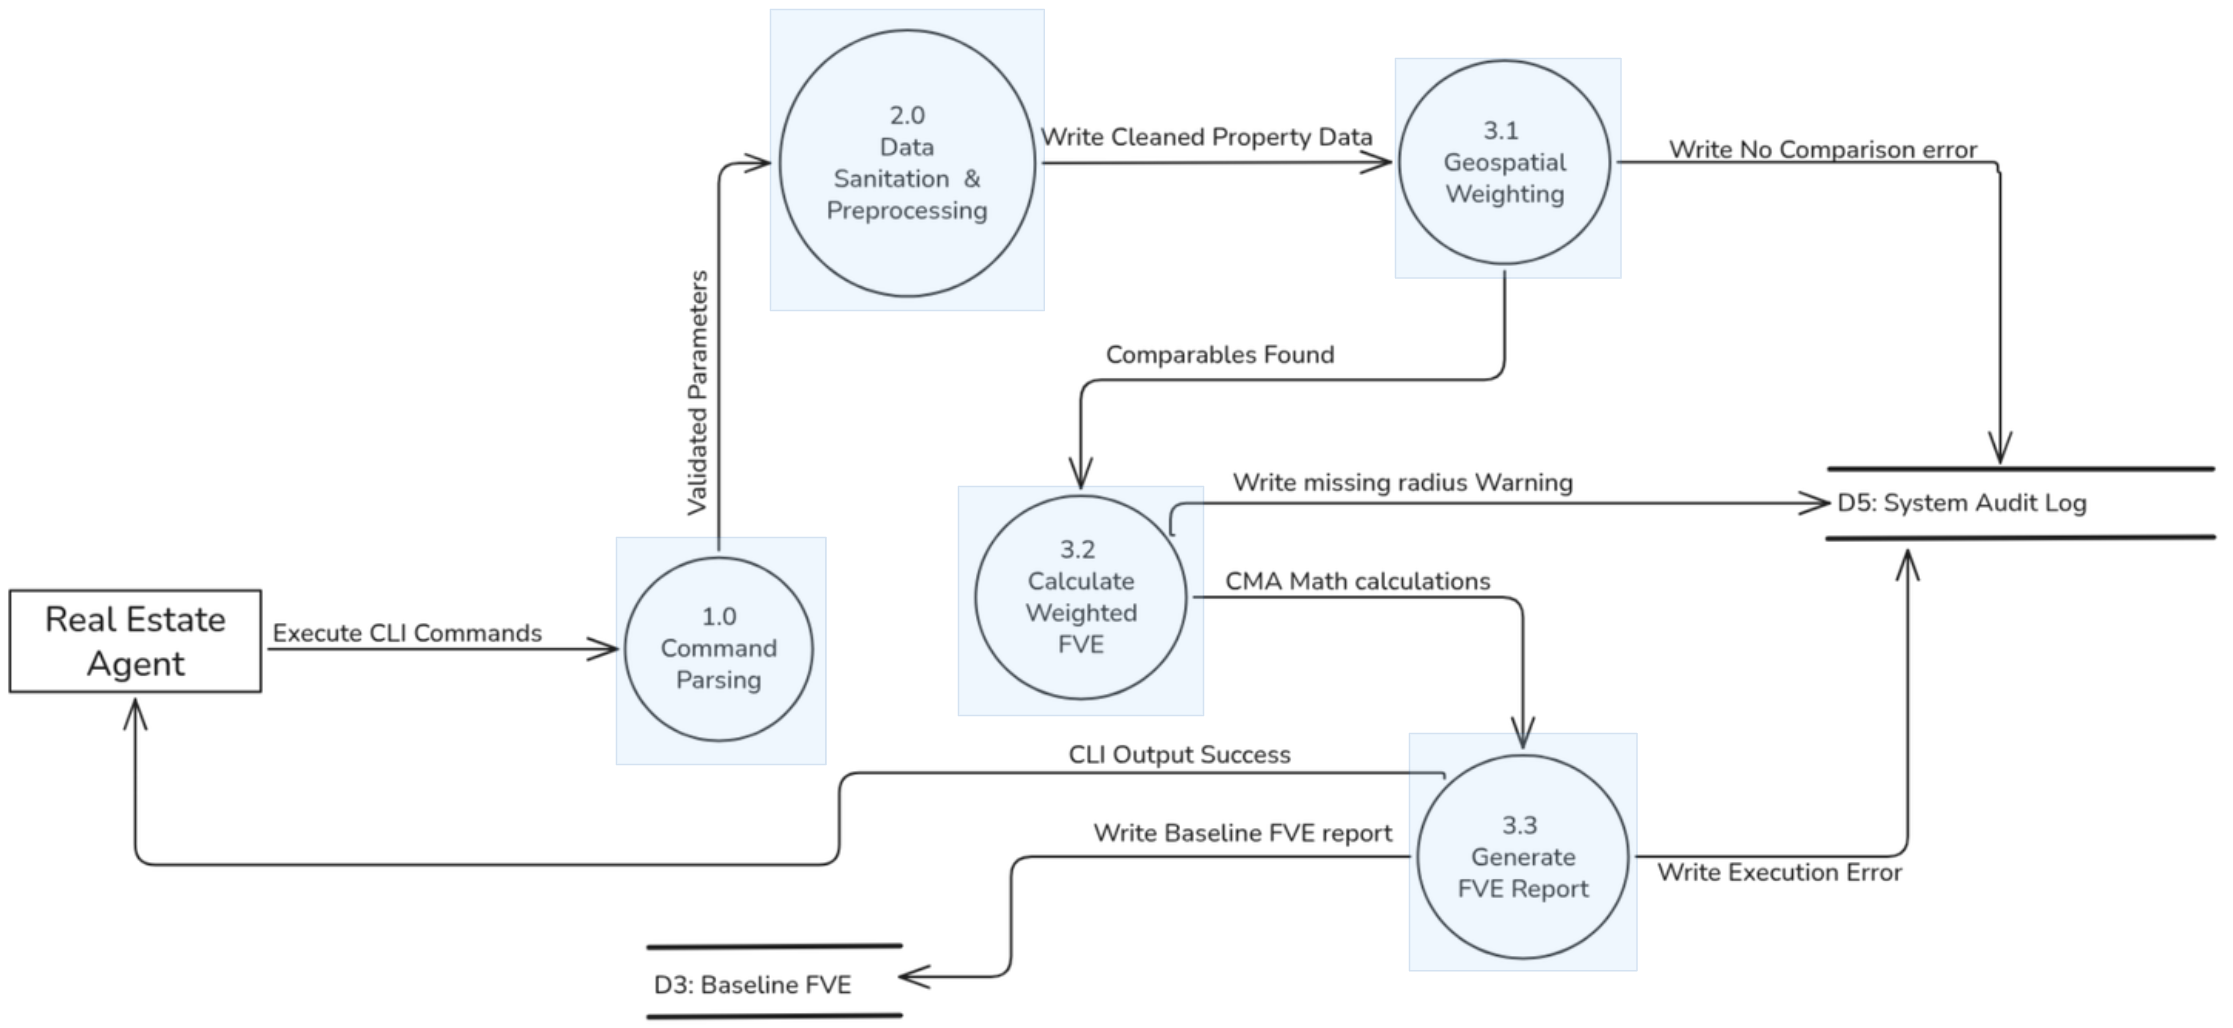
\includegraphics[width=6.5in,height=2.98958in]{./media/f3ab85f093e70f4c3eb2d8a697273a0114c22e98.png}

\emph{The figure deals with 3.0 for its Baseline FVE Process. After 2.0,
its cleansed property data will be redirected to 3.0. The geospatial
weighting will be first encountered, where it weighs various comparable
properties that the geographic criteria are applied onto. Such
comparable properties found will be passed to 3.2 while any missing will
be sent to D5. 3.2 will read the parsing comparable and weighted data
and run the CMA calculations to get an output. If the radius goes
missing for any comparable calculations, write it to D5. Otherwise, the
calculations will be passed to 3.3. The final step for 3.3 will take in
the CMA calculations and produce the FVE. Upon success, it will write
the FVE report to D3 or D5 if the execution was unsuccessful.}

Level-2 Data Flow Diagram (3 of 3): Adjustment Logic Model Process

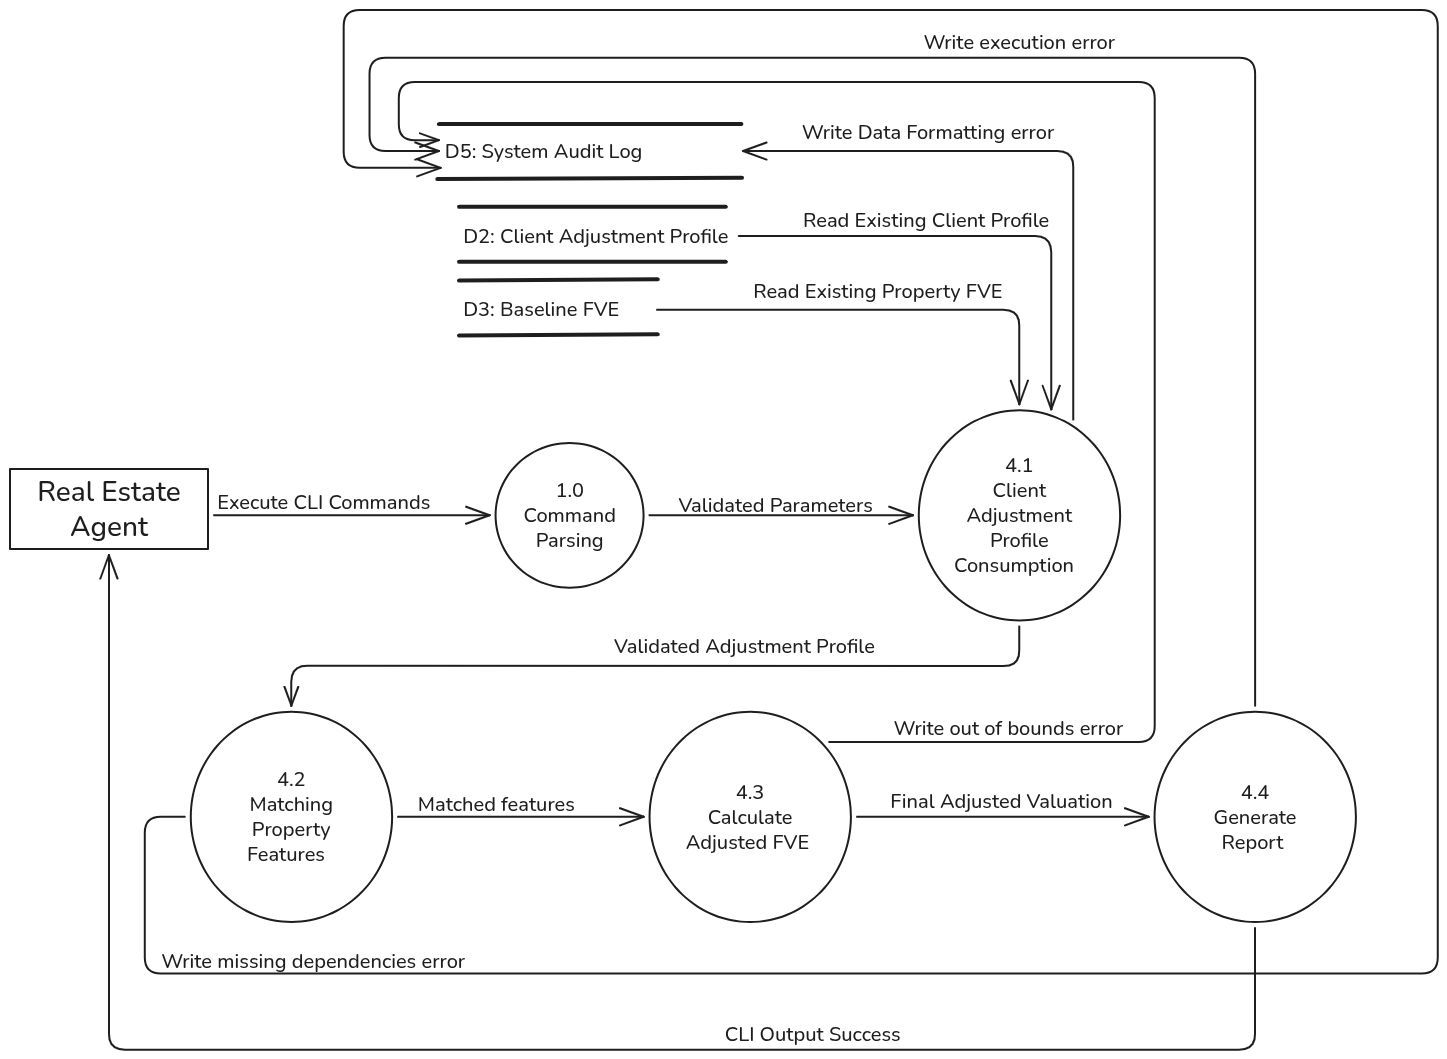
\includegraphics[width=6.5in,height=4.76042in]{./media/c097d84af31d80ab5bb4526444b8910243fa7b72.png}
\emph{The figure dives deeper into 4.0, where the diagram shows 4
different sub-sections for processing. For 4.1, it retrieves all 3
sources from the Real Estate Agent, D2, and D3 to validate and merge all
information into a CAP. This profile will be passed to 4.2 while any
formatting pathway errors are dragged to D5. Sub-section 4.2 takes the
whole CAP and matches each user\textquotesingle s subject property
features, which upon succession will be passed to 4.3. Any missing
dependencies found from matching calculations will be audited on D5. For
sub-section 4.3, the matched features will be applied to the adjustment
logic to compute the FAV and be transferred to 4.4 to generates it
outputted report and send it to the Real Estate Agent. Any boundary or
execution issues arising from these sub-sections will be reported back
to D5.}

Use Case Diagram

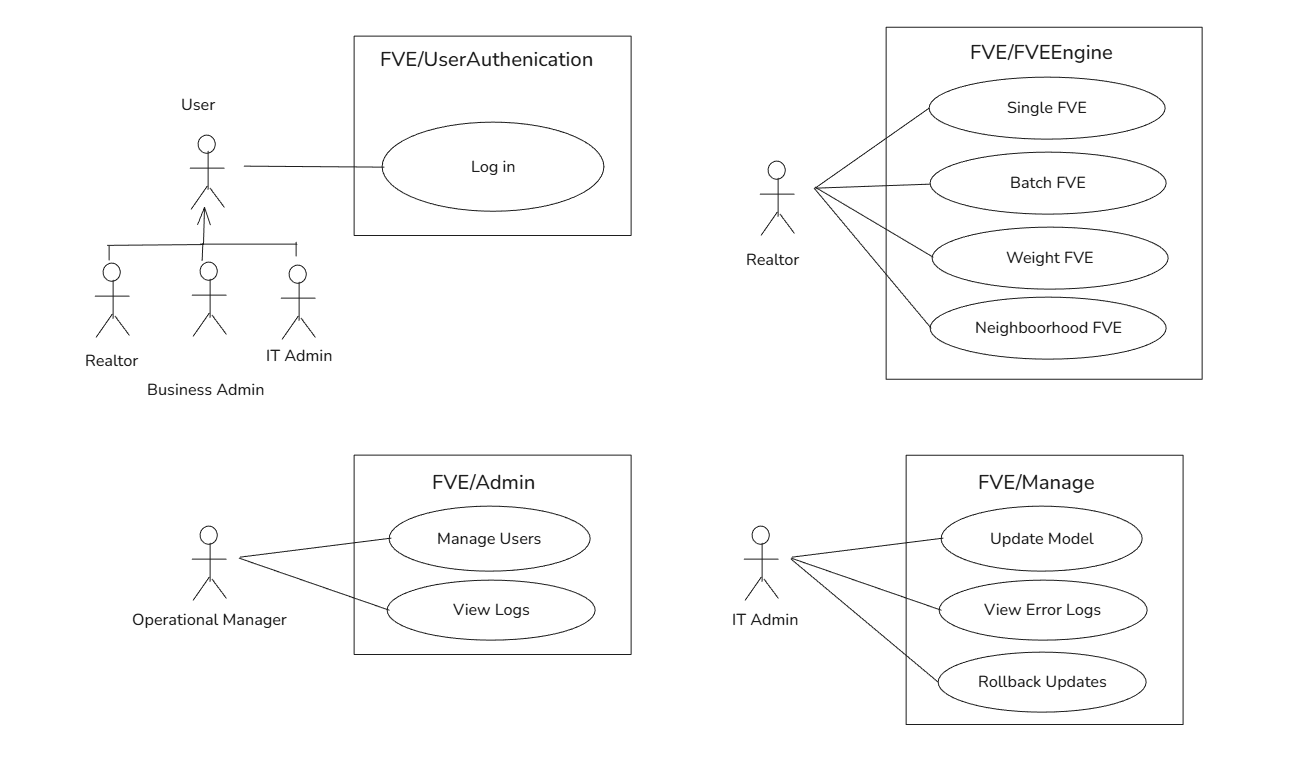
\includegraphics[width=6.5in,height=3.90625in]{./media/1f78ca3768b1c777707606b1f80919ce6d091ae2.png}

\emph{The figures dive into the primary actors that are interacting with
the Fair Value Estimate (FVE) and the specific actions they are
authorized to perform within those actions. First the Fve/user
authenticator creates a base level of access to the system through a log
in function. This base layered pathway is then inherited by the systems
three sub-actors the realtor, business admin and the IT admin. The
diagram then branches into role specific capabilities, showing the
realtor interacting directly with the FVE. Within this module, the
realtor is allowed to execute core processes specifically a single FVE,
a Batch FVE, weight FVE and a neighborhood FVE. The Operational Manager
accesses the FVE/Admin module. This section grants the manager
administrative privileges to Manage Users and View Logs. Finally, the IT
Admin interacts with the FVE/Manage module to handle system maintenance.
Through this module, the IT Admin is authorized to perform technical
support tasks, including the ability to Update Model, View Error Logs,
and Rollback Updates.}

\phantomsection \phantomsection\section{9. Detailed System Design}\label{detailed-system-design}

\phantomsection \phantomsection\subsubsection{Log in screens and
menus:}\label{log-in-screens-and-menus}

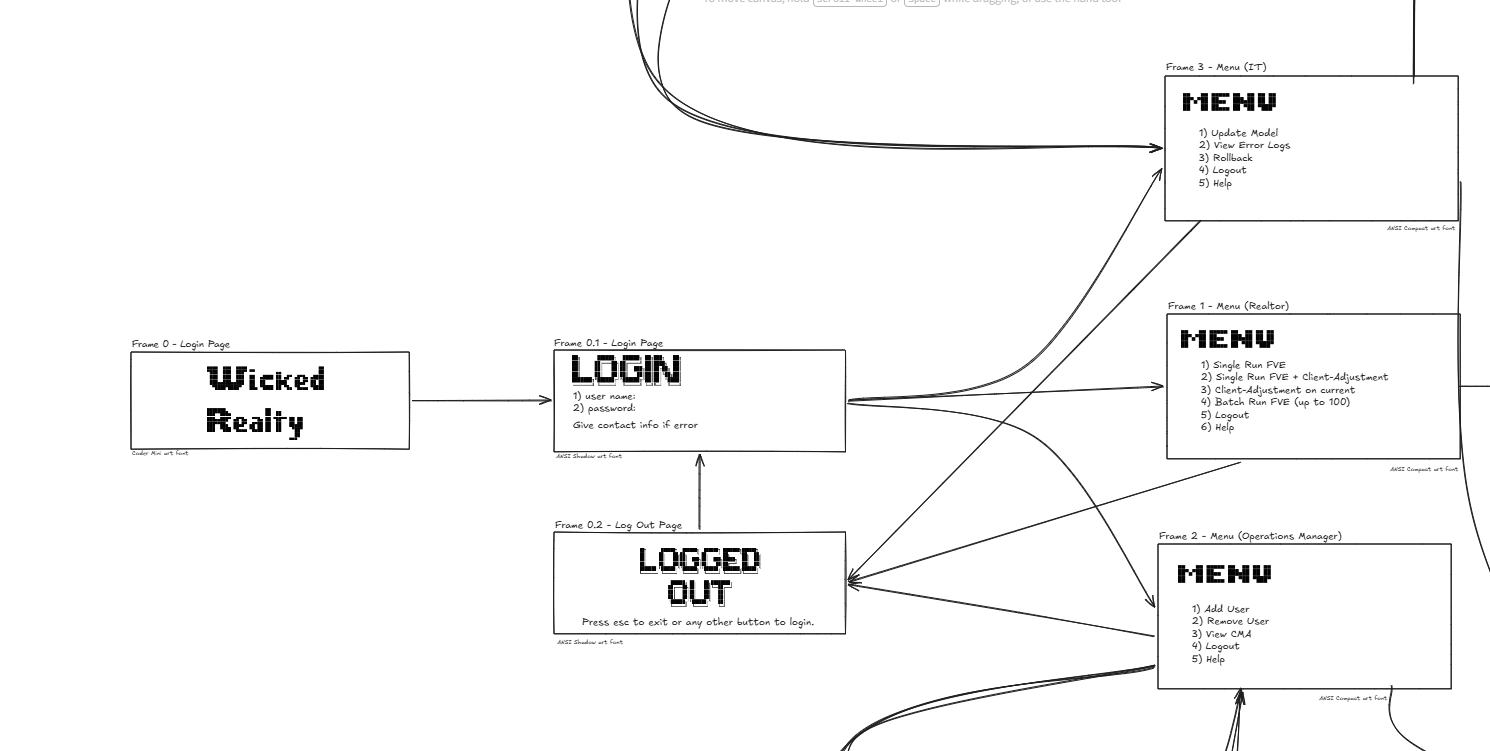
\includegraphics[width=6.5in,height=3.28125in]{./media/8c121b8789bbf6f1b2bea30be3e115f7c8258576.png}\emph{This
is a prototype of the login screens shown to the client. It features a
title screen, a login screen, a menu screen for each role, and a log-out
screen. These would all be in the command line, as mentioned in System
Feature 2: CLI application, for ease of use, as would every other screen
shown in the prototype.}

\hypertarget{realtor-screens}{%
\subsubsection[Realtor Screens: ]{\texorpdfstring{Realtor Screens:
\protect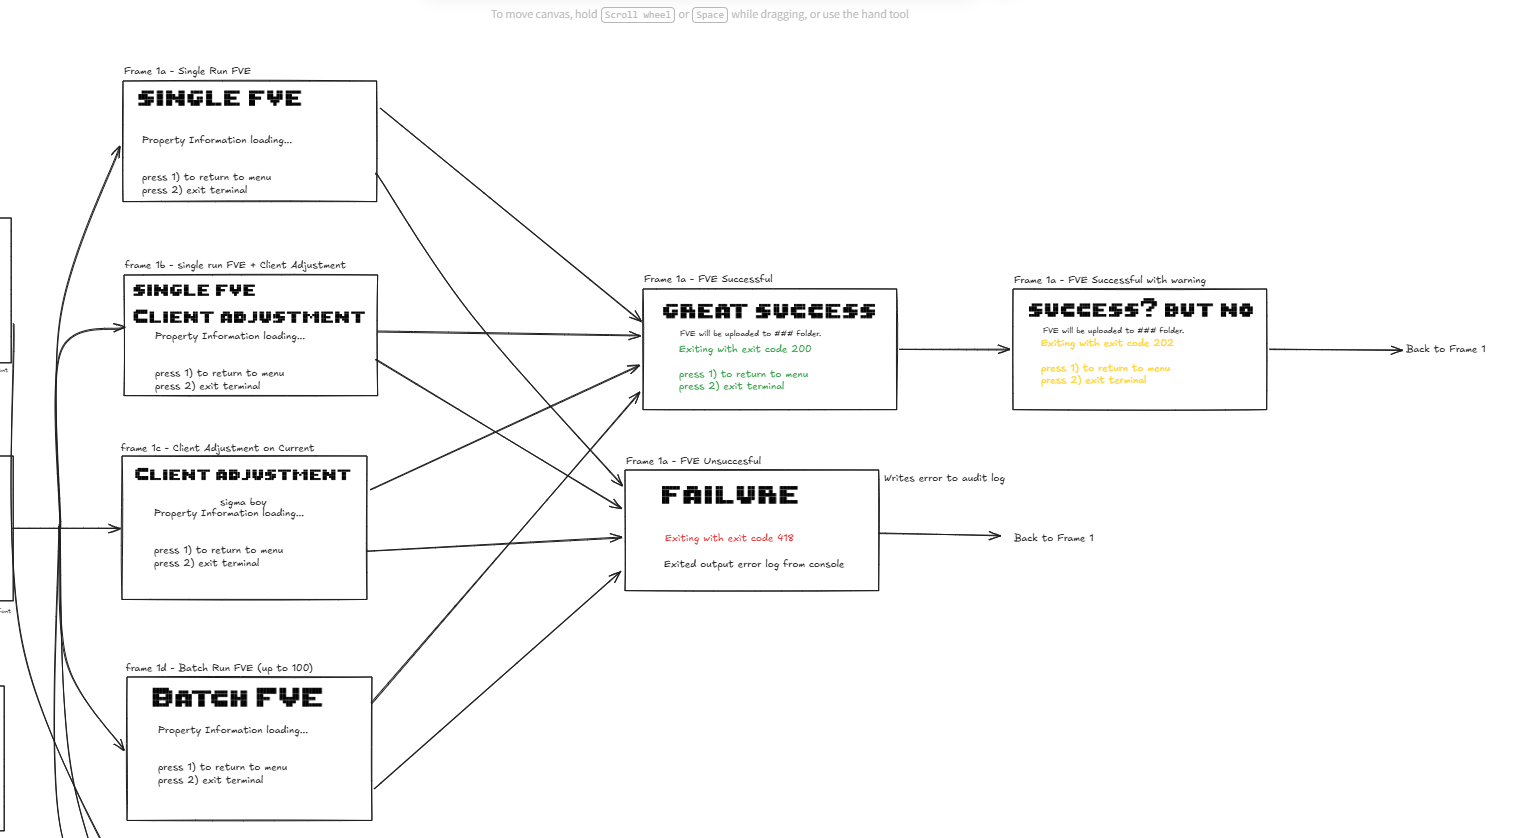
\includegraphics[width=6.5in,height=3.58333in]{./media/e6b1abc6365357ef8a7befb04c0034c074bad9e6.png}}{Realtor Screens: }}\label{realtor-screens}}

\emph{Here are the different options for the realtors on the same
prototype. The realtor would be able to run a single FVE, a single FVE
adjusted for the client, or a batch FVE. To do this, the user would
upload a CSV into the INPUT\_FILES\_HERE folder, and if adjustments were
necessary, they would upload a CSV to the ADJUSTMENTS folder, as per the
requirements of System Feature 6, Local Data Collection and Storage, and
System Feature 5, Adjustment Logic Model. In the background, the data
would then be processed and parsed as per System Feature 3, Data
Sanitation and Preprocessing. Afterwords the FVE engine would calculate
the FVE, as said in System Feature 4, FVE Engine. This would store the
CSV in an output folder accessible to the realtor, as noted in System
Feature 6, Local Data Collection and Storage. These would all lead to a
success screen or a failure screen. As mentioned before, this would all
be done in the CLI as per System Feature 2, CLI application.}

\hypertarget{it-screens}{%
\phantomsection\subsubsection{\texorpdfstring{IT Screens:
}{IT Screens: }}\label{it-screens}}

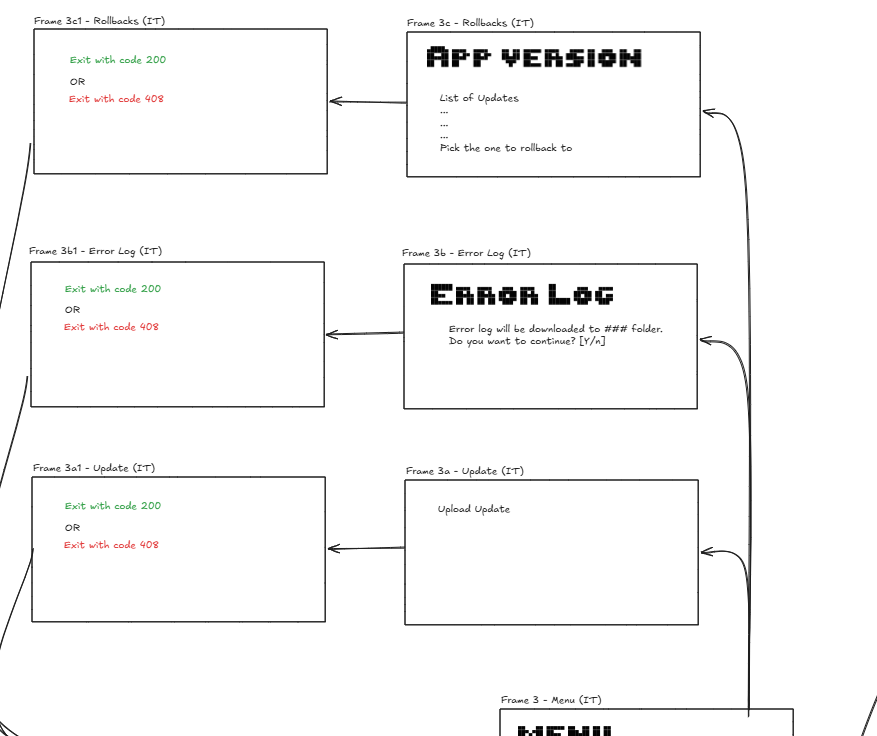
\includegraphics[width=6.5in,height=5.45833in]{./media/ef561d1aac062d9a60c028db210e18c89de98819.png}

\emph{The IT admin screens are the app version, error log, and an upload
update screen in the prototype. The error log was the most important, as
any failures would be recorded there and output to an error log CSV, as
per System Feature 6, Local Data Collection and Storage.}

\hypertarget{operations-manager-screens}{%
\phantomsection\subsubsection{\texorpdfstring{Operations Manager Screens:
}{Operations Manager Screens: }}\label{operations-manager-screens}}

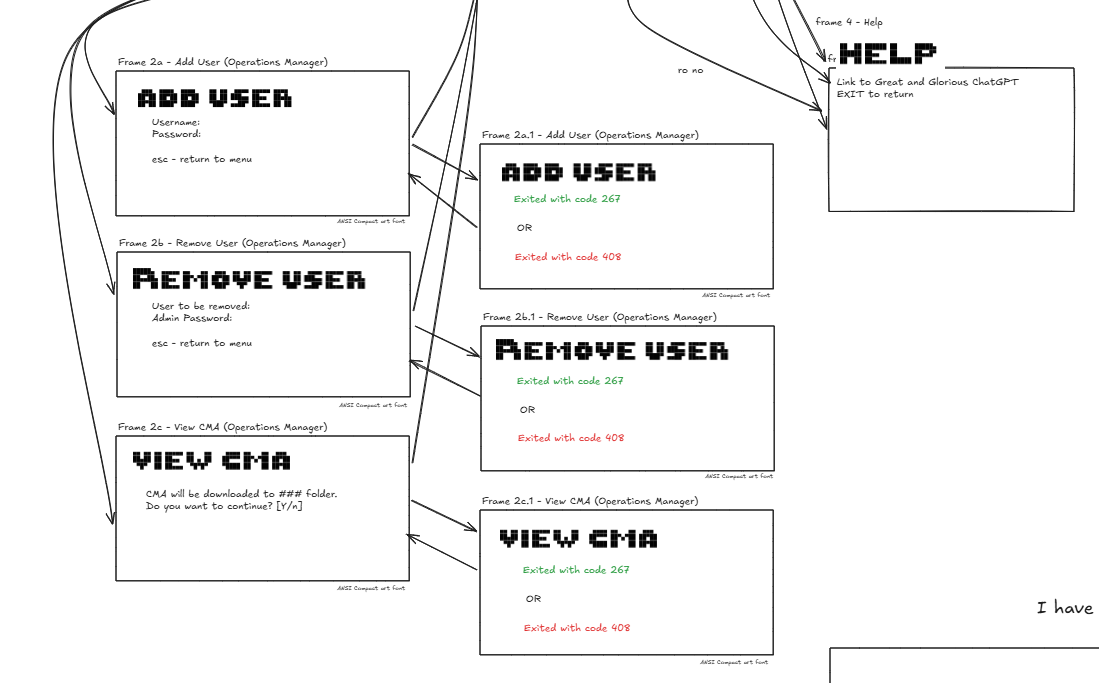
\includegraphics[width=6.5in,height=4.04167in]{./media/0ff85bba1d3076d70b92656d72a8ae792c9ca56e.png}

\emph{Operations Manager screens in the prototype show Add and Remove
Users and View the CMA. The CMA would be viewed locally on a CSV as per
System Feature 6, Local Data Collection and Storage.}

\hypertarget{overall-diagram}{%
\phantomsection\subsubsection{\texorpdfstring{Overall Diagram:
}{Overall Diagram: }}\label{overall-diagram}}

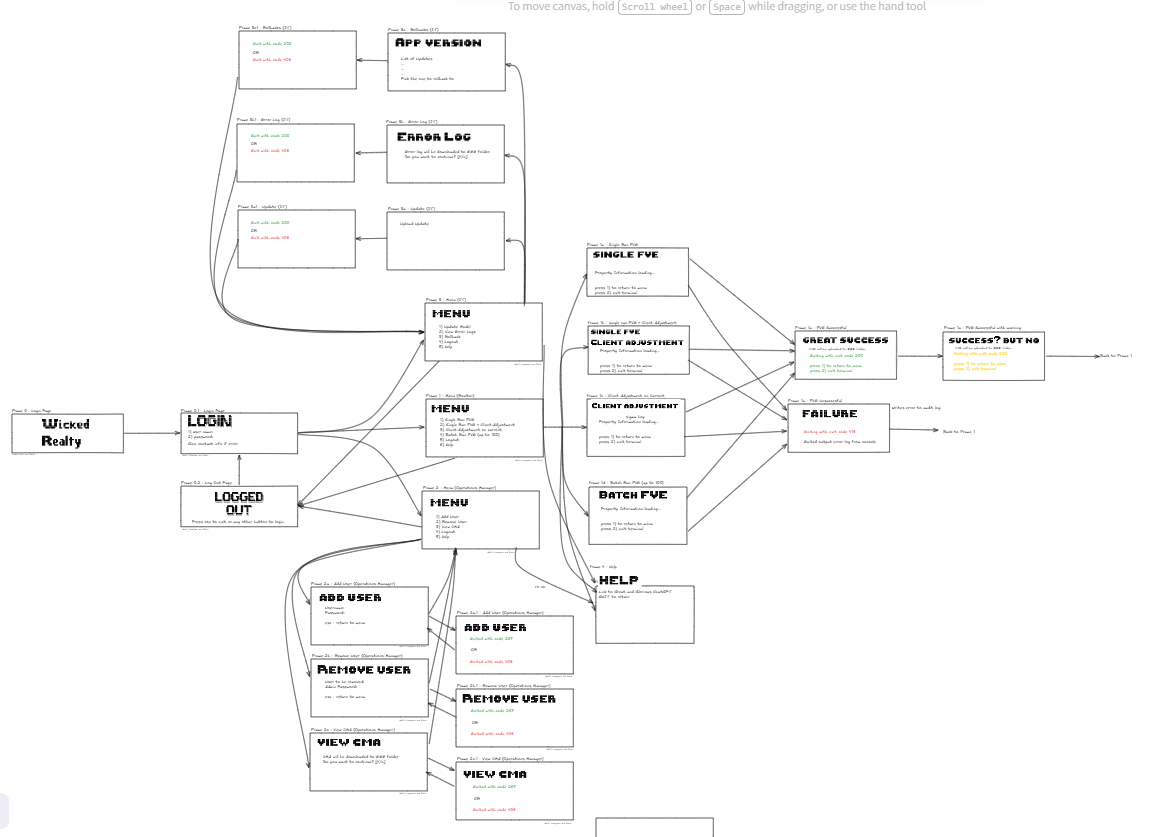
\includegraphics[width=6.5in,height=4.65625in]{./media/021b759754c80bd60fb9e6fdfb24f8b54e2929f7.png}

\emph{Here is a fully zoomed-out diagram of the UI prototype and all of
its screens to give a better picture of the full application and how any
user could navigate the app. All of the screens would be shown in the
CLI, as per System Feature 2, CLI application.}

\phantomsection \phantomsection\subsubsection{Hardware, Software, and Communication
Interfaces}\label{hardware-software-and-communication-interfaces}

To create this CLI interface, Ink's library will be used. This allows
for the screens with colors and fonts to indicate visually successes,
failures, and errors. In addition, we xterm-256color was chosen as the
emulator of choice within each docker container to render the ink
colors.

Hardware Interface: T

ested on NUC11PAHi7 with 16 gb of RAM, though any device that can run
docker should suffice.

Disk Space: 100mb not including docker.

Software Interface:

A docker compose file is provided alongside a Docker file to build and
update the container. Update deployments can be run within the container
via a simple git pull and revert with git. The docker compose file
houses several volumes; of note are the following: FVE\_OUTPUT,
DATASET,INPUT FILES, TMP, ERROR\_LOGS, config.json, adjustments.json,
users.json, roles.json/. This allows the container to retain any
important files as persistent memory in the event of a container
crashing or container being brought down.

OS:

Any OS compatible with downloading Docker and running the container. For
development, prefer Ubuntu 24.04. If the client wishes, upon additional
fee an ansible image may be setup per each operating system for ease of
modification, though currently is not provided due to the user side of
the application being done purely through docker.

Remote asceses:

To test remote access, we used an internal tailnet with the same ports
as defined in the docker file. We then connected via another pc to the
said device running the container at the given port in the docker file.
The UI was made with ttyd and ported to the docker port which appeared
on devices web url. However, as previously stated, a full tailnet can be
provided upon an additional contract fee and discussion and is assumed
to be already within the client's system.

Runtime Environment:

Node.js 16 inside of Docker

Dependencies: as listed in my-cli/package*.json\\
"csv-parse": "\^{}6.2.1",

"csv-stringify": "\^{}6.7.0",

"ink": "\^{}5.2.1",

"ink-select-input": "\^{}6.2.0",

"ink-spinner": "\^{}5.0.0",

"ink-text-input": "\^{}6.0.0",

"meow": "\^{}11.0.0",

"react": "\^{}18.2.0"

\phantomsection \phantomsection\section{10. RD 3.0: More Diagrams}\label{rd-3.0-more-diagrams}

To preface this section, most of the diagrams were created before or
during the creation of the FVE engine. Because of this, the sequence
diagrams and much of the other diagrams were based on the prototype
rather than the final application. This led to some discrepancies in
classes and overall data flow between the diagrams and the application.
Anything that does not match the application should match the prototype.

\phantomsection \phantomsection\subsection{10.1 Sequence Diagrams}\label{sequence-diagrams}

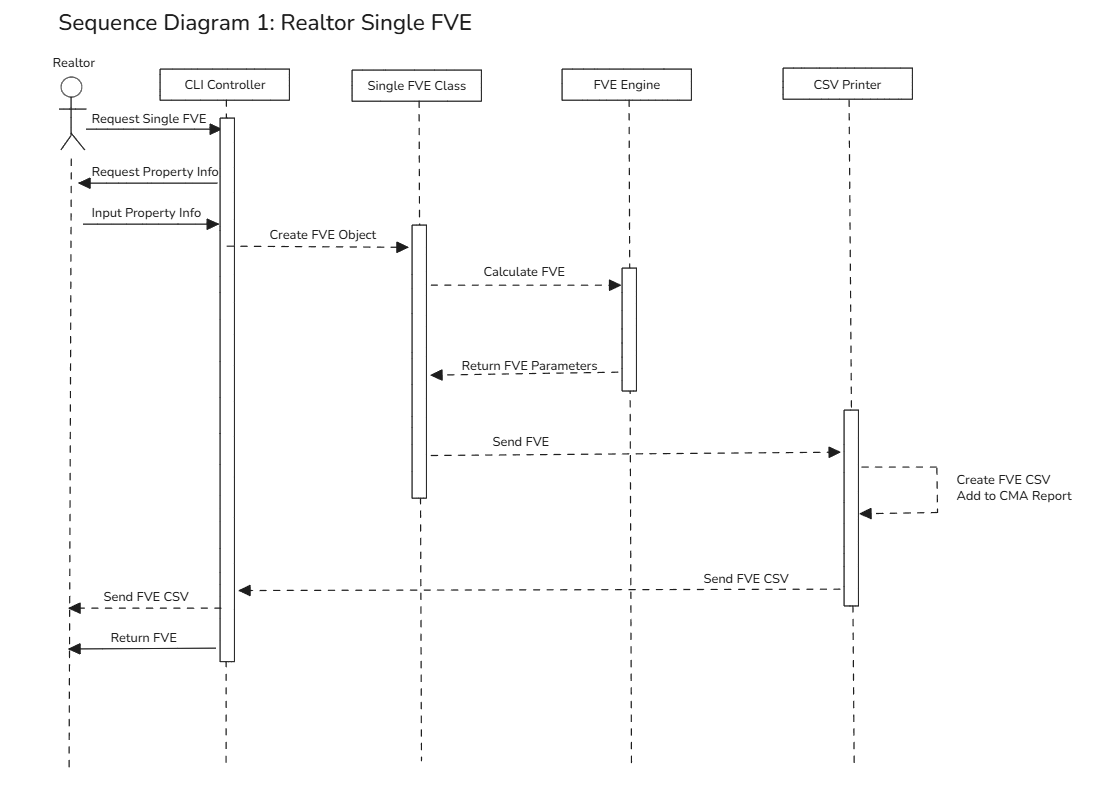
\includegraphics[width=5.48958in,height=3.89725in]{./media/0cf214900af8d6a3f97c97ba84be4c2ac890ba54.png}

\emph{Here is a sequence diagram of the realtor single FVE. This shows
how the classes interact with each other to calculate the single FVE.
First, the realtor inputs the CSV, which is brought to the FVE engine,
where the FVE is calculated. This is added to the CMA report, then
turned into a CSV. This is put into an output folder for the realtors to
access.}

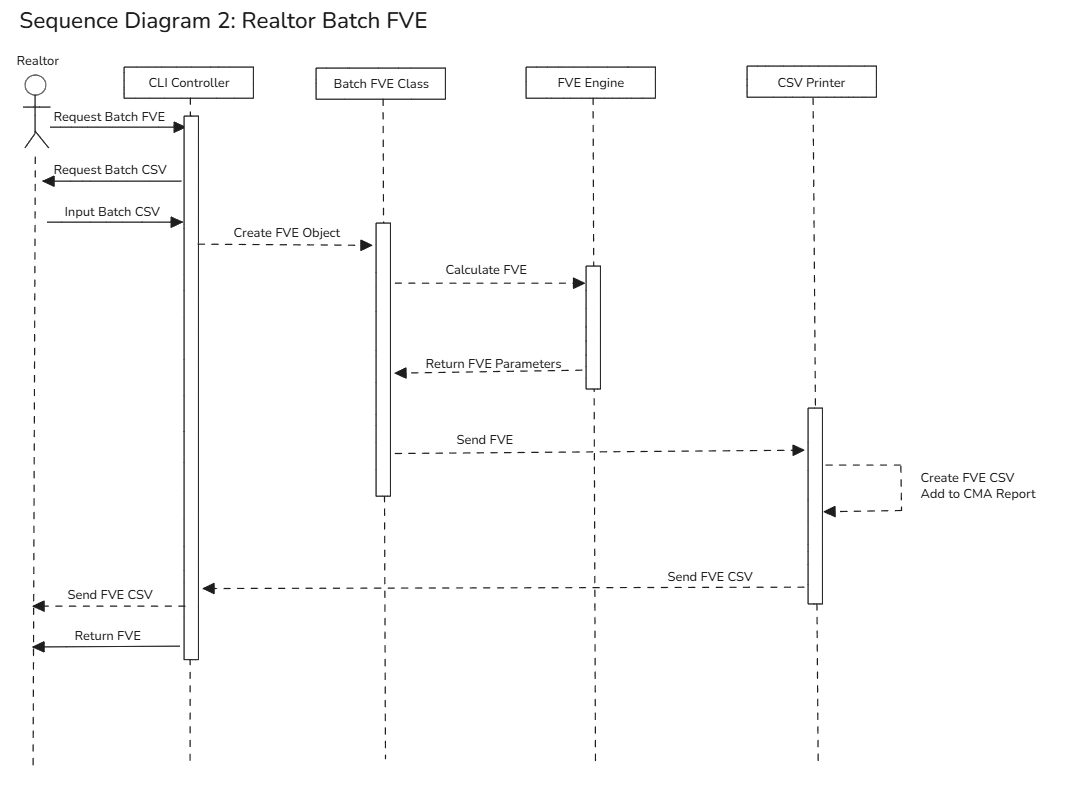
\includegraphics[width=5.66667in,height=4.24092in]{./media/4f0826b8df4812252dbfd5b26888822126aeb5ae.png}

\emph{This is the sequence diagram of a batch FVE. It works mostly the
same as the single FVE. The realtors input a CSV of the properties,
which the engine then calculates all the FVEs. This is written to the
CMA, then written to a CSV in an output folder that the realtors can
use.}

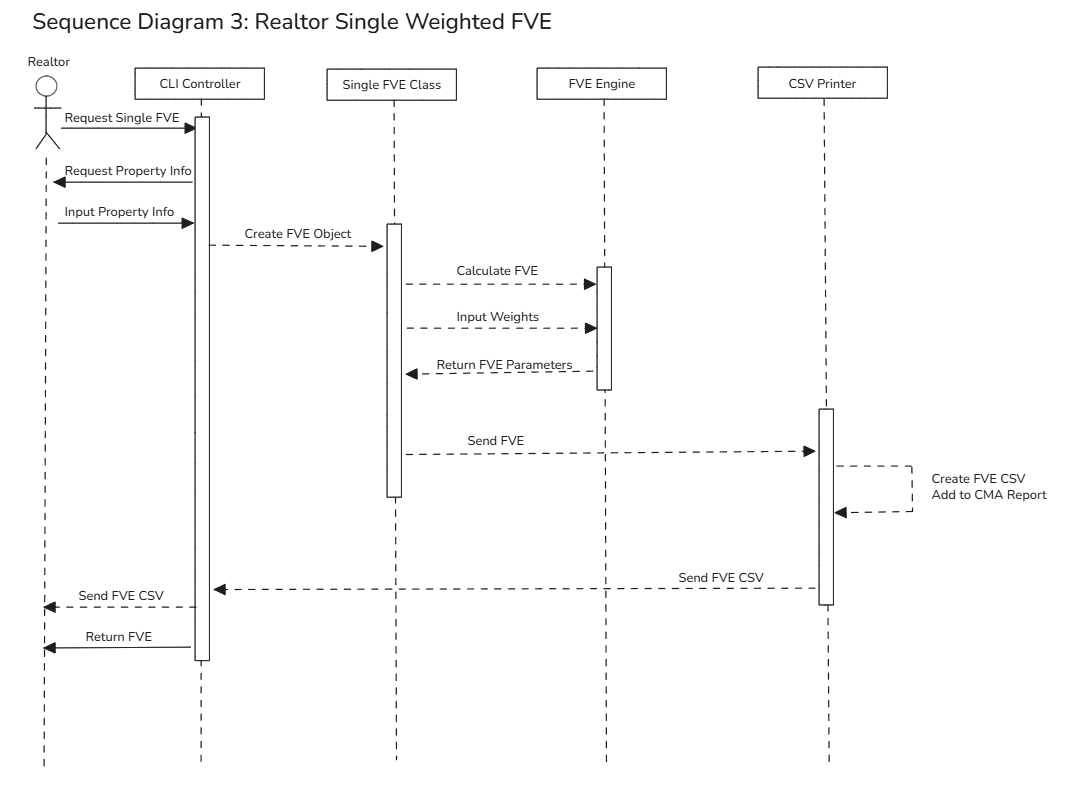
\includegraphics[width=5.69456in,height=4.19792in]{./media/3e07a12ca4d6746d0df9853b8ee7afc34e4cc124.png}

\emph{Here is a single weighted FVE. The only difference from the
unweighted single FVE is that the FVE class now sends the input weights
to the engine. Everything else remains the same.}

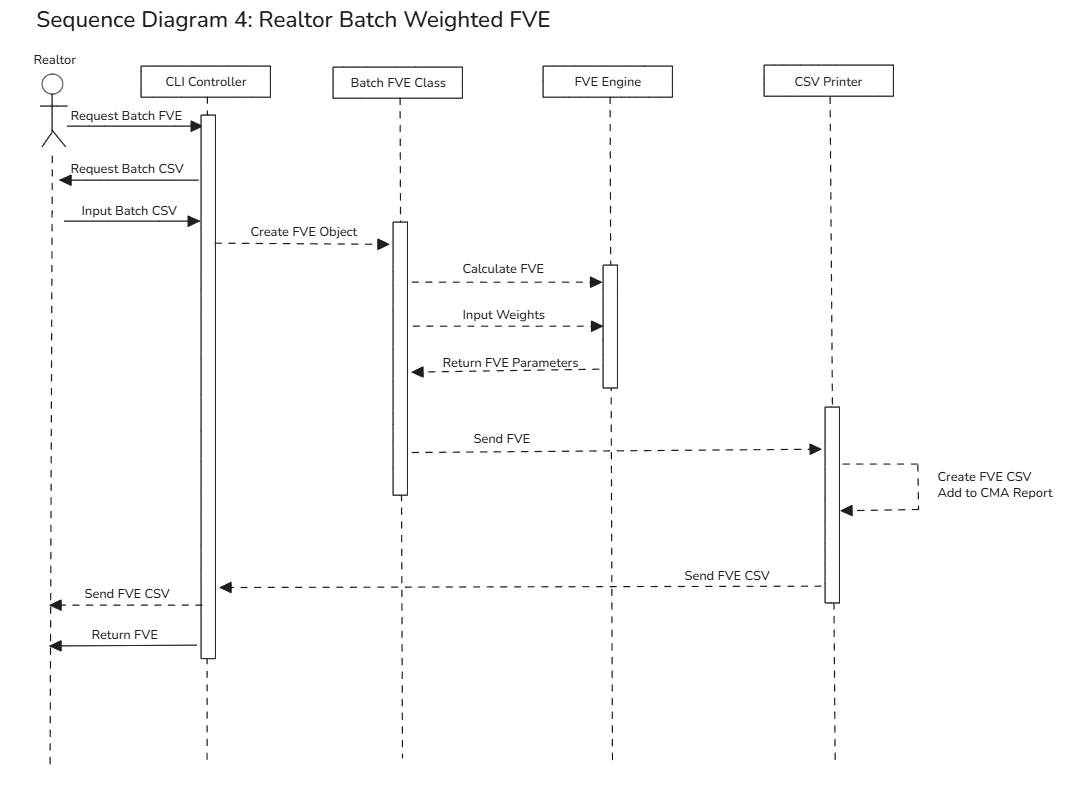
\includegraphics[width=5.8393in,height=4.27654in]{./media/66a1d75379b51ebe29d7846c200868445d4b4c37.png}

\emph{Here is the batch weighted FVE. It works the same as the
unweighted batch FVE, with the exception that the batch FVE class now
sends the client's weights.}

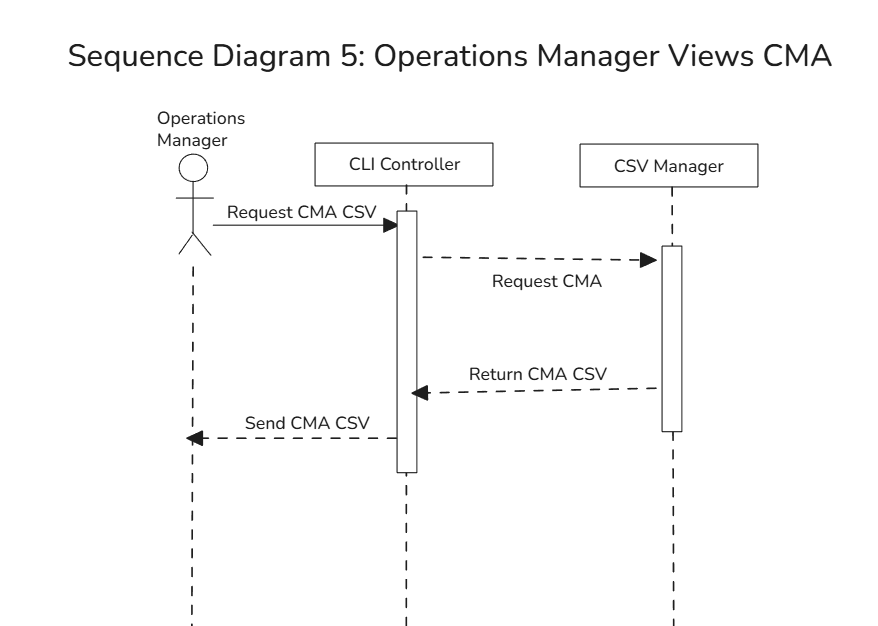
\includegraphics[width=5.85872in,height=4.17809in]{./media/f7e0880d626d7abbde5cd3eb64784b0611176f8e.png}

\emph{Here is the operations manger viewing the CMA sequence diagram.
The operations manager clicks on the view CMA button, which sends a
request to the CSV manager. This then returns the directory where the
CMA is located to the user.}

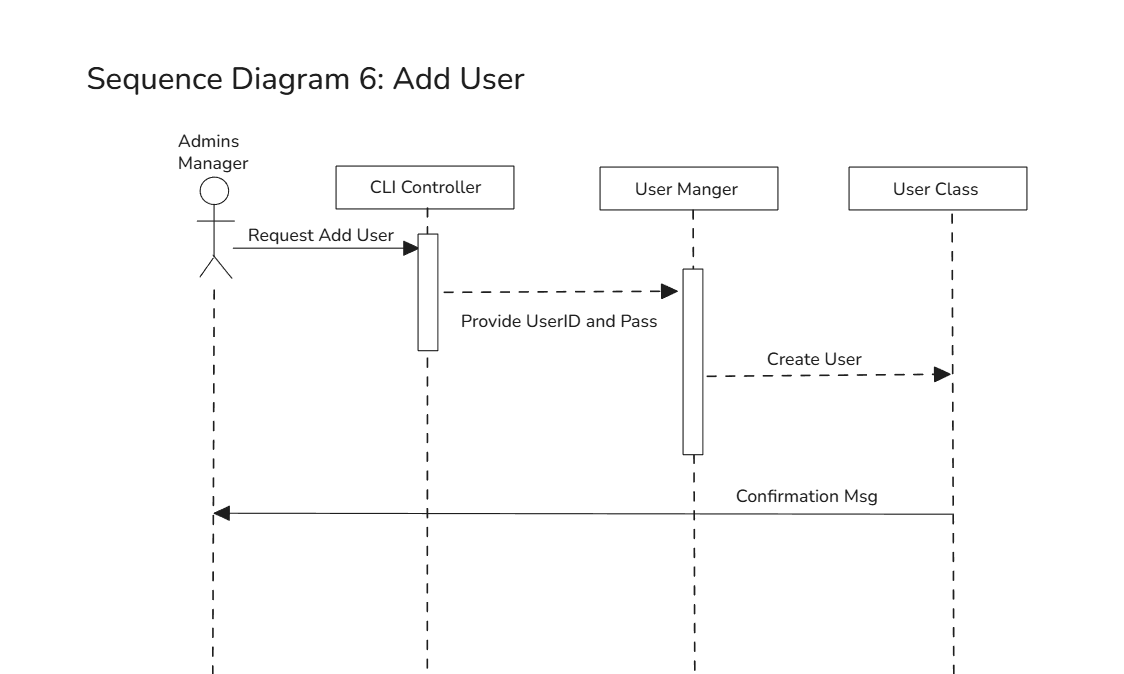
\includegraphics[width=5.84743in,height=3.50471in]{./media/09339b5c1c6708b7ce93d1c437f6d0a71347e3bb.png}

\emph{Here is a sequence diagram of the manager adding a new user. The
manager provides the new username and password, which is then sent to
the user manager. This then updates the user class, and a confirmation
message is sent to the manager.}

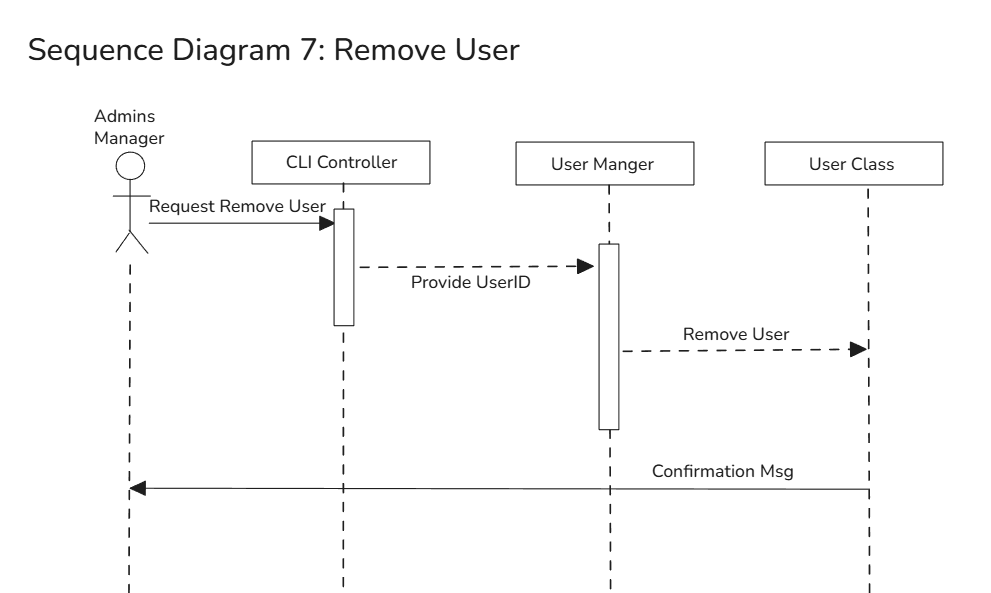
\includegraphics[width=5.80315in,height=3.46887in]{./media/a540928bff313f8636d1d92a30e50670dc8cdd08.png}

\emph{Here is a sequence diagram of the manager removing a user. The
admin provides the userID to the user manager class, which updates the
user class. A confirmation message is then sent to the manager.}

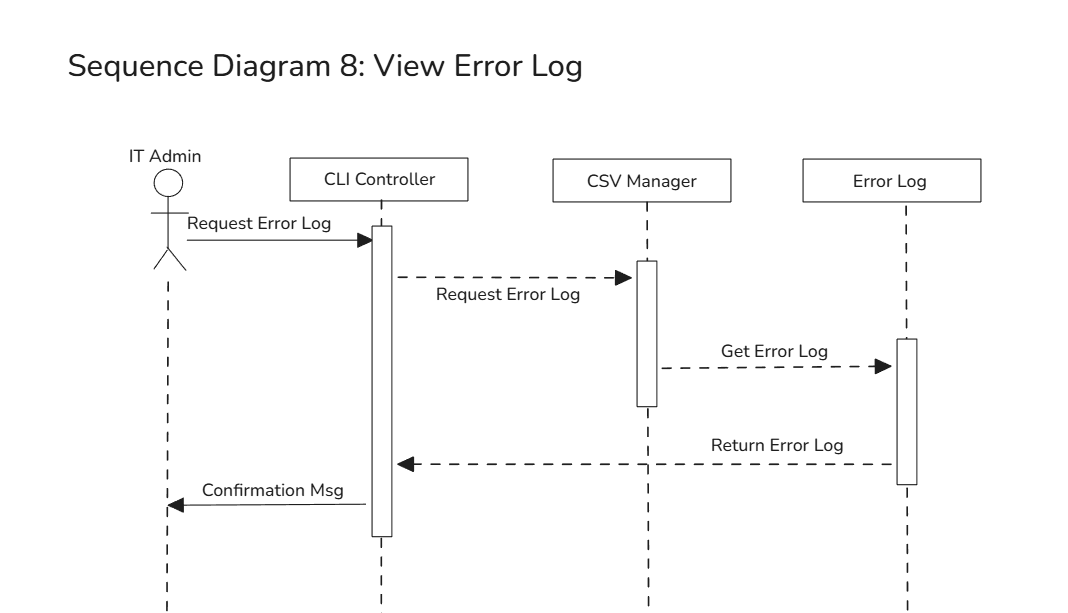
\includegraphics[width=5.92708in,height=3.40047in]{./media/50e16d342a02fa9fa9a4e6629bc679dc0ad4f4c5.png}

\emph{This is a sequence diagram of the IT admin viewing error logs for
the whole system. When the IT admin requests the error logs, this
request is sent to the CSV manager. The error logs is returned to the
CLI controller for the IT admin to view, and a confirmation message is
sent to the IT admin.}

\phantomsection \phantomsection\subsection{10.2 Class Diagrams}\label{class-diagrams}

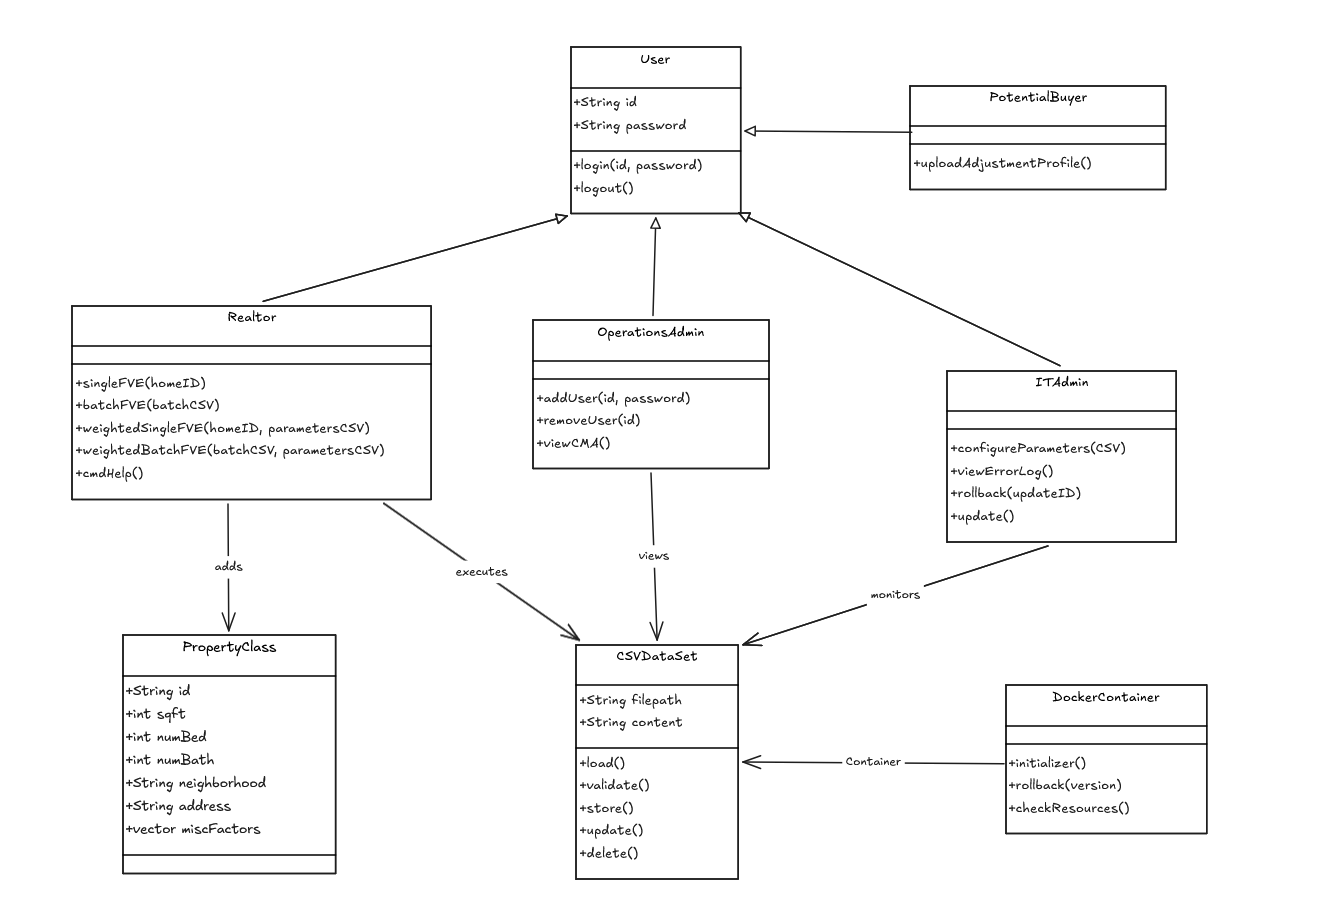
\includegraphics[width=6.5in,height=4.54167in]{./media/db9b38eb794215dc8c5d0ab1970118d515c5573b.png}

\emph{Here is a class diagram for the entire system. It shows the user
class and all of its subclasses, being the realtor, operations manager,
the IT admin, and the potential buyer. It also shows three other
classes; being the property class, the CSV dataset, and the Docker
container. The realtor adds the property class and executes the CSV
dataset, the operations manager views the CSV dataset, the IT admin
monitors the CSV dataset, and the Docker container containerizes the CSV
dataset.}

\phantomsection \phantomsection\subsection{10.3 Swimlane Diagrams}\label{swimlane-diagrams}

\includegraphics[width=6.5in,height=4.98958in]{./media/f70a791cc2945f679b07348cfb5b9656f501b04f.png}

\emph{This is a swimlane diagram for the log in system. The
authentication system first checks if the credentials are valid, then
identifies the user's role before registering the user in the system.}

\includegraphics[width=5.70833in,height=6.5in]{./media/be5b971583c3e4534164f4541adb4b07d744438a.png}

\emph{Here is a swimlane for the FVE engine. After the realtor is signed
in, the realtor inputs a property dataset CSV, which is checked for
valid parameters. This is brought to the FVE engine, which parses the
parameters. An FVE is then calculated, after which the system checks if
it should be a single FVE or a batch. A batch FVE is sent to the admin
manager to review before it is given back to the FVE for the final
report. A single FVE is sent straight to the final report.}

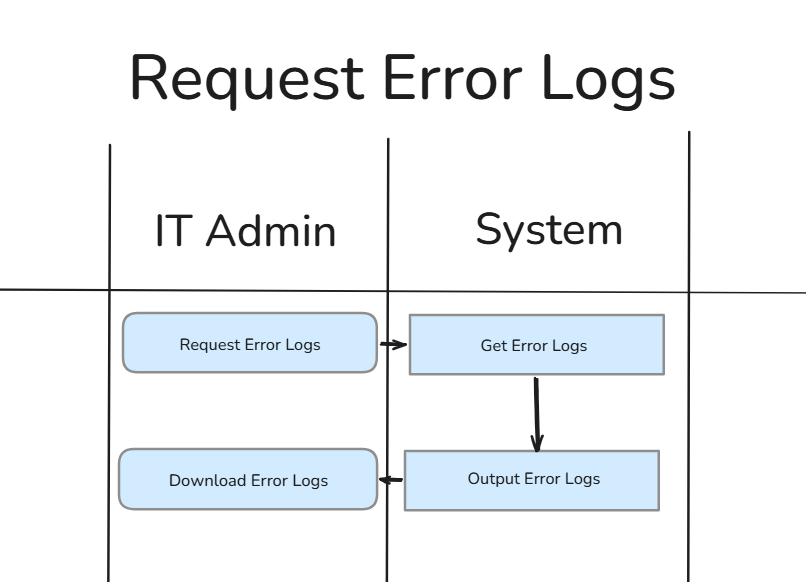
\includegraphics[width=5.08333in,height=3.67401in]{./media/46e9e9babc6ccefd1ca704c50cbe3095cd58fd10.png}

\emph{The error logs swimlane is fairly simple. The IT admin requests
the error logs, and the system returns a CSV of the error logs.}

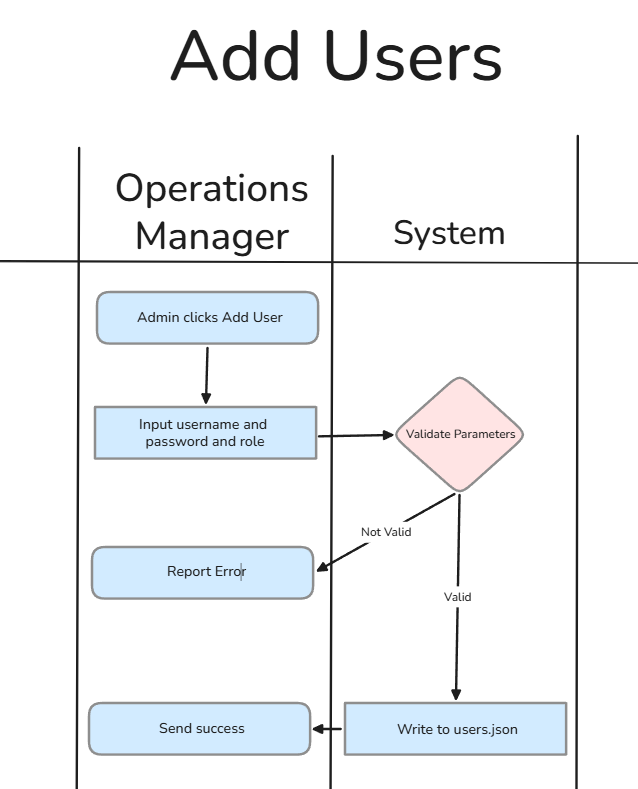
\includegraphics[width=5.1171in,height=6.32292in]{./media/bb048f990b91c14822b6f61785c2b6746a5312cd.png}

\emph{For the add users swimlane, the operations manager first inputs
the username, password, and role of the user to be added. The system
verifies that the parameters are correct, then writes to the users.json
file the new user.}

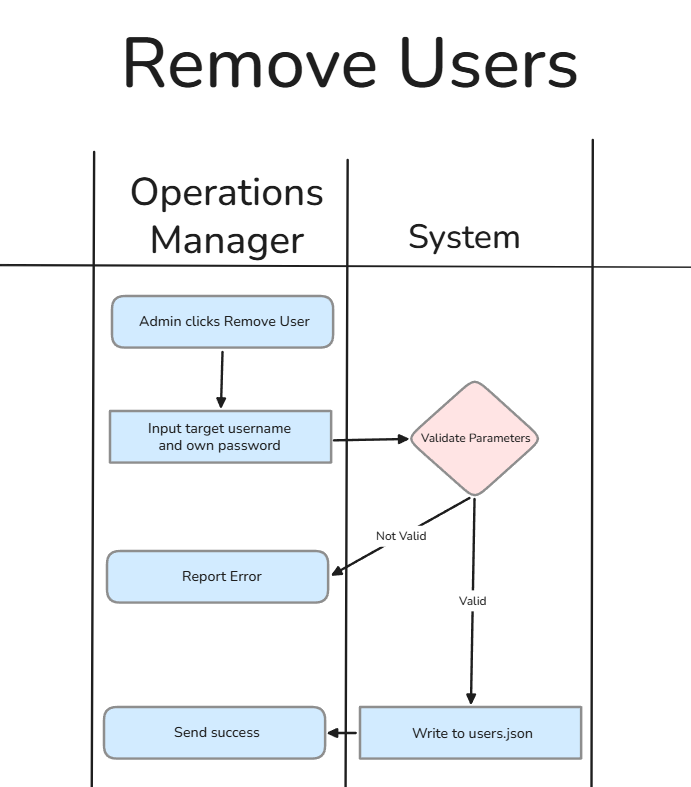
\includegraphics[width=5.70833in,height=6.5in]{./media/ce48e1b70c1ede91a7a129c0c7409e2b24a37262.png}

\emph{For the remove users swimlane, the operations manager first inputs
the username of the user to be added and their own password. The system
verifies that the parameters are correct, then writes to the users.json
file to remove the target user.}

\phantomsection \phantomsection\section{11. Software Implementation}\label{software-implementation}

\phantomsection \phantomsection\subsection{11.1 Architectural Overview}\label{architectural-overview}

The application utilizes a modular, layered logical architecture
centered around a Node.js runtime and Ink-based CLI UI composition. The
system implements a secure Authentication layer and Role-Based Access
Control (RBAC) which gates access to functional modules. These UI
components interface with a decoupled service layer which contains the
calculation matrix, user management, and authentication services. The
entire system is then mounted on a File-based Persistence Layer using
CSV and JSON formats. This containerized solution is deployed via Docker
on a mesh network using ttyd (Web-Based Terminal), allowing authorized
users to access the CLI interface directly through their web browser.

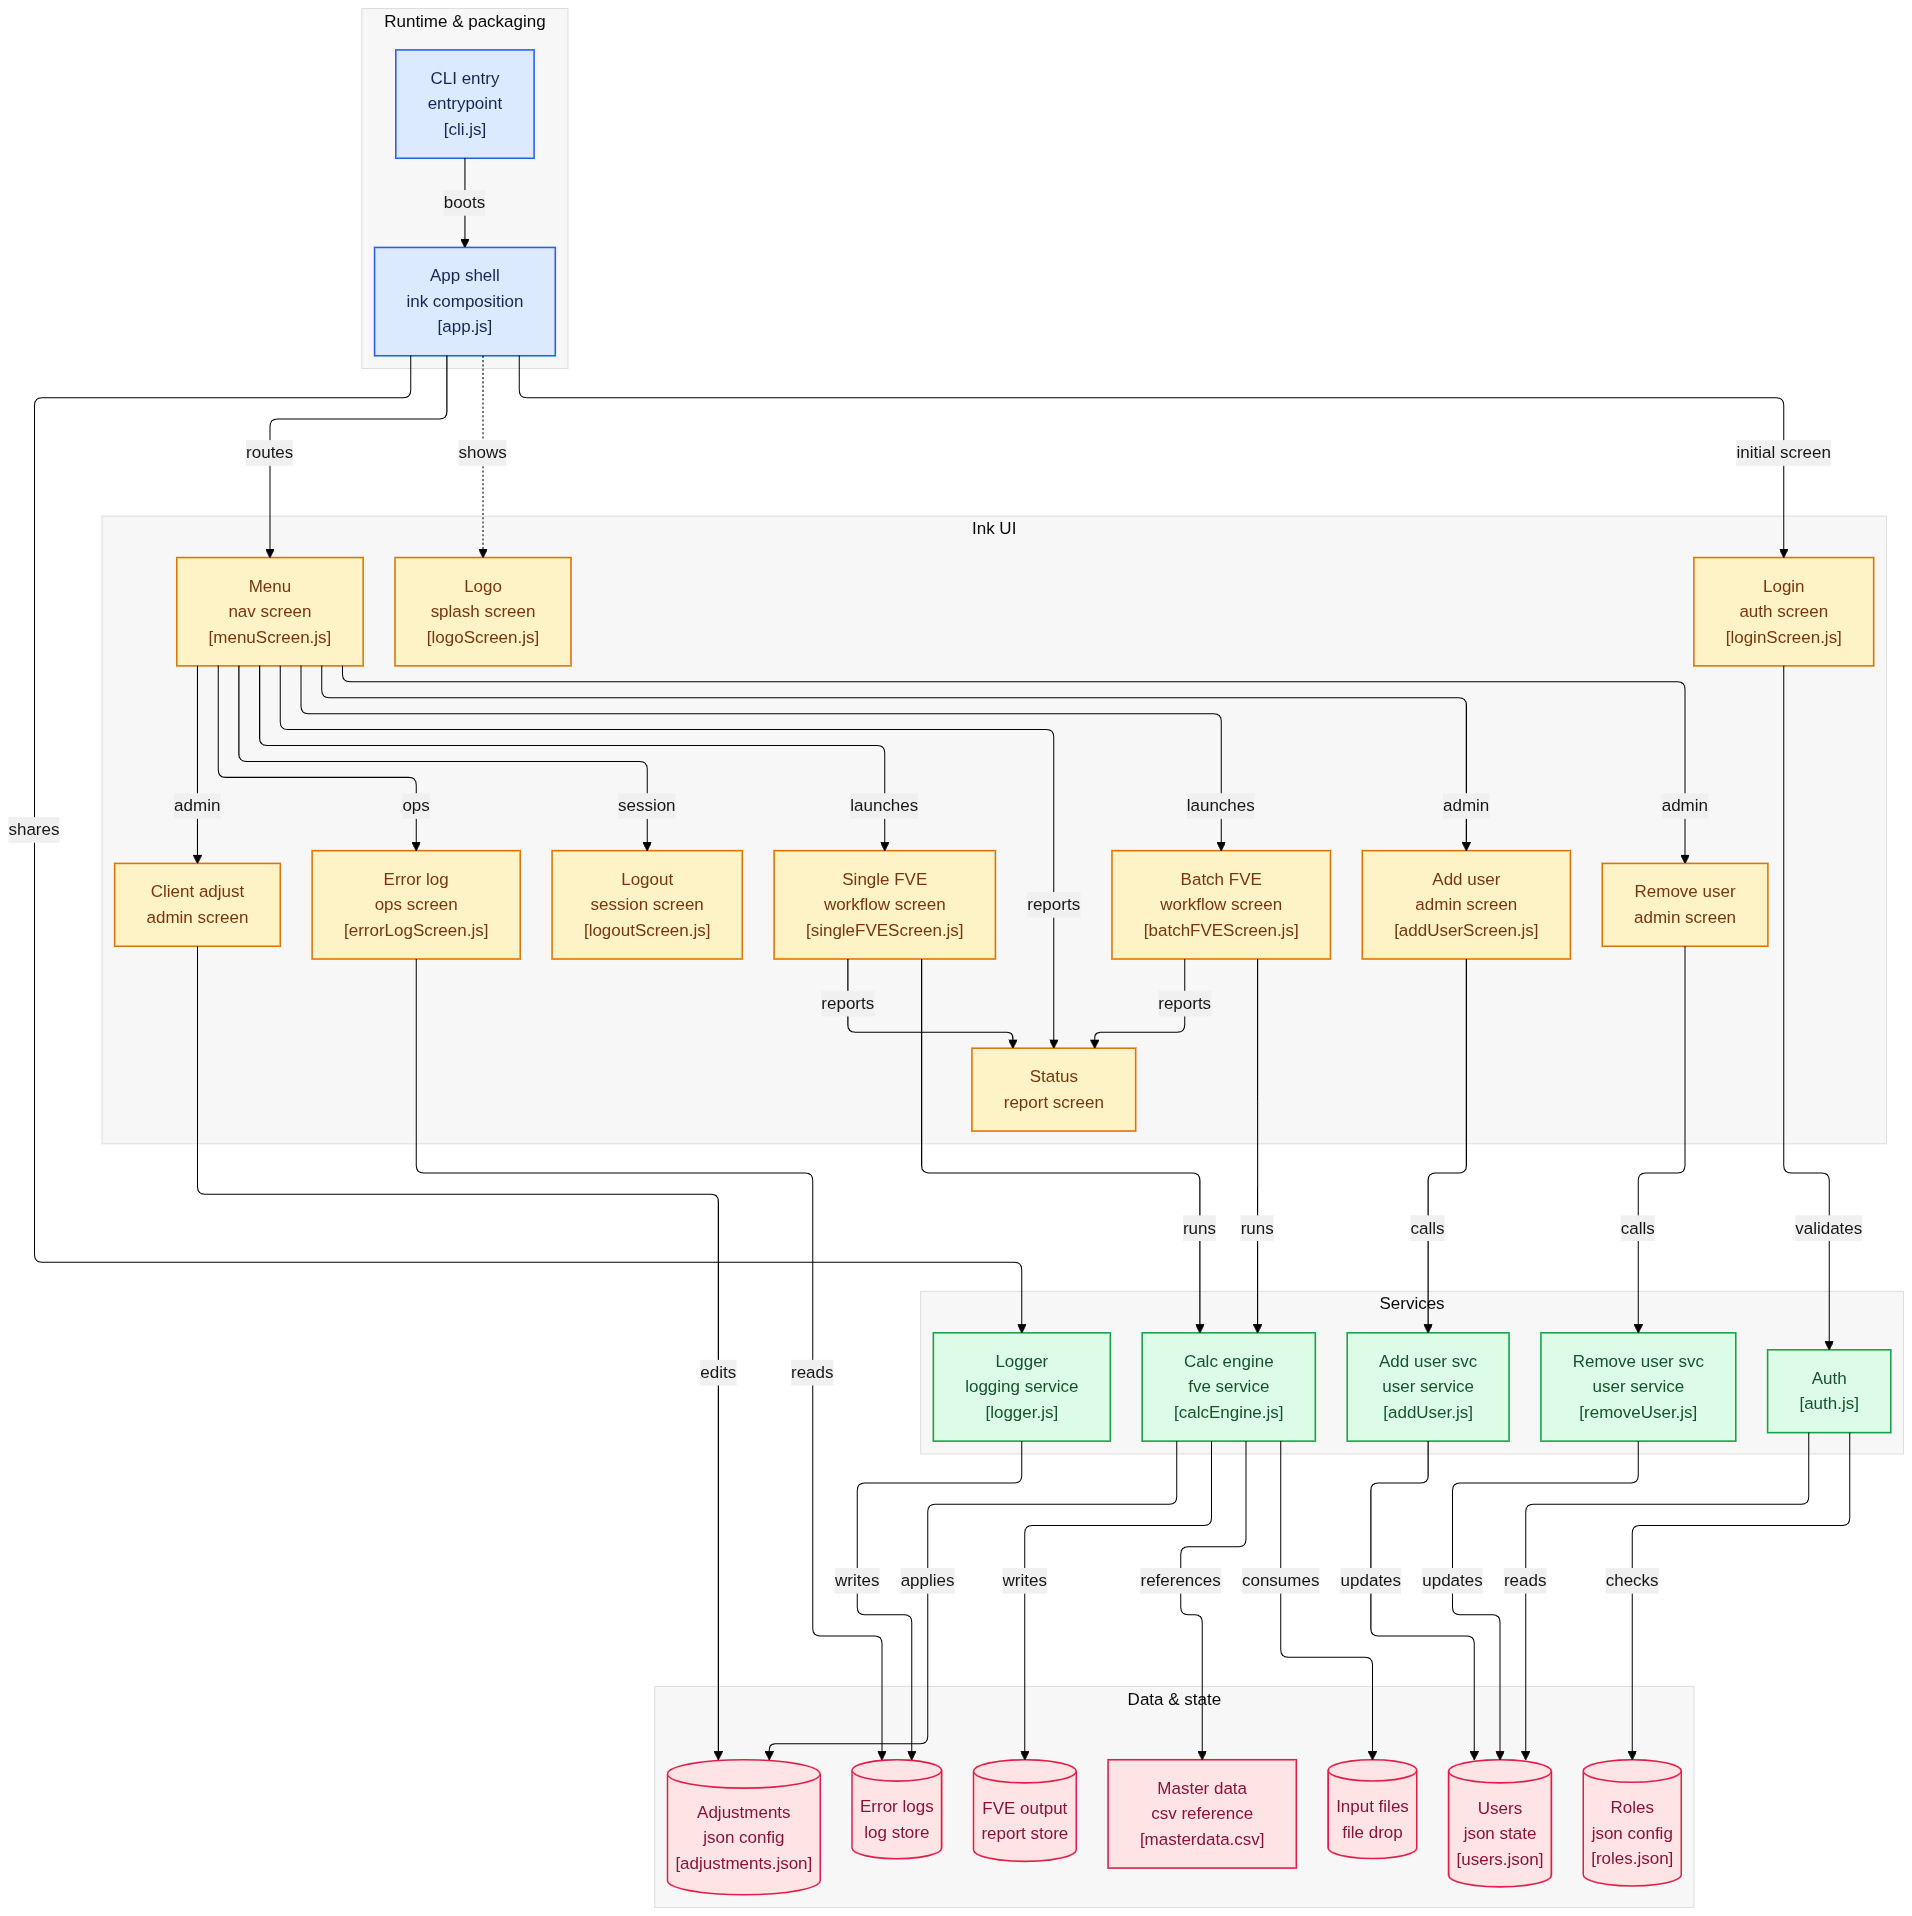
\includegraphics[width=5.90246in,height=5.91194in]{./media/aab6443cf0148f7007814a638674416d1abbc0af.png}

\phantomsection \phantomsection\subsection{11.2 Role-Based Access Control \&
Authentication}\label{role-based-access-control-authentication}

The application implements a robust RBAC framework to enforce security
and ensure that system functions are aligned with specific business
orientations. Access is partitioned into four primary user classes: IT
Admin, Operational Manager, Realtor Agent, and Business Analyst. These
roles are defined within a centralized `roles.json` configuration file.
User credentials are maintained within the persistence layer which the
system queries during the login process for verification and
authentication.

Upon successful session login, the application dynamically renders the
main navigation menu which grants core functions based on the assigned
role configuration.


\includegraphics[width=3.17086in,height=2.55159in]{./media/d7c610f422d34c6c8e41ef79cd9f77bd6b137ddd.png}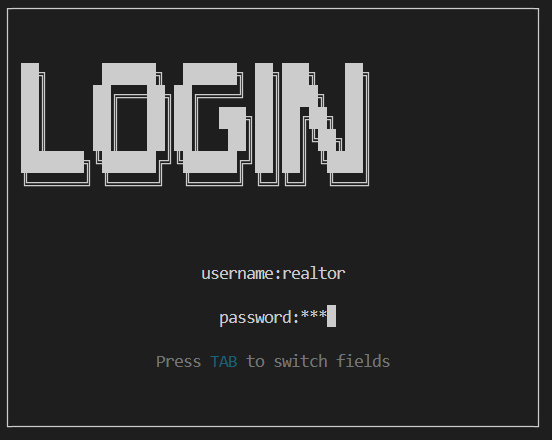
\includegraphics[width=3.19838in,height=2.54943in]{./media/7179060cb512758e77cd4db3f8f9ad8ae4ff5bab.png}

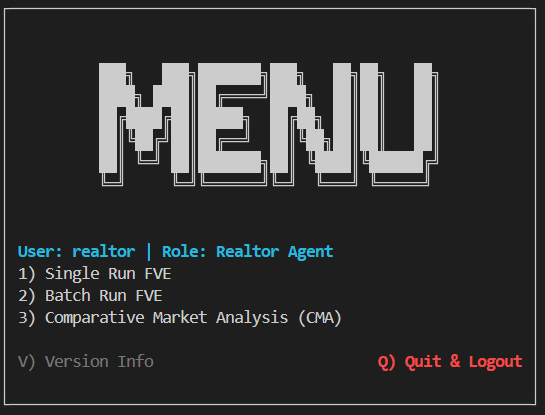
\includegraphics[width=3.30399in,height=2.51588in]{./media/7ec10809bb650c00b7530cde2136fcbfeda1ce26.png}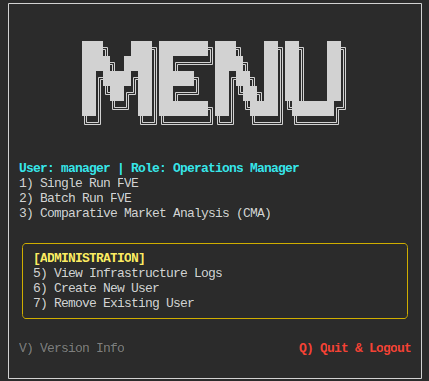
\includegraphics[width=2.74519in,height=2.43804in]{./media/fbcb9fc398549a300d9c28bc4d37e1f7df6481ab.png}

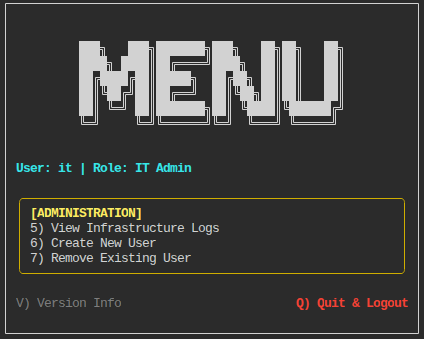
\includegraphics[width=2.78836in,height=2.22938in]{./media/e317b72cbfb412908b379032d935ba2dcbc3f695.png}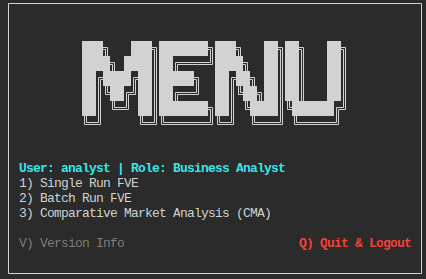
\includegraphics[width=3.52716in,height=2.31004in]{./media/856d85cbc3ccf903062ed81a41eead661bcda9e1.png}

\phantomsection \phantomsection\subsection{11.3 Fair Value Estimator
Engine}\label{fair-value-estimator-engine}

User classes like Real Estate Agents, Business Analysts, and Operational
Managers are granted access to the FVE engine to get a FVE report on
either a single property or a batch of properties. This module automates
property valuations through a structure pipeline of data ingestions,
geospatial analysis, and comparative market analysis modelling. By
evaluating similar properties against the subject ``evaluatee'', the
calculation engine generates THREE (3) critical datapoints: a Fair Value
Estimate of the property in dollars, a count of similar listings
identified and used in the generation of the FVE, and a confidence
rating regarding the accuracy of the FVE.

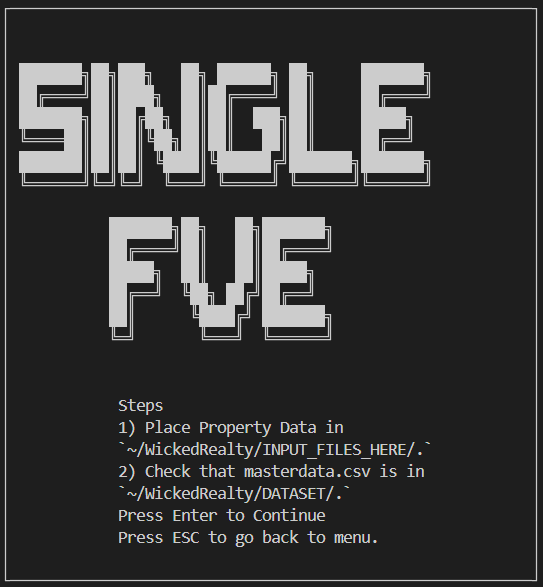
\includegraphics[width=2.03413in,height=2.19895in]{./media/673be7b41a78dd5f7a9eeb906683cc9c9cea95e8.png}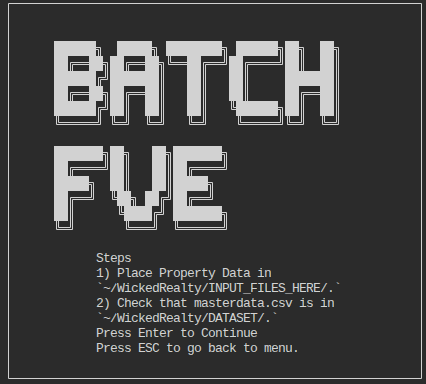
\includegraphics[width=2.3186in,height=2.09in]{./media/182af4efd5989d321e3619acf2ab3976861f0b93.png}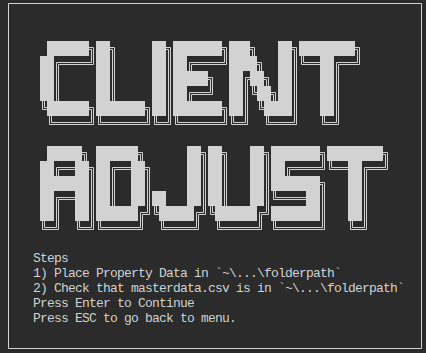
\includegraphics[width=2.41162in,height=1.99836in]{./media/31f848e93a581c46c62a339e110799cf6e1559a5.png}

Users are also provided with immediate visual feedback via a dedicated
Status Screen where successful runs are highlighted in green with
finalized reports automatically exported to the
`\textasciitilde/WickedRealty/FVE\_OUTPUT` folder while failed runs are
rendered in bold red with specific diagnostic error messaging.

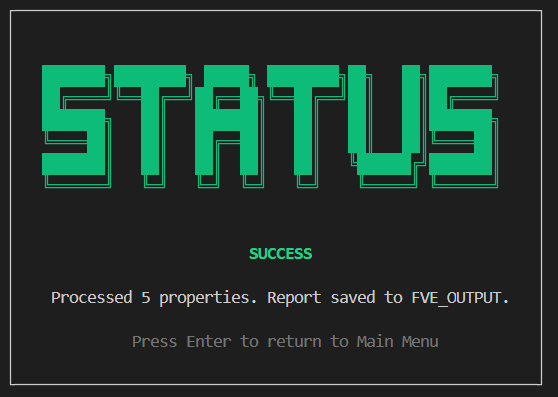
\includegraphics[width=3.3385in,height=2.37524in]{./media/fcbd5341d016cc3272be331455ba65810af7acd5.png}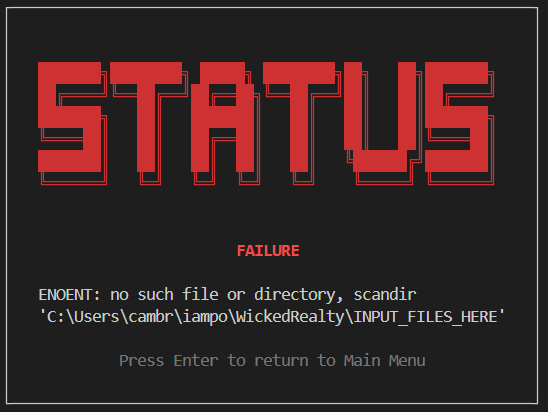
\includegraphics[width=3.12483in,height=2.34932in]{./media/a81f8947028d1d1eaca2f6950dd52ab2c127b1c9.png}

The current system has been stress tested with a dataset of 20,000
listings, and it was able to generate the single FVE in under 0.2
seconds, well under the 5 second success metric that was agreed upon by
the client.

\phantomsection \phantomsection\subsection{11.4 System Management}\label{system-management}

The System Management module provides privileged users like IT Admin and
Operational Managers with the tools necessary to maintain the
application's integrity and manage user lifecycles. These administrative
functions ensure that access remains secure, and that system health is
monitored in real-time with ease.

This module allows authorized users to create new accounts in the system
with a unique username, secure password, and user class. Conversely, the
module also grants the authority to remove existing users.

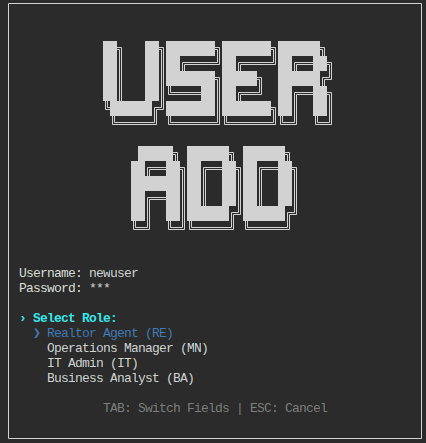
\includegraphics[width=2.97717in,height=3.09598in]{./media/2a1e5a7ab4ed68bb7b0b169e87ccf3309f5f9613.png}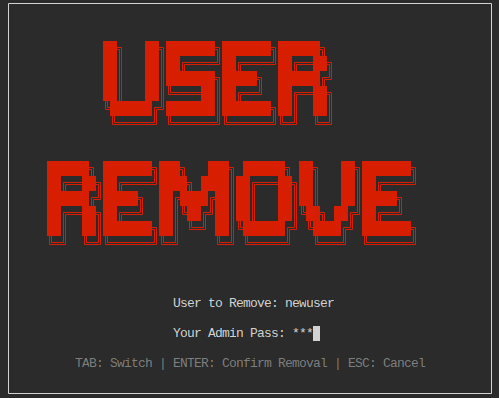
\includegraphics[width=3.35906in,height=2.67917in]{./media/b243d3bcfd192cfbd77cedcdce5b31992baf0048.png}

Roles with access to this module are also granted exclusive access to
the Infrastructure Error Logs which aggregate recent system faults and
error traces, divided by day. This provides detailed information which
will allow system administrators to identify system anomalies and
maintain the system throughout its lifecycle.

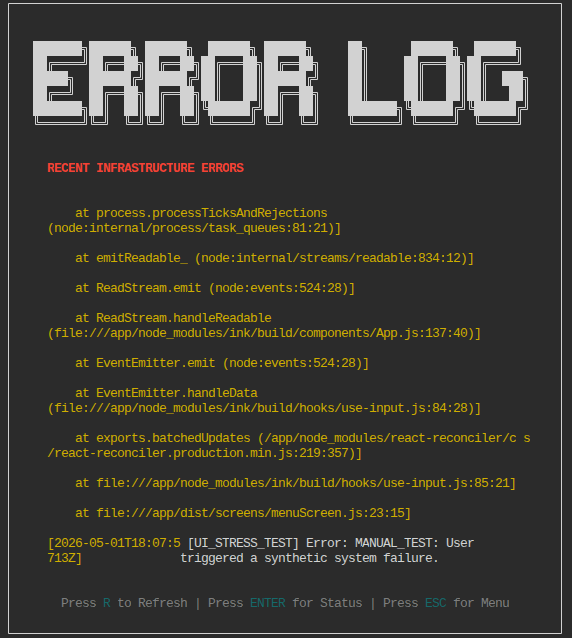
\includegraphics[width=3.63442in,height=4.05703in]{./media/ca50de1d38a0629e939ad9e1f5bf36c7a2e92cde.png}

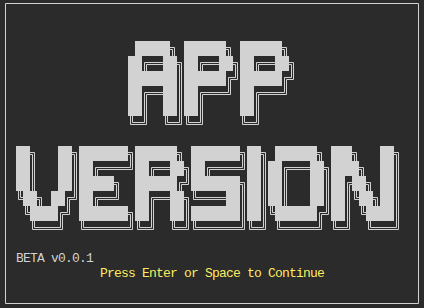
\includegraphics[width=3.12535in,height=2.2703in]{./media/10ce7d01ccc458cee1adb46b6cd87db69651efc6.png}

The application was containerized in Docker and deployed on a mesh
network which allows authorized users to freely connect via the assigned
port from the convenience of their web browser.

\phantomsection \phantomsection\section{12. AI Usage Reflection}\label{ai-usage-reflection}

\phantomsection \phantomsection\subsection{12.1 RD1.0 AI Usage}\label{rd1.0-ai-usage}

Our team originally tried using our preferred LLM models, e.g.
SurfSense/Gemini, to give us a few ideas about how to fill each section.
However, when attempting to prompt, we were constantly recommending an
obscene amount of microservices that we didn't exactly need given our
project was for a small-scale modern application to solve a niche need.

While we attempt to guide the LLMs toward using less
microservices/smaller infrastructure, it took much more refining and
hand holding than we wanted to do. Hence, we ended up writing all the
document ourselves given: a) we're implementing this product, so knowing
what is being put down is more useful than having it generated, b) any
issues/questions are more quickly addressed during this planning phase,
c) each group member knows their part more clearly and roles are easier
to distribute.

Examples of us guiding the LLMs included using words such as
``hypothetically'', ``no microservices'', ``small scale'' and directly
feeding resources that we desired it to emulate (such as the proposal
document). While it generated \emph{ok} answers, there was a lot left to
be desired.

The main software aid we used in writing was a spellcheck which MS word
provided by default. However, given this isn\textquotesingle t
generative (as there isn't exactly any prompting or tokens being used),
we don't really have much else to provide for this section. Grammarly
was used for some sections, but again, was used for the spell-checking
features, not for any generative usages (again no prompts or anything
used here).

\phantomsection \phantomsection\subsection{12.2 RD2.0 AI Usage}\label{rd2.0-ai-usage}

Multiple AI aids were used in the creation of RD2.0. To start, ChatGPT
was used to generate the equations in the revisions in section 2.d. The
equations were then edited to better fit the requirements. The
conversation can be seen here
\url{https://chatgpt.com/share/69d31ef6-5648-832e-b6f5-f501e3099fd5}.

The next use of AI was Gemini 3.1. We were unsure how backwards
traceability and forwards traceability should look in section 5, so we
generated templates for both using Gemini 3.1. This saved time as we
were able to get a sense of direction on what each section should look
like, which lets us fill in with our own information. Section 5.2-5.3
used ChatGPT to help Jax look through our overall document and find the
correct links for forward and backwards traceability. Section 5.6 was
explored with ChatGPT as there were multiple ways to store the output,
and we wanted to view all our options. Ultimately, we decided to output
a CSV. The conversation can be seen here
\href{https://chatgpt.com/share/69d322f8-0c18-8325-9ded-d7c6a718542b}{https://chatgpt.com/share/69d322f8-0c18-8325-9ded-d7c6a718542b.}

\url{https://chatgpt.com/share/69d32b34-5088-8329-be16-b2c571a83460}

On section 6.1, Gemini 3.1 was used to suggest ideas on what UI external
interface requirements were useful. AI suggested a color differentiated
text coloring to improve readability between successful executions,
non-fatal warnings and critical errors. This can be further explained
below.

Section 7 uses Claude to revise some requirements for reliability,
availability, and scalability. For better context, an imported R.D. 1.0
was added to get a foundation of our project goals and ideas. Added to
the prompt was the feedback that the TA has given us members, ensuring
that it gives us better detailed output for what necessary steps for
each requirement. Claude AI suggested adding various requirements that
resigned with the project to reliability, availability, and its
scalability. We also provided constructive feedback about our own ideas
for specific required sections and asked if that resided well with the
project, resulting in a more defined and clear explanation that is more
desirable to the detail we needed.

\url{https://claude.ai/share/38507f24-ae9f-4378-b34e-503cf4bf5366}

Section 8 used Gemini 3.1 to help find directions in the slides for each
diagram type mentioned. Gemini was then asked to help decide on an
architecture type, eventually landing on a layered approach and to
provide a picture, which was discarded. From there, further questions
were asked to clarify directions for some diagrams, like the use-case
diagram. This discussion can be found here
\url{https://gemini.google.com/share/842fdc286a0a}.

Ephraim\\
\ul{Section 5-4}
Gemini 3.1 Prompt: Give me examples on how forward traceability can be
integrated into section 5-4 of the document.

Response: ``\textbf{Verification:} User Acceptance Testing (UAT) where
agents or system analysts trigger the CMA report generation for a target
property via the platform interface. Testers will download the resulting
CSV file and open it in a standard spreadsheet application (e.g., Excel
or Google Sheets) to verify that the file structure is intact (no broken
columns), and that the computed FVE, geospatial parameters, and list of
comparative properties are accurately mapped to their respective
columns. Automated integration tests will also verify that the CSV file
is generated within the expected time limit and correctly saved to the
designated file directory.''\\
\strut \\
How it was used: Section 5-4 adopted the User Acceptance Testing
suggestion whereby testers and agents can test as they use the system.
The automated integration tests were also adopted to verify the
functionality of the system feature.

Gemini 3.1 Prompt: Show me an example of a full user story for IT
administrator including narrative and acceptance statements.

Response: ``\textbf{Narrative:}

\begin{itemize}
\item
  \textbf{As an} IT Administrator,
\item
  \textbf{I want to} access detailed error logs whenever the FVE
  calculation or CSV generation process fails,
\item
  \textbf{so that} I can rapidly troubleshoot API timeouts, missing
  geospatial data, or file storage permission errors without relying
  solely on agent bug reports.
\end{itemize}

\textbf{Acceptance:}

\begin{itemize}
\item
  \textbf{Given} the FVE engine encounters a system error (e.g., a File
  Write/Permission Failure during CSV export),
\item
  \textbf{When} the system halts the process and returns an error to the
  user,
\item
  \textbf{Then} the system writes a standardized log entry to the
  administrative console containing the timestamp, specific error code,
  and the property ID that triggered the failure.
\end{itemize}

''\\
How it was used: This template gave us a good idea over how to structure
the user stories section and was helpful in understanding how an
acceptance statement was written. We adopted this template for Section
5.\\
\strut \\
\ul{Section 6.1}
Gemini 3.1 Prompt: Give me examples what are some user interface
requirements that should included.

Response: ``

\textbf{a. User Interfaces} This section describes the boundary between
the human user and the system. Given the constraints of the project, the
primary interface is strictly text-based and accessed via a standard
terminal emulator (e.g., Windows Command Prompt, PowerShell, macOS
Terminal, or Linux bash/zsh).

\begin{itemize}
\item
  \textbf{Format \& Style:} * The interface shall be a Command Line
  Interface (CLI) designed for minimalism, speed, and low resource
  overhead.

  \begin{itemize}
  \item
    The system shall utilize standard output (stdout) for successful
    executions and standard error (stderr) for failure states.
  \item
    To improve readability for non-technical real estate agents, the CLI
    shall implement basic text coloring (e.g., Red for
    errors/exceptions, Green for successful valuations/exports, and
    Yellow for warnings like missing optional data).
  \end{itemize}
\item
  \textbf{Interaction Constraints:}

  \begin{itemize}
  \item
    \textbf{Command Execution:} Users will interact with the system
    using standard POSIX-style command syntax consisting of a base
    command, an action, and specific flags/arguments.

    \begin{itemize}
    \item
      \emph{Example Syntax:} fve-engine calculate-solo -\/-file
      \textless property\_filename.csv\textgreater{}
    \item
      \emph{Example Syntax:} fve-engine calculate-batch -\/-dir
      \textless directory\_path\textgreater{} -\/-radius 5
    \end{itemize}
  \item
    \textbf{ASCII Menu Navigation:} For users uncomfortable with raw
    command syntax, executing the base command (e.g., fve-engine)
    without arguments will trigger an interactive ASCII-formatted text
    menu. This menu will allow users to select operations (e.g., "1. Run
    Single FVE", "2. Run Batch CMA") using numeric key presses.
  \item
    \textbf{Feedback Mechanisms:} For batch processing (up to 100
    properties), the interface shall display an ASCII progress bar or
    percentage indicator to provide the user with real-time feedback on
    system execution.
  \item
    \textbf{Help Dialogues:} Appending -\/-help to any command will
    output a formatted table of valid syntax, required arguments, and
    usage examples directly into the terminal window.
  \end{itemize}
\end{itemize}

How it was used: I really liked how basic requirements like color coded
texts could make a really large impact in terms of bridging the gulf of
execution and evaluation. We adopted the idea that the CLI would STDOUT
green for successes, yellow for warning, and red for stopping failures.
This is often overlooked and not part of most CLI applications, which I
personally find wanting.

\phantomsection \phantomsection\subsection{12.3 Arika's AI Usage Stack}\label{arikas-ai-usage-stack}

Section 6.2 onwards was all written by hand with NO AI involved.
Additionally, much of Section 7 was overhauled by hand as a lot of
written prompts did not make any sense. They were written to confirm
with the docker standards outlined as written by hand in section 6.2
onwards. Many sections were modified in order to cleanly flow from
section to next section. This was done by hand without AI.

The overall knitted document used a variety of AI agents to double-check
the entire document. The workflow is as follows:

DISCLAIMER: As with all AI tools, I understand that they are good for
generating templates not for actual code. Overly relying on AI generated
code quickly leads to immense tech debt and what many people call "vibe
coding clean-up" roles. Most of what was used was either a) proof of
concept to see how well the tools fair with heavy user influence, or b)
to check existing work currently written as a "helper" to optimize
performance and readability.

While documentation was tidied and used to generate suggestions with the
Gemni CLI workflow, most of it still ended up handwritten.

The primary use of AI used two main tech stacks:

\begin{itemize}
\item
  surf sense (\url{https://www.surfsense.com/})
\item
  gemni cli (\url{https://github.com/google-gemini/gemini-cli})
\end{itemize}

GSD (getshitdone) was used for the initial project planning (as seen
below). Then I manually went in and edited by hand parts that
didn\textquotesingle t seem good, or fit with the code structure.

Gemni CLI

I used the following GSD model ontop of gemni CLI to better verify the
work and assumptions done:

\begin{itemize}
\item
  getshitdone (\url{https://github.com/rokicool/gsd-opencode})
\end{itemize}

Additionally, I have my own custom rule-set script which is pretty long
so won\textquotesingle t be included here.

Several model types were used dependent on what needed to be done.

As with most GSD workflows for each new PDN project I would go with the
following:

\begin{itemize}
\item
  Initialization (/gsd-new-project)
\end{itemize}

- Initial questions

- PDF Document upload of problems

- Assumptions being made (and fixed)

- Code style wished to be generated

- codebase linked

- README generated

- Point towards internal data that should be used (all 3 textbooks, path
to local repo)

\begin{itemize}
\item
  Research
\end{itemize}

- Custom phase with gemni

- able to do more in depth analysis of the project given along with
sources pointed to

- additionally looks out for more sources online

- I usually search myself for stackoverflow topics I may think useful. I
will then point it to my surfsense model to see if it makes sense to
implement it, then feed it to GSD to write

in.

\begin{itemize}
\item
  Planning (/gsd-plan-phase )
\end{itemize}

- Split each problem and sub problem into their own atomic phases/tasks

- A plan checker ensuring nothing was missed

- Context Isolation and verification of tasks

\begin{itemize}
\item
  Execution (/gsd-run-phase )
\end{itemize}

- execution of per phase as outlined in generated README

- tasks are run per wave with atomic commits

- Each commit is then showed of what changed and I can go in and ask /
edit the changes it made

\begin{itemize}
\item
  Verification
\end{itemize}

- Spawn any debug agents

- generate potential ticket issues

How Agents Work in Gemini CLI

In the Gemini CLI and GSD workflow, "agents" are specialized AI
instances that can be spawned to handle specific, focused tasks. Think
of them as delegating a piece of your project to an

expert who specializes in that one area. This is a core concept for
efficiently managing complex software projects.

Key Concepts:

\begin{itemize}
\item
  Delegation: Instead of having one single AI context trying to manage
  everything from high-level planning to low-level code fixes, you
  delegate. For example, when you run
\end{itemize}

/gsd:plan-phase, you are spawning a gsd-planner agent whose sole job is
to create a high-quality, executable plan.

\begin{itemize}
\item
  Specialization: Each agent is optimized for its role.

  \begin{itemize}
  \item
    gsd\_phase\_researcher: Scours the web and provided documents for
    information.
  \item
    gsd-planner: Breaks down goals into concrete, verifiable steps.
  \item
    gsd\_codebase\_mapper: Analyzes existing code to understand its
    structure and conventions.
  \item
    gsd\_verifier: Checks if the completed work actually meets the
    original goals.
  \item
    generalist: A flexible agent that can be given a wide range of
    tasks, often used for batch operations or speculative investigations
    without cluttering the main chat.
  \end{itemize}
\item
  Parallelism \& Isolation: Agents can often work in parallel. You could
  have one agent researching an API while another maps out the existing
  codebase, speeding up the overall process.
\end{itemize}

Their work is also isolated, preventing them from interfering with each
other.

\begin{itemize}
\item
  Workflow Orchestration: The main GSD process orchestrates these
  agents. It spawns them as needed, feeds them the necessary context,
  and integrates their results back into the main
\end{itemize}

project plan or codebase. For instance, the output of the
gsd-phase-researcher (a RESEARCH.md file) becomes the input for the
gsd-planner.

By breaking down a large, ambiguous goal into a series of smaller,
well-defined tasks handled by specialized agents, the GSD framework
provides structure, reduces errors, and ensures all

aspects of the initial request are met. You, the user, can oversee this
process, verifying the output of each agent at each stage.

Surf Sense

On top of the current sourcing, surf sense was used more as a
generalized explainer rather than giving answers for robust problems.
Surf Sense was hosted on a docker container, with an

exposed port on my home server, using tailscale to connect to the
endpoint. Several connectors were used to gather information from the
following sources

\begin{itemize}
\item
  Obsidian
\item
  Unraid
\item
  outlook
\item
  google notebook
\item
  My github
\end{itemize}

These sources are then used during query and write time to generate
quick answers. Surf Sense is generally used as a search feature to find
any pre-existing sources I may have on a topic in order to help
gemni+GSD run better.

\phantomsection \phantomsection\subsection{12.4 RD 3.0 AI Usage}\label{rd-3.0-ai-usage}

RD 3.0 was created with minimal AI usage. AI was only used for editing
RD 2.0 based off TA feedback and for the creation of the FVE engine
itself. Individuals who used AI and performed these tasks go into their
usage in detail below. For the creation of the engine, Gemini was given
an overview of the purpose, its architecture, and its tech stack before
any specific questions were asked. Any other section of the RD,
presentation, or application not mentioned below was made in its
entirety without AI.

Thuan's AI Usage:

For my AI Usage, I aimed to process improvements with the feedback from
the TA back on RD 2.0. Using AI, I summarized each RD file for context
to provide key areas in which parts were needed to improve
(\url{https://gemini.google.com/share/36247eaf84e7}), including
unrealistic criteria numbers and diagram formatting. For the swimlane
diagrams, no AI has been utilized, as most of the workflow was more so
generalized based on the format of which various visualized actors are
shown. The image provided below showcases a sketch draft of the swimlane
diagram in which the project was operated:\\
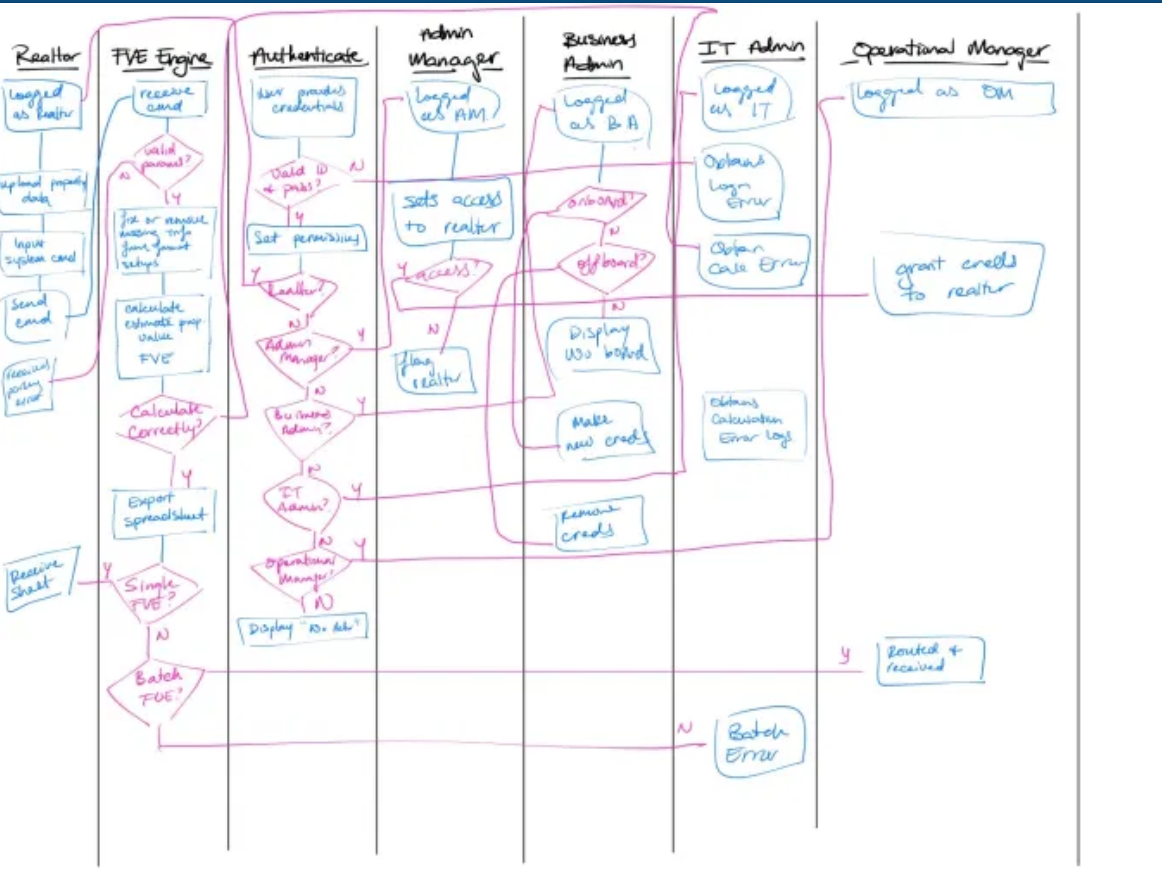
\includegraphics[width=6.5in,height=5in]{./media/74d4fc82f4d4638da77a3edd81934cd4ab5ef865.png}

Ephraim's AI Usage

Prompt: Does Ink js have a screen handler or a router similar to React
Router which can dynamically and conditionally render screens in the
application based on userState?

Gemini 3 Response:\\
Ink does not have a "built-in" screen handler or router component in its
core library. Instead, because Ink is a standard React renderer, it
relies on the React ecosystem and standard React patterns to handle
navigation.

\begin{quote}
According to the documentation and the repository structure, there are
two main ways to handle multiple screens:
\end{quote}

\hypertarget{official-recommendation-memoryrouter}{%
\phantomsection\subsubsection{\texorpdfstring{\textbf{1. Official Recommendation:
MemoryRouter}}{1. Official Recommendation: MemoryRouter}}\label{official-recommendation-memoryrouter}}

\begin{quote}
The Ink repository includes a specific \textbf{"Routing Recipe"} that
suggests using \textbf{React Router} with a MemoryRouter. Since there is
no browser history in a terminal, MemoryRouter manages the navigation
state in memory.
\end{quote}

\begin{itemize}
\item
  \textbf{How it works:} You define your routes just like a web app.
\item
  \textbf{Location in Docs:} You can find this in the recipes/ folder of
  the GitHub repo.
\end{itemize}

\begin{quote}
JavaScript

import \{MemoryRouter, Routes, Route\} from
\textquotesingle react-router-dom\textquotesingle;\\
\strut \\
const App = () =\textgreater{} (\\
\textless MemoryRouter\textgreater{}
\textless Routes\textgreater{}
\textless Route path="/" element=\{\textless LogoScreen /\textgreater\}
/\textgreater{}
\textless Route path="/login" element=\{\textless LoginScreen
/\textgreater\} /\textgreater{}
\textless/Routes\textgreater{}
\textless/MemoryRouter\textgreater{}
);
\end{quote}

\hypertarget{manual-state-management-the-standard-way}{%
\phantomsection\subsubsection{\texorpdfstring{\textbf{2. Manual State Management (The
"Standard"
Way)}}{2. Manual State Management (The "Standard" Way)}}\label{manual-state-management-the-standard-way}}

\begin{quote}
The most common pattern used by the Ink community (and often seen in
their examples) is simple conditional rendering using React useState.
This is the method we\textquotesingle ve been using in your project so
far. It is lightweight and doesn\textquotesingle t require extra
dependencies like react-router.
\end{quote}

\hypertarget{community-libraries}{%
\phantomsection\subsubsection{\texorpdfstring{\textbf{3. Community
Libraries}}{3. Community Libraries}}\label{community-libraries}}

\begin{quote}
If you want something more specialized for the terminal, there are
community-made hooks and components, though they aren\textquotesingle t
part of the core ink package:
\end{quote}

\begin{itemize}
\item
  \textbf{ink-router}: A dedicated router built specifically for Ink.
\item
  \textbf{ink-use-router}: A hook-based approach for simple navigation.
\end{itemize}

\hypertarget{summary}{%
\phantomsection\subsubsection{\texorpdfstring{\textbf{Summary}}{Summary}}\label{summary}}

\begin{quote}
If your app (Wicked Realty) is going to have 10+ screens with complex
"back" button logic, following the \textbf{React Router (MemoryRouter)}
recipe is the most robust path. If you only have a few screens (Logo
-\textgreater{} Login -\textgreater{} Menu), the \textbf{conditional
state} approach is much faster to implement and easier to debug.
\end{quote}

How it was used: I opted to use the ``standard router'' approach and
implement manual routing.

Prompt: What libraries should I consider to implement a loading spinner?

Gemini 3:

\begin{quote}
Yes, you can integrate a spinner very easily. In the Ink ecosystem,
there is a dedicated component called \textbf{ink-spinner} that handles
the animation timing for you.
\end{quote}

\hypertarget{install-the-spinner}{%
\phantomsection\subsubsection{\texorpdfstring{\textbf{1. Install the
Spinner}}{1. Install the Spinner}}\label{install-the-spinner}}

\begin{quote}
Run this in your project directory:

Bash

npm install ink-spinner
\end{quote}

\hypertarget{integrate-it-into-your-status-screen}{%
\phantomsection\subsubsection{\texorpdfstring{\textbf{2. Integrate it into your Status
Screen}}{2. Integrate it into your Status Screen}}\label{integrate-it-into-your-status-screen}}

\begin{quote}
You can replace the "⏳" emoji with the animated component. The spinner
will automatically stop animating when its parent component (the
"loading" block) is unmounted or hidden by your state change.

\textbf{Update source/screens/ReportStatusScreen.js:}

JavaScript

import React, \{ useState, useEffect \} from
\textquotesingle react\textquotesingle;\\
import \{ Box, Text \} from \textquotesingle ink\textquotesingle;\\
import Spinner from \textquotesingle ink-spinner\textquotesingle; //
Import the spinner\\
\strut \\
const ReportStatusScreen = (\{ onBack \}) =\textgreater{} \{\\
const {[}status, setStatus{]} =
useState(\textquotesingle loading\textquotesingle);\\
const {[}message, setMessage{]} = useState(\textquotesingle Processing
CSV datasets...\textquotesingle);\\
\strut \\
// ... (Your useEffect logic from before) ...\\
\strut \\
return (\\
\textless Box flexDirection="column" borderStyle="round" padding=\{1\}
width=\{50\}\textgreater{}
\textless Text bold\textgreater CMA Generation
Pipeline\textless/Text\textgreater{}
\strut \\
\textless Box marginTop=\{1\}\textgreater{}
\{status === \textquotesingle loading\textquotesingle{} \&\& (\\
\textless Box\textgreater{}
\textless Text color="yellow"\textgreater{}
\textless Spinner type="dots" /\textgreater{} \{/* This adds the
animation */\}
\textless/Text\textgreater{}
\textless Text\textgreater{} \{message\}\textless/Text\textgreater{}
\textless/Box\textgreater{}
)\}
\strut \\
\{status === \textquotesingle success\textquotesingle{} \&\&
\textless Text color="green"\textgreater✔
\{message\}\textless/Text\textgreater\}
\{status === \textquotesingle error\textquotesingle{} \&\&
\textless Text color="red"\textgreater✖
\{message\}\textless/Text\textgreater\}
\{status === \textquotesingle warning\textquotesingle{} \&\&
\textless Text color="blue"\textgreater ℹ
\{message\}\textless/Text\textgreater\}
\textless/Box\textgreater{}
\textless/Box\textgreater{}
);\\
\};
\end{quote}

\hypertarget{choosing-your-style}{%
\phantomsection\subsubsection{\texorpdfstring{\textbf{3. Choosing Your
Style}}{3. Choosing Your Style}}\label{choosing-your-style}}

\begin{quote}
ink-spinner uses \textbf{cli-spinners} under the hood. You can change
the type prop to match the "Wicked Realty" aesthetic:
\end{quote}

\begin{itemize}
\item
  dots (Default)
\item
  line (Classic / - \textbackslash{} \textbar)
\item
  earth (A rotating globe)
\item
  moon (Moon phases)
\item
  bouncingBar
\end{itemize}

\hypertarget{pro-tip-why-the-spinner-works-so-well-in-ink}{%
\phantomsection\subsubsection{\texorpdfstring{\textbf{Pro-Tip: Why the Spinner works so
well in
Ink}}{Pro-Tip: Why the Spinner works so well in Ink}}\label{pro-tip-why-the-spinner-works-so-well-in-ink}}

\begin{quote}
In a traditional CLI, you have to manually clear the line and re-print
the spinner frames using intervals. In Ink, because it uses the
\textbf{React Reconciler}, the spinner component simply triggers a
re-render of its own small section of the terminal every
\textasciitilde80ms. This keeps your CPU usage low while making the app
feel "alive" during heavy CSV processing.
\end{quote}

\hypertarget{one-quick-check-for-your-environment}{%
\phantomsection\subsubsection{\texorpdfstring{\textbf{One quick check for your
environment:}}{One quick check for your environment:}}\label{one-quick-check-for-your-environment}}

\begin{quote}
Since you are using \textbf{Ubuntu}, most standard terminal emulators
(like GNOME Terminal or Tilix) support the Unicode characters used by
the dots spinner. However, if you see weird blocks instead of dots, try
switching the type to line.

Are you planning to add a progress bar as well if the CSV has a lot of
rows, or is the spinner enough for now?
\end{quote}


\end{document}